\chapter{一元实值函数的导数}

这一章我们介绍一元实值函数的导数概念. 研究了可导函数的基本性质及导数在函数的单调性、凸凹性研究及不定型极限计算中的应用.

\section{导数的定义}

\section*{1. 概念的引入}

在物理学中,我们经常要研究质点的运动. 假设一质点 $M$ 在某一段时间 $I$ 内的运动轨迹是一直线 $l$ 。在 $l$ 上取定一点 $O$ 作为原点. 该质点在时刻 $t \in  I$ 时相对于 $O$ 的位置记为 $f\left( t\right)$ . 于是我们得得一函数 $f : I \rightarrow  \mathbf{R}$ ,显然它描述了此质点 $M$ 在此直线 $l$ 上的运动规律.

假设 ${t}_{0},t \in  I$ . 则 $\frac{f\left( t\right)  - f\left( {t}_{0}\right) }{t - {t}_{0}}$ 就是质点 $M$ 在 ${t}_{0}$ 与 $t$ 时间间隔之内的平均速度. 当质点 $M$ 不是作匀速运动时, $\frac{f\left( t\right)  - f\left( {t}_{0}\right) }{t - {t}_{0}}$ 就不是一个常值,因此它不能反映质点在时刻 ${t}_{0}$ 时的瞬时速度.

为了计算此质点在 ${t}_{0}$ 时的瞬时速度,自然 我们应该让 $t \rightarrow  {t}_{0}$ , 即求下述形式的极限
$$\mathop{\lim }\limits_{{t \rightarrow  {t}_{0}}}\frac{f\left( t\right)  - f\left( {t}_{0}\right) }{t - {t}_{0}}$$

在自然科学的许多实际和理论问题中都涉及到类似这种形式的极限. 这种形式的极限就是下面我们介绍的函数导数的概念.

从历史上看, 函数导数的概念本质上是由 Cauchy 在 1823 年首先提出来的. 下面我们就来介绍Cauchy导数的定义.

\section*{2. 有限导数}

定义 设 $X \subset  \mathbf{R}$ 是任一非空集合. $a \in  X$ 是 $X$ 的一聚点. $f : X$  $\rightarrow  \mathrm{R}$ 是任一函数.

1) 我们称函数 $f$ 在 $a$ 处可导,如果极限
$$\mathop{\lim }\limits_{{x \rightarrow  a}}\frac{f\left( x\right)  - f\left( a\right) }{x - a}$$

存在并且有限. 此 极限 称为 $f$ 在 $a$ 处的导数. 记为 ${f}^{\prime }\left( a\right)$ 或 $\frac{{df}\left( a\right) }{dx}$ . 因此
$${f}^{\prime }\left( a\right)  = \frac{{df}\left( a\right) }{dx} = \mathop{\lim }\limits_{{x \rightarrow  a}}\frac{f\left( x\right)  - f\left( a\right) }{x - a}.$$

2) 我们称函数 $f$ 在 $a$ 处右可导,如果 $a$ 是 $X$ 的右侧聚点,并且右极限
$$\mathop{\lim }\limits_{{x \rightarrow  {a}^{ + }}}\frac{f\left( x\right)  - f\left( a\right) }{x - a}$$

存在且有限. 此极限称为 $f$ 在 $a$ 处的右导数,记为 ${f}^{\prime }\left( {a}^{ + }\right)$ . 因此
$${f}^{\prime }\left( {a}^{ + }\right)  = \mathop{\lim }\limits_{{x \rightarrow  {a}^{ + }}}\frac{f\left( x\right)  - f\left( a\right) }{x - a}.$$

3) 我们称函数 $f$ 在 $a$ 处左可导,如果 $a$ 是 $X$ 的左侧聚点,并且左极限
$$\mathop{\lim }\limits_{{x \rightarrow  {a}^{ - }}}\frac{f\left( x\right)  - f\left( a\right) }{x - a}$$

存在且有限. 此极限称为 $f$ 在 $a$ 处的左导数,记为 ${f}^{\prime }\left( {a}^{ - }\right)$ . 因此
$${f}^{\prime }\left( {a}^{ - }\right)  = \mathop{\lim }\limits_{{x \rightarrow  {a}^{ - }}}\frac{f\left( x\right)  - f\left( a\right) }{x - a}.$$

函数 $f$ 在一点 $a$ 处的导数 ${f}^{\prime }\left( a\right)$ 除了具有上述的物理意义外. 还有它的明显的几何意义.

导数的几何意义 在平面直角坐标系 $\{ 0;x,y\}$ 内,我们用 $\Gamma$ 表示函数 $f$ 的曲线. ${M}_{0}\left( {a,f\left( a\right) }\right)$ 是 $\Gamma$ 上的一定点, $M\left( {x,f\left( x\right) }\right)$ 是 $\Gamma$ 上的一动点. 联结 ${M}_{0}$ 与 $M$ 的割线 ${M}_{0}M$ 的斜率就是 $\frac{f\left( x\right)  - f\left( a\right) }{x - a}$ . 因此函数 $f$ 在 $a$ 处可导,表示割线 ${M}_{0}M$ 当点 $M$ 沿 $\Gamma$ 趋向于 ${M}_{0}$ 时有极限直线 $T$ 存在,并且此极限直线 $T$ 的斜率等于 ${f}^{\prime }\left( a\right)$ . 我们称 $T$ 为 $\Gamma$ 在 ${M}_{0}$ 处的切线.

\begin{center}
	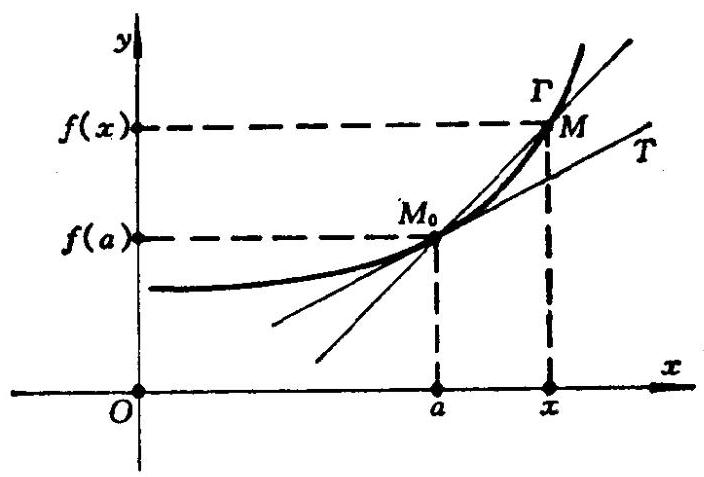
\includegraphics[max width=0.6\textwidth]{images/bo_d25ksc77aajc738obdgg_270_365_745_704_477_0.jpg}
\end{center}
\hspace*{3em} 

图 6-1

如果 $f$ 在 $a$ 处右 (左) 可导,则我们称函数 $f$ 的曲线 $\Gamma$ 在 ${M}_{0}(a$ ,

$f\left( a\right) )$ 处有右 (左) 切线 $T\left( {T}^{\prime }\right)$ .

\begin{center}
	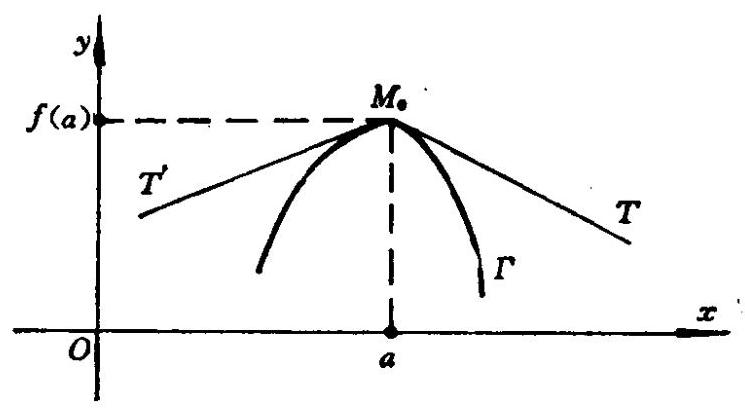
\includegraphics[max width=0.6\textwidth]{images/bo_d25ksc77aajc738obdgg_270_414_1457_745_410_0.jpg}
\end{center}
\hspace*{3em} 

图 6-2

若 $f$ 在 $a$ 处可导,并且 ${f}^{\prime }\left( a\right)  = 0$ ,则曲线 $\Gamma$ 在 ${M}_{0}$ 处的切线 $T$ 平行于 $x$ 轴.

\begin{center}
	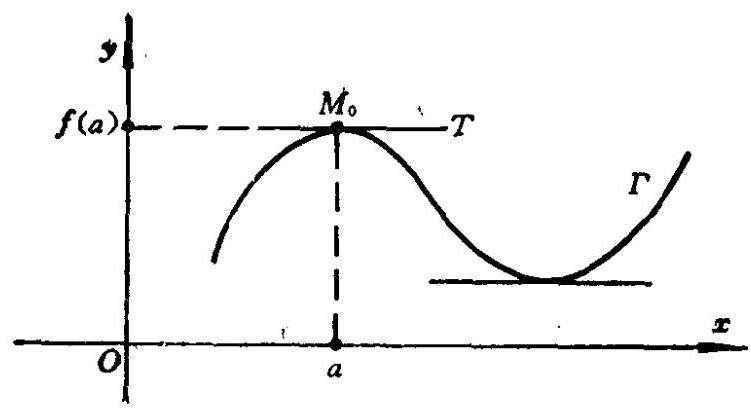
\includegraphics[max width=0.6\textwidth]{images/bo_d25ksc77aajc738obdgg_271_498_264_751_409_0.jpg}
\end{center}
\hspace*{3em} 

图 6-3

关于函数的导数与单侧导数之间的联系, 我们有下述定理.

定理 $6 \cdot  1 \cdot  1$ 设 $f : X \rightarrow  \mathbf{R}$ 是任一函数, $a \in  X$ 是 $X$ 的一个双侧聚点. $f$ 在 $a$ 处可导的充分必要条件是: $f$ 在 $a$ 处左、右可导,并且 ${f}^{\prime }\left( {a}^{ - }\right)  = {f}^{\prime }\left( {a}^{ + }\right)$ . 这时
$${f}^{\prime }\left( {a}^{ - }\right)  = {f}^{\prime }\left( {a}^{ + }\right)  = {f}^{\prime }\left( a\right) .$$

证明 直接由定理 $4 \cdot  1 \cdot  1$ 推出.

\section*{3. 可导性的另一表示法}

定理 $6 \cdot  1 \cdot  2$ 设 $f : X \rightarrow  \mathbf{R}$ 是任一函数, $a \in  X$ 是 $X$ 的一聚点. $f$ 在 $a$ 处可导的充分必要条件是: 存在一个函数 $\varphi  : X \rightarrow  R$ 使得

1) $f\left( x\right)  - f\left( a\right)  = \varphi \left( x\right) \left( {x - a}\right) ,\forall x \in  X$ ,

2) $\varphi$ 在 $a$ 处连续,

这时 ${f}^{\prime }\left( a\right)  = \varphi \left( a\right)$ .

证明 必要性 设 $f$ 在 $a$ 处可导,于是由定义,我们有
$${f}^{\prime }\left( a\right)  = \mathop{\lim }\limits_{{x \rightarrow  a}}\frac{f\left( x\right)  - f\left( a\right) }{x - a}.$$

令
$$\varepsilon \left( x\right)  = \frac{f\left( x\right)  - f\left( a\right) }{x - a} - {f}^{\prime }\left( a\right) ,\;\forall x \in  X - \{ a\} ,$$

则 $\mathop{\lim }\limits_{{x \rightarrow  a}}\varepsilon \left( x\right)  = 0$ . 我们定义函数 $\varphi  : X \rightarrow  \mathbf{R}$ 如下:
$$\varphi \left( x\right)  = {f}^{\prime }\left( a\right)  + \varepsilon \left( x\right) ,\;\forall x \in  X - \{ a\} ,\varphi \left( a\right)  = {f}^{\prime }\left( a\right) .$$

则 $\varphi$ 在 $a$ 处连续,并且
\begin{align*}
	&f\left( x\right)  - f\left( a\right)  = \varphi \left( x\right) \left( {x - a}\right) ,\;\forall x \in  X,\\
	&{f}^{\prime }\left( a\right)  = \varphi \left( a\right) .
\end{align*}

充分性 设存在满足定理条件 1 )与 2 )的函数 $\varphi  : X \rightarrow  \mathbf{R}$ . 那末
$$\frac{f\left( x\right)  - f\left( a\right) }{x - a} = \varphi \left( x\right) ,\;\forall x \in  X - \{ a\} .$$

由 $\varphi$ 在 $a$ 处的连续性推得
$$\mathop{\lim }\limits_{{x \rightarrow  a}}\frac{f\left( x\right)  - f\left( a\right) }{x - a} = \mathop{\lim }\limits_{{x \rightarrow  a}}\varphi \left( x\right)  = \varphi \left( a\right) .$$

此即表明 $f$ 在 $a$ 处可导,并且 ${f}^{\prime }\left( a\right)  = \varphi \left( a\right)$ .

推论 若函数 $f : X \rightarrow  \mathbf{R}$ 在 $a$ 处可导,则 $f$ 在 $a$ 处连续.

证明 因为 $f$ 在 $a$ 处可导,故存在函数 $\varphi  : X \rightarrow  \mathbf{R}$ 使得

$f\left( x\right)  - f\left( a\right)  = \varphi \left( x\right) \left( {x - a}\right) ,\;\forall x \in  X,\varphi$ 在 $a$ 处连续.

令 $x \rightarrow  a$ 立即得到
$$\mathop{\lim }\limits_{{x \rightarrow  a}}f\left( x\right)  = f\left( a\right)$$

因此 $f$ 在 $a$ 处连续.

附注 我们可以把定理 $6 \cdot  1 \cdot  2$ 当作函数 $f$ 在 $a$ 处可导的定义, Caratheodory 在他的著作 (Theory of Functions of a Complex Variable, vol.1 Chelsera, New York, 1954)中就是这样定义函数可导及导数的. 我们可以称他的定义为 Cara-theodory导数定义以区别于Cauchy导数定义.

由于 $\frac{f\left( x\right)  - f\left( a\right) }{x - a} = \varphi \left( x\right)$ 正是联结函数 $f$ 的曲线 $\Gamma$ 上两点 $(a$ , $f\left( a\right) )$ 与 $\left( {x,f\left( x\right) }\right)$ 的割线的斜率,故 Carathéodory 导数定义强调了此割线以连续方式接近 $\Gamma$ 在 $\left( {a,f\left( a\right) }\right)$ 处的切线.

另一方面, Caratheodory 导数定义正像上述推论所指出的, 深刻揭示了在一点可导的函数的重要内在性质——函数在可导点处连续.

以后我们将看到,利用定理 $6 \cdot  1 \cdot  2$ 或 Carathéodory 导数定义证明微分学的许多重要定理要比按Cauchy导数定义去证明更方便, 论述更简洁.

下面我们看几个可导函数的例子.

例1 证明: $\forall n \in  \mathbf{N}$ ,幂函数 $x \mapsto  f\left( x\right)  = {x}^{n},x \in  \mathbf{R}$ 在任一点 $a \in  \mathbf{R}$ 处可导,并且
$${f}^{\prime }\left( a\right)  = n{a}^{n - 1}.$$

事实上,由于 $\forall x \in  R$ ,
$${x}^{n} - {a}^{n} = \left( {x - a}\right) \left( {{x}^{n - 1} + {x}^{n - 2}a + \cdots  + x{a}^{n - 2} + {a}^{n - 1}}\right) .$$

所以对 $x \neq  a$ ,
$$\frac{{x}^{n} - {a}^{n}}{x - a} = {x}^{n - 1} + {x}^{n - 2}a + \cdots  + x{a}^{n - 2} + {a}^{n - 1}.$$

从而
\begin{align*}
	&\mathop{\lim }\limits_{{x \rightarrow  a}}\frac{{x}^{n} - {a}^{n}}{x - a} = \mathop{\lim }\limits_{{x \rightarrow  a}}\left( {{x}^{n - 1} + {x}^{n - 2}a + \cdots  + x{a}^{n - 2} + {a}^{n - 1}}\right)\\
	&= n{a}^{n - 1}\text{ . }
\end{align*}

因此 $f$ 在 $a$ 处可导,并且
$${f}^{\prime }\left( a\right)  = n{a}^{n - 1}.$$

例 2 设函数 $f : \mathbf{R} \rightarrow  \mathbf{R}$ 定义如下:
$$f\left( x\right)  = \left\{  {\begin{array}{ll} {x}^{p}\sin \frac{1}{x}, & x \neq  0, \\  0, & x = 0 \end{array}\left( {p > 1}\right) .}\right.$$

证明: $f$ 在 $x = 0$ 处可导,并且 ${f}^{\prime }\left( 0\right)  = 0$ .

事实上, $\forall x \neq  0$ ,
$$\mathop{\lim }\limits_{{x \rightarrow  0}}\frac{f\left( x\right)  - f\left( 0\right) }{x} = \mathop{\lim }\limits_{{x \rightarrow  0}}{x}^{p - 1}\sin \frac{1}{x} = 0.$$

因此 $f$ 在 $x = 0$ 处可导,并且
$${f}^{\prime }\left( 0\right)  = 0\text{ . }$$

例3 证明: 函数 $x \mapsto  f\left( x\right)  = \left| x\right| ,x \in  \mathbf{R}$ 在 $x = 0$ 处左、右可导,但在 $x = 0$ 处不可导.

事实上, 这时我们有
\begin{align*}
	&\mathop{\lim }\limits_{{x \rightarrow  {0}^{ - }}}\frac{f\left( x\right)  - f\left( 0\right) }{x - 0} = \mathop{\lim }\limits_{{x \rightarrow  {0}^{ - }}}\frac{-x}{x} =  - 1,\\
	&\mathop{\lim }\limits_{{x \rightarrow  {0}^{ + }}}\frac{f\left( x\right)  - f\left( 0\right) }{x - 0} = \mathop{\lim }\limits_{{x \rightarrow  {0}^{ + }}}\frac{x}{x} = 1.
\end{align*}

故 $f$ 在 $x = 0$ 处左、右可导,并且 ${f}^{\prime }\left( {0}^{ - }\right)  =  - 1,{f}^{\prime }\left( {0}^{ + }\right)  = 1$ .

由于 ${f}^{\prime }\left( {0}^{ + }\right)  \neq  {f}^{\prime }\left( {0}^{ - }\right)$ ,故 $f$ 在 $x = 0$ 处不可导.

\section*{4. 无穷大导数}

定义 设 $f : X \rightarrow  \mathbf{R}$ 是任一函数, $a \in  X$ 是 $X$ 的一聚点,我们称 $f$ 在 $a$ 处有正 (负) 无穷大导数,记为 ${f}^{\prime }\left( a\right)  =  + \infty \left( {-\infty }\right)$ ,如果
$$\mathop{\lim }\limits_{{x \rightarrow  a}}\frac{f\left( x\right)  - f\left( a\right) }{x - a} =  + \infty \left( {-\infty }\right) .$$

类似地,我们可以定义下述四种类型的正负无穷大导数:
\begin{align*}
	&{f}^{\prime }\left( {a}^{ + }\right)  =  + \infty ,{f}^{\prime }\left( {a}^{ + }\right)  =  - \infty ,{f}^{\prime }\left( {a}^{ - }\right)  =  + \infty ,\\
	&{f}^{\prime }\left( {a}^{ - }\right)  =  - \infty .
\end{align*}

例 4 证明: 对符号函数 $x \mapsto  \operatorname{sgn}\left( x\right) ,x \in  \mathbf{R}$ 有
$${\operatorname{sgn}}^{\prime }\left( {0}^{ + }\right)  =  + \infty ,{\operatorname{sgn}}^{\prime }\left( {0}^{ - }\right)  =  + \infty .$$

事实上,
\begin{align*}
	&\mathop{\lim }\limits_{{x \rightarrow  {0}^{ + }}}\frac{\operatorname{sgn}\left( x\right)  - \operatorname{sgn}\left( 0\right) }{x - 0} = \mathop{\lim }\limits_{{x \rightarrow  {0}^{ + }}}\frac{1 - 0}{x} =  + \infty ,\\
	&\mathop{\lim }\limits_{{x \rightarrow  {0}^{ - }}}\frac{\operatorname{sgn}\left( x\right)  - \operatorname{sgn}\left( 0\right) }{x - 0} = \mathop{\lim }\limits_{{x \rightarrow  {0}^{ - }}}\frac{-1 - 0}{x} =  + \infty .
\end{align*}

例 5 证明: 对函数 $x \mapsto  f\left( x\right)  = {x}^{\frac{2}{3}},x \in  \mathbf{R}$ 有
$${f}^{\prime }\left( {0}^{ + }\right)  =  + \infty ,{f}^{\prime }\left( {0}^{ - }\right)  =  - \infty .$$

事实上
\begin{align*}
	&\mathop{\lim }\limits_{{x \rightarrow  {0}^{ + }}}\frac{f\left( x\right)  - f\left( 0\right) }{x - 0} = \mathop{\lim }\limits_{{x \rightarrow  {0}^{ + }}}\frac{{x}^{\frac{2}{3}}}{x} = \mathop{\lim }\limits_{{x \rightarrow  {0}^{ + }}}\frac{1}{{x}^{\frac{1}{3}}} =  + \infty ,\\
	&\mathop{\lim }\limits_{{x \rightarrow  {0}^{ - }}}\frac{f\left( x\right)  - f\left( 0\right) }{x - 0} = \mathop{\lim }\limits_{{x \rightarrow  {0}^{ - }}}\frac{{x}^{-\frac{2}{3}}}{x} = \mathop{\lim }\limits_{{x \rightarrow  {0}^{ - }}}\frac{1}{{x}^{\frac{1}{3}}} =  - \infty .
\end{align*}

因此 ${f}^{\prime }\left( {0}^{ + }\right)  =  + \infty ,{f}^{\prime }\left( {0}^{ - }\right)  =  - \infty$ .

\begin{center}
	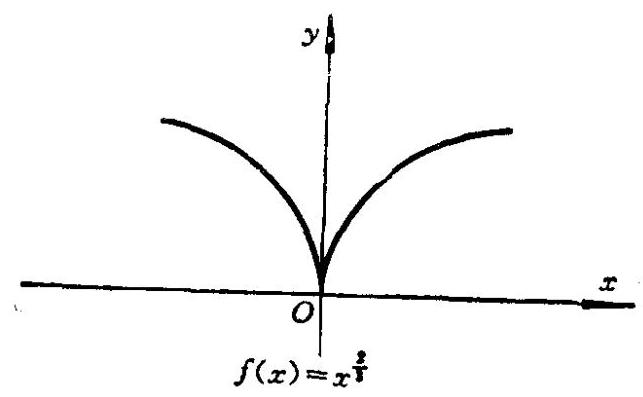
\includegraphics[max width=0.5\textwidth]{images/bo_d25ksc77aajc738obdgg_275_477_292_643_397_0.jpg}
\end{center}
\hspace*{3em} 

图 6-4

\section*{5. 导函数与高阶导数}

定义 设 $f : X \rightarrow  \mathbf{R}$ 是任一函数, $Y \subset  X$ 且 $Y \neq  \varnothing$ .

1)若 $f$ 在 $Y$ 的每一点 $x$ 处可导,则我们称 $f$ 在 $Y$ 上可导. 函数 ${f}^{\prime } : Y \rightarrow  \mathbf{R}$ ,它定义为
$$\left( {f}^{\prime }\right) \left( x\right)  = {f}^{\prime }\left( x\right) ,\;\forall x \in  Y,$$

称为 $f$ 在 $Y$ 上的导函数.

2)若 $f$ 在 $Y$ 上可导,并且导函数 ${f}^{\prime }$ 在 $Y$ 上连续,则 我们称 $f$ 在 $Y$ 上连续可导,或称 $f$ 在 $Y$ 上是 ${C}^{1}$ 类的.

例 6 设 $I \subset  \mathbf{R}$ 是任一区间. $f : I \rightarrow  \mathbf{R}$ 是任一连续函数. $a \in  I$ 是一固定点. 证明: $f$ 的积分函数 $x \mapsto  F\left( x\right)  = {\int }_{a}^{x}f\left( t\right) {dt},x \in  I$ 在 $I$ 上是 ${C}^{1}$ 类的,并且
$${F}^{\prime }\left( x\right)  = f\left( x\right) ,\forall x \in  I.$$

事实上,任取 ${x}_{0} \in  I$ . 由第一积分中值公式
$$F\left( x\right)  - F\left( {x}_{0}\right)  = {\int }_{{x}_{0}}^{x}f\left( t\right) {dt} = f\left( {\xi }_{x}\right) \left( {x - {x}_{0}}\right) ,\forall x \in  I,$$

这里 ${\xi }_{x}$ 介于 ${x}_{0}$ 与 $x$ 之间. 于是 ${\xi }_{x} \rightarrow  {x}_{0}\left( {x \rightarrow  {x}_{0}}\right)$ .

令 $\varphi \left( x\right)  = f\left( {\xi }_{x}\right) ,x \in  I$ ,则函数 $\varphi  : I \rightarrow  \mathbf{R}$ 在 ${x}_{0}$ 处连续, $\varphi \left( {x}_{0}\right)$  $= f\left( {\xi }_{{x}_{0}}\right)  = f\left( {x}_{0}\right)$ . 并且
$$F\left( x\right)  - F\left( {x}_{0}\right)  = \varphi \left( x\right) \left( {x - {x}_{0}}\right) ,\;\forall x \in  I.$$

因此 $F$ 在 ${x}_{0}$ 处可导,并且 ${F}^{\prime }\left( {x}_{0}\right)  = f\left( {x}_{0}\right)$ .

由 ${x}_{0}$ 的任意性知 $F$ 在 $I$ 上可导,并且 $F$ 的导函数 ${F}^{\prime } = f$ . 由于 $f$ 在 $I$ 上连续,故 $F$ 在 $I$ 上是 ${C}^{1}$ 类的.

例7 考虑自然对数函数
$$x \mapsto  \log x = {\int }_{1}^{x}\frac{1}{t}{dt},x \in  {\mathbf{R}}_{ * }^{ + }.$$

由于函数 $x \mapsto  \frac{1}{x},x \in  {\mathbf{R}}_{ * }^{ + }$ 在 ${\mathbf{R}}_{ * }^{ + }$ 上连续,故由例 6 知,自然对数函数 $\log$ 在 ${\mathbf{R}}_{ * }^{ + }$ 上是 ${C}^{1}$ 类的,并且
$${\log }^{\prime }\left( x\right)  = \frac{1}{x},\forall x \in  {\mathbf{R}}_{ * }^{ + }.$$

定义 设 $f : X \rightarrow  \mathbf{R}$ 是任一函数, $a \in  X$ .

1) 若存在 $\delta  > 0$ ,使得 $f$ 在 $Y = X \cap  B\left( {a,\delta }\right)$ 上可导,并且 $f$ 在 $Y$ 上的导函数 ${f}^{\prime } : Y \rightarrow  \mathbf{R}$ 在 $a$ 处可导,则我们称函数 $f$ 在 $a$ 处二次可导, ${f}^{\prime }$ 在 $a$ 处的导数称为 $f$ 在 $a$ 处的二阶导数,记为
$${f}^{\prime \prime }\left( a\right) \text{ 或 }\frac{{d}^{2}f\left( a\right) }{d{x}^{2}}.$$

现在假设 $f$ 在 $Y$ 上的每一点 $x$ 处的 $n - 1$ 阶导数 ${f}^{\left( n - 1\right) }\left( x\right)$ 或 $\frac{{d}^{n - 1}f\left( x\right) }{d{x}^{n - 1}}$ 已经定义,如果函数 $x \mapsto  {f}^{\left( n - 1\right) }\left( x\right) ,x \in  Y$ (称为 $f$ 在 $Y$ 上的 $n - 1$ 阶导函数,记为 ${f}^{\left( n - 1\right) }$ ) 在 $a$ 处可导,则我们称 $f$ 在 $a$ 处 $n$ 次可导, ${f}^{\left( n - 1\right) }$ 在 $a$ 处的导数称为 $f$ 在 $a$ 处的 $n$ 阶导数,记为
$${f}^{\left( n\right) }\left( a\right) \text{ 或 }\frac{{d}^{n}f\left( a\right) }{d{x}^{n}}.$$

子是
$${f}^{\left( n\right) }\left( a\right)  = {\left( {f}^{\left( n - 1\right) }\right) }^{\prime }\left( a\right) .$$

2) 若 $f$ 在 $X$ 的每一点 $x$ 处 $n$ 次可导,则我们称 $f$ 在 $X$ 上 $n$ 次可导.

3) 若 $f$ 在 $X$ 上 $n$ 次可导,并且 $f$ 的 $n$ 阶导函数 ${f}^{\left( n\right) }$ 在 $X$ 上连续, 则我们称 $f$ 在 $X$ 上是 $n$ 次连续可导的,或称 $f$ 在 $X$ 上是 ${C}^{n}$ 类的.

4) 若 $\forall n \in  \mathbf{N}$ ,函数 $f$ 在 $X$ 上是 ${C}^{n}$ 类的,则我们称 $f$ 在 $X$ 上. 是 ${\mathrm{C}}^{\infty }$ 类的.

例 8 证明: 对例 1 的幂函数 $x \mapsto  f\left( x\right)  = {x}^{n},x \in  \mathbf{R}\left( {n \in  \mathbf{N}}\right)$ 有:

1) $\forall k \leq  n,{f}^{\left( k\right) }\left( x\right)  = n\left( {n - 1}\right) \cdots \left( {n - k + 1}\right) {x}^{n - k}\;(\forall x \in$  $\mathbf{R}$ ),

2) $\forall k > n,{f}^{\left( k\right) }\left( x\right)  = 0\;\left( {\forall x \in  \mathbf{R}}\right)$ .

因此 $f$ 在 $\mathbf{R}$ 上是 ${C}^{\infty }$ 类的.

事实上,当 $k = 1$ 时 ${f}^{\prime }\left( x\right)  = n{x}^{n - 1}$ ,结论 1 )成立.

假设当 $k < n$ 时结论 1 )正确,那末当 $k + 1 \leq  n$ 时,我们有
\begin{align*}
	&\frac{{f}^{\left( k\right) }\left( y\right)  - {f}^{\left( k\right) }\left( x\right) }{y - x} = \frac{n\left( {n - 1}\right) \cdots \left( {n - k + 1}\right) \left( {{y}^{n - k} - {x}^{n - k}}\right) }{y - x}\\
	&= n\left( {n - 1}\right) \cdots \left( {n - k + 1}\right) \left( {{y}^{n - k - 1} + {y}^{n - k - 2}x}\right.\\
	&\left. {+\cdots  + {x}^{n - k - 1}}\right) \text{ , }\\
	&\mathop{\lim }\limits_{{y \rightarrow  x}}\frac{{f}^{\left( k\right) }\left( y\right)  - {f}^{\left( k\right) }\left( x\right) }{y - x} = n\left( {n - 1}\right) \cdots \left( {n - k + 1}\right) \mathop{\lim }\limits_{{y \rightarrow  x}}\left( {y}^{n - k - 1}\right.\\
	&\left. {+{y}^{n - k - 2}x + \cdots  + {x}^{n - k - 1}}\right)\\
	&= n\left( {n - 1}\right) \cdots \left( {n - k + 1}\right) \left( {n - k}\right) {x}^{n - k - 1}.
\end{align*}

此即表明 ${f}^{\left( k + 1\right) }\left( x\right)$ 存在,并且 ${f}^{\left( k + 1\right) }\left( x\right)  = n\left( {n - 1}\right) \cdots \left( {n - k}\right) {x}^{n - k - 1}$ 因此结论 1) 成立. 结论 2) 显然. 因为 ${f}^{\left( n\right) }\left( x\right)  = n!$ ,从而 $\forall k$  $> n,{f}^{\left( k\right) }\left( x\right)  \equiv  0$ . 于是 $f$ 在 $\mathbf{R}$ 上是 ${C}^{\infty }$ 类的.

作为这一节的结束, 我们介绍一下一元复值函数的导数.

\section*{6. 一元复值函数的导数}

设 $X \subset  \mathbf{R},f : X \rightarrow  \mathbf{C}$ 是任一复值函数. 令
$$f\left( x\right)  = {f}_{1}\left( x\right)  + i{f}_{2}\left( x\right) ,\forall x \in  X.$$

于是 ${f}_{1},{f}_{2} : X \rightarrow  \mathbf{R}$ 是两个一元实值函数.

定义: $f,{f}_{1},{f}_{2}$ 如上所述

1) 我们称 $f$ 在 $x \in  X$ 处可导,如果 ${f}_{1},{f}_{2}$ 在 $x$ 处可导,并立这时 $f$ 在 $x$ 处的导数 ${f}^{\prime }\left( x\right)$ ,定义为
$${f}^{\prime }\left( x\right)  = {f}_{1}^{\prime }\left( x\right)  + i{f}_{2}^{\prime }\left( x\right) .$$

2) 我们称 $f$ 在 $X$ 上可导,如果 $f$ 在 $X$ 上的每一点处可导.

3) 我们称 $f$ 在 $X$ 上是 ${C}^{n}$ 类的 $\left( {n \geq  1}\right)$ ,如果 ${f}_{1},{f}_{2}$ 在 $X$ 上是 ${C}^{n}$ 类的.

4) 我们称 $f$ 在 $X$ 上是 ${C}^{\infty }$ 类的,如果 $\forall n \in  \mathbf{N},f$ 在 $X$ 上 是 ${C}^{\infty }$ 类的.

由上述定义可知,若 $f$ 在 $X$ 上是 ${C}^{n}$ 类的,则
$${f}^{\left( n\right) }\left( x\right)  = {f}_{1}^{\left( n\right) }\left( x\right)  + i{f}_{2}^{\left( n\right) }\left( x\right) ,\;\forall x \in  X.$$

\section*{习 题}

1. 考虑Dirichlet函数 $x \mapsto  D\left( x\right)  = \left\{  \begin{array}{ll} 1, & x \in  \mathbf{Q}, \\  0, & x \in  {\mathbf{Q}}^{\bar{c}}. \end{array}\right.$ .

1) 证明: $D$ 在 $\mathrm{R}$ 的任一点 $x$ 处都不可导.

2) 证明: 函数 $x \mapsto  g\left( x\right)  = {x}^{2}D\left( x\right) ,x \in  R$ 只在 $x = 0$ 处可导,并且 ${g}^{\prime }\left( 0\right)  = 0$ .

2. 设 $a \in  R$ ,并且 $a > 0$ . 证明: 函数 $x \mapsto  {\left| x\right| }^{a},x \in  R$ 在 $x = 0$ 处可导的充分必要条件是 $a > 1$ .

3. 设函数 $f,g,h : X \rightarrow  \mathbf{R}$ 在点 $a \in  X$ 处满足下述条件:

1) $f\left( a\right)  = g\left( a\right)  = h\left( a\right) ,{f}^{\prime }\left( a\right)  = {g}^{\prime }\left( a\right)$ ;

2) $f\left( x\right)  \leq  h\left( x\right)  \leq  g\left( x\right) ,\forall x \in  X$ .

证明: $h$ 在 $a$ 处可导,并且 ${h}^{\prime }\left( a\right)  = {f}^{\prime }\left( a\right)  = {g}^{\prime }\left( a\right)$ .

4. 设 $a,b \in  R$ ,考虑函数
$$x \mapsto  f\left( x\right)  = \left\{  {\begin{array}{ll} {x}^{2}, & x \geq  {x}_{0}, \\  {ax} + b, & x < {x}_{0}, \end{array}.}\right.$$

试选择常数 $a$ 与 $b$ 使得 $f$ 在 ${x}_{0}$ 处可导.

5. 证明:函数
$$x \mapsto  f\left( x\right)  = \left\{  \begin{array}{ll} {x}^{2}\left| {\sin \frac{\pi }{x}}\right| , & x \neq  0; \\  0, & x = 0. \end{array}\right.$$

在 $x = 0$ 的任何邻域内都有不可导的点. 但在 $x = 0$ 处可导,并且 ${f}^{\prime }\left( 0\right)  = 0$ .

6. 设 $I \subset  R$ 是一开区间, $0 \in  I,f : I \rightarrow  R$ 在 $x = 0$ 处连续,并且 $f\left( 0\right)  = 0$ . 证明: 若 $\mathop{\lim }\limits_{{x \rightarrow  0}}\frac{f\left( {2x}\right)  - f\left( x\right) }{x} = A \in  \mathbf{R}$ ,则 $f$ 在 $x = 0$ 处可导,并且 ${f}^{\prime }\left( 0\right)  = A$ .

7. 设 $f : I \rightarrow  R$ 是任一函数, $a \in  I$ 是一内点使得 $B\left( {a,\delta }\right)  \subset  I$ . 令 $H =$  $\{ h \in  R \mid  \left| h\right|  < \delta \}$ . 如果存在函数 $\varphi  : H \rightarrow  R$ 使得

1) $f\left( {a + h}\right)  - f\left( {a - h}\right)  = \varphi \left( h\right) {2h}\;\forall h \in  H$ ,

2) $\varphi$ 在 $h = 0$ 处连续.

则称 $\varphi \left( 0\right)$ 为函数 $f$ 在 $a$ 处的对称导数,记为 ${f}^{\prime }{}_{s}\left( a\right)  = \varphi \left( 0\right)$ .

1) 证明: 若 $f$ 在 $a$ 处的左、右导数存在,则 $f$ 在 $a$ 处的对称导数存在.

2) 证明: 函数
$$x \mapsto  f\left( x\right)  = \left\{  \begin{array}{ll} x\sin \frac{1}{x}, & x \neq  0; \\  0, & x = 0 \end{array}\right.$$

在 $x = 0$ 处有对称导数存在,但在 $x = 0$ 处的左、右导数都不存在.

8. 设函数 $f : \left\lbrack  {a,b}\right\rbrack   \rightarrow  R$ 在 $\left\lbrack  {a,b\left\lbrack  \right. }\right.$ 的每一点 $x$ 处有右导数 ${f}^{\prime }\left( {x}^{ + }\right)$ 存在. 证明: 存在一个开区间 $\rbrack \alpha ,\beta \left\lbrack   \subset  \right\rbrack  a,b\left\lbrack  {\text{ ，使得 }f\text{ 在 }}\right\rbrack  \alpha ,\beta \lbrack$ 上连续.

9. 证明: 函数 $f : R \rightarrow  R$
$$f\left( x\right)  = \left\{  \begin{array}{ll} {x}^{2n}\sin \frac{1}{x}, & x \neq  0; \\  0, & x = 0. \end{array}\right.$$

在 $x = 0$ 处 ${f}^{\prime }\left( 0\right) ,{f}^{\prime \prime }\left( 0\right) ,\cdots ,{f}^{\left( n\right) }\left( 0\right)$ 存在,但 ${f}^{\left( n + 1\right) }\left( 0\right)$ 不存在。

10. 设函数 $f : R \rightarrow  R$ 定义如下:
$$f\left( x\right)  = \left\{  \begin{array}{l} {x}^{n} \cdot  x > 0, \\  0,x \leq  0. \end{array}\right.$$

证明: $f$ 在 $\mathrm{R}$ 上 $n - 1$ 次可导,但 $f$ 在 $x = 0$ 处不是 $n$ 次可导的.

11. 设 $f : \left\lbrack  {a,b}\right\rbrack   \rightarrow  \mathbf{R}$ 是任一 ${C}^{1}$ 类函数, $f\left( a\right)  = 0$ . 试利用定积分的 Cauchy 积分不等式证明
$${\int }_{a}^{b}{f}^{2}\left( x\right) {dx} \leq  \frac{{\left( b - a\right) }^{2}}{2}{\int }_{a}^{b}{\left\lbrack  {f}^{\prime }\left( x\right) \right\rbrack  }^{2}{dx}.$$

12. 设函数 $f : \left\lbrack  {a,b}\right\rbrack   \rightarrow  R$ 可导,导函数 ${f}^{\prime } : \left\lbrack  {a,b}\right\rbrack   \rightarrow  R$ 在 $\left\lbrack  {a,b}\right\rbrack$ 上可积,

令
$${S}_{n} = \frac{b - a}{n}\mathop{\sum }\limits_{{k = 1}}^{n}f\left( {a + \left( {k - 1}\right) \frac{b - a}{n}}\right) {f}^{\prime }\left( {a + k\frac{b - a}{n}}\right) .$$

试计算极限 $\mathop{\lim }\limits_{{n \rightarrow   + \infty }}{S}_{n}$ .

13. 设 $\alpha ,\beta  \in  R$ ,令
$$E\left( {\alpha ,\beta }\right)  = \left\{  {f \in  {C}^{1}\left( {\left\lbrack  {a,b}\right\rbrack  ,R}\right)  \mid  f\left( a\right)  = \alpha ,f\left( b\right)  = \beta }\right\}  .$$

${f}_{0}$ 是 $E\left( {\alpha ,\beta }\right)$ 中的仿射映射,即 ${f}_{0}\left( x\right)  = {Ax} + B$ . 试对 ${f}_{0}$ 与 $f \in  E\left( {\alpha ,\beta }\right)$ 应用 Cauchy积分不等式证明
$$\forall j \in  E\left( {\alpha ,\beta }\right) ,{\int }_{a}^{b}{\left\lbrack  {f}^{\prime }\left( x\right) \right\rbrack  }^{2}{dx} \geq  {\int }_{a}^{b}{\left\lbrack  {f}^{\prime }{}_{0}\left( x\right) \right\rbrack  }^{2}{dx}.$$

\section{导数的计算}

首先我们介绍导数计算的一般法则.

\section*{1. 导数计算的一般法则}

定理 $6 \cdot  2 \cdot  1$ 设函数 $f,g : X \rightarrow  \mathbf{R}$ 在 $a \in  X$ 处可导. 则

1) $\forall \alpha ,\beta  \in  \mathbf{R}$ ,函数 ${\alpha f} + {\beta g} : X \rightarrow  \mathbf{R}$ 在 $a$ 处可导,并且
$${\left( \alpha f + \beta g\right) }^{\prime }\left( a\right)  = \alpha {f}^{\prime }\left( a\right)  + \beta {g}^{\prime }\left( a\right) .$$

2) 函数 ${fg} : X \rightarrow  \mathbf{R}$ 在 $a$ 处可导,并且
$${\left( fg\right) }^{\prime }\left( a\right)  = {f}^{\prime }\left( a\right) g\left( a\right)  + f\left( a\right) {g}^{\prime }\left( a\right) .$$

3) 当 $g\left( a\right)  \neq  0$ 时,存在 $\delta  > 0$ 使得函数 $\frac{f}{g} : X \cap  B\left( {a,\delta }\right)  \rightarrow  \mathbf{R}$ 在 $a$ 处可导,并且
$${\left( \frac{f}{g}\right) }^{\prime }\left( a\right)  = \frac{{f}^{\prime }\left( a\right) g\left( a\right)  - f\left( a\right) {g}^{\prime }\left( a\right) }{{g}^{2}\left( a\right) }.$$

证明 因为 $f,g$ 在 $a$ 处可导,故根据定理 $6 \cdot  1 \cdot  2$ 知,存在函数 $\varphi ,\psi  : X \rightarrow  \mathbf{R}$ 使得

i) $f\left( x\right)  - f\left( a\right)  = \varphi \left( x\right) \left( {x - a}\right) ,g\left( x\right)  - g\left( a\right)  = \psi \left( x\right) \left( {x - a}\right)$ , $\forall x \in  X,$

ii) $\varphi ,\psi$ 在 $a$ 处连续, $\varphi \left( a\right)  = {f}^{\prime }\left( a\right) ,\psi \left( a\right)  = {g}^{\prime }\left( a\right)$ . 于是 $\forall \alpha ,\beta  \in  \mathbf{R},\forall x \in  \mathbf{R}$ 我们有
\begin{align*}
	&\left( {{\alpha f} + {\beta g}}\right) \left( x\right)  - \left( {{\alpha f} + {\beta g}}\right) \left( a\right)  = \alpha \left\lbrack  {f\left( x\right)  - f\left( a\right) }\right\rbrack\\
	&+ \beta \left\lbrack  {g\left( x\right)  - g\left( a\right) }\right\rbrack   = \left\lbrack  {{\alpha \varphi }\left( x\right)  + {\beta \psi }\left( x\right) }\right\rbrack  \left( {x - a}\right) ,\\
	&\left( {fg}\right) \left( x\right)  - \left( {fg}\right) \left( a\right)  = \left\lbrack  {f\left( x\right)  - f\left( a\right) }\right\rbrack  g\left( x\right)  + f\left( a\right) \lbrack g\left( x\right)\\
	&- g\left( a\right) \rbrack  = \left\lbrack  {\varphi \left( x\right) g\left( x\right)  + f\left( a\right) \psi \left( x\right) }\right\rbrack  \left( {x - a}\right) .
\end{align*}

若我们令: $\forall x \in  X$
$$h\left( x\right)  = {\alpha \varphi }\left( x\right)  + {\beta \psi }\left( x\right) ,k\left( x\right)  = \varphi \left( x\right) g\left( x\right)  + f\left( a\right) \psi \left( x\right) ,$$

则函数 $h,k : X \rightarrow  \mathbf{R}$ 在 $a$ 处连续,并且
\begin{align*}
	&\left( {{\alpha f} + {\beta g}}\right) \left( x\right)  - \left( {{\alpha f} + {\beta g}}\right) \left( a\right)  = h\left( x\right) \left( {x - a}\right) ,\;\forall x \in  X,\\
	&\left( {fg}\right) \left( x\right)  - \left( {fg}\right) \left( a\right)  = k\left( x\right) \left( {x - a}\right) ,\;\forall x \in  X.
\end{align*}

因此根据定理 $6 \cdot  1 \cdot  2$ 知,函数 ${\alpha f} + {\beta g},{fg}$ 在 $a$ 处可导,并且
\begin{align*}
	&{\left( \alpha f + \beta g\right) }^{\prime }\left( a\right)  = h\left( a\right)  = {\alpha \varphi }\left( a\right)  + {\beta \psi }\left( a\right)  = \alpha {f}^{\prime }\left( a\right)  + \beta {g}^{\prime }\left( a\right) ,\\
	&{\left( fg\right) }^{\prime }\left( a\right)  = k\left( a\right)  = \varphi \left( a\right) g\left( a\right)  + f\left( a\right) \psi \left( a\right)  = {f}^{\prime }\left( a\right) g\left( a\right)\\
	&+ f\left( a\right) {g}^{\prime }\left( a\right) \text{ . }
\end{align*}

最后由于 $g\left( a\right)  \neq  0$ ,故由 $g$ 在 $a$ 处的连续性知,存在 $\delta  > 0$ ,使得 $g\left( x\right)  \neq  0,\forall x \in  X \cap  B\left( {a,\delta }\right)$ . 于是
\begin{align*}
	&\frac{f}{g}\left( x\right)  - \frac{f}{g}\left( a\right)  = \frac{f\left( x\right) g\left( a\right)  - f\left( a\right) g\left( x\right) }{g\left( a\right) g\left( x\right) }\\
	&= \frac{\left\lbrack  {f\left( x\right)  - f\left( a\right) }\right\rbrack  g\left( a\right)  - f\left( a\right) \left\lbrack  {g\left( x\right)  - g\left( a\right) }\right\rbrack  }{g\left( a\right) g\left( x\right) }\\
	&= \frac{\left\lbrack  \varphi \left( x\right) g\left( a\right)  - f\left( a\right) \psi \left( x\right) \right\rbrack  }{g\left( a\right) g\left( x\right) }\left( {x - a}\right) ,\\
	&\forall x \in  X \cap  B\left( {a,\delta }\right) .
\end{align*}

令 $s\left( x\right)  = \frac{\varphi \left( x\right) g\left( a\right)  - f\left( a\right) \psi \left( x\right) }{g\left( a\right) g\left( x\right) },\forall x \in  X \cap  B\left( {a,\delta }\right)$ ,则函

数 $s : X \cap  B\left( {a,\delta }\right)  \rightarrow  \mathbf{R}$ 在 $a$ 处连续,并且
$$\frac{f}{g}\left( x\right)  - \frac{f}{g}\left( a\right)  = s\left( x\right) \left( {x - a}\right) ,\;\forall x \in  X \cap  B\left( {a,\delta }\right) .$$

因此函数 $\frac{f}{g} : X \cap  B\left( {a,\delta }\right)  \rightarrow  \mathbf{R}$ 在 $a$ 处可导,并且
\begin{align*}
	&{\left( \frac{f}{g}\right) }^{\prime }\left( a\right)  = s\left( a\right)  = \frac{\varphi \left( a\right) g\left( a\right)  - f\left( a\right) \psi \left( a\right) }{g{\left( a\right) }^{2}}\\
	&= \frac{{f}^{\prime }\left( a\right) g\left( a\right)  - f\left( a\right) {g}^{\prime }\left( a\right) }{{g}^{2}\left( a\right) }.
\end{align*}

例1 证明: 对函 数 $x \mapsto  {x}^{n},x \in  \mathrm{R} - \{ 0\} ,\left( {n \in  \mathrm{Z}-\{ 0\} }\right)$ ,
$${\left( {x}^{n}\right) }^{\prime } = n{x}^{n - 1}$$

事实上,若 $n \in  \mathbf{N}$ ,则在 $§1$ 例 1 中已证
$${\left( {x}^{n}\right) }^{\prime } = n{x}^{n - 1}$$

若 $n \in   - \mathbf{N}$ ,则 $- n \in  \mathbf{N}$ ,由上述定理知
\begin{align*}
	&{\left( {x}^{n}\right) }^{\prime } = {\left( \frac{1}{{x}^{-n}}\right) }^{\prime } = \frac{{1}^{\prime } \cdot  {x}^{-n} - 1 \cdot  {\left( {x}^{-n}\right) }^{\prime }}{{x}^{-{2n}}} = \frac{-\left( {-n}\right) {x}^{-n - 1}}{{x}^{-{2n}}}\\
	&= n{x}^{n - 1}\text{ . }
\end{align*}

定理 $6 \cdot  2 \cdot  2$ (复合函数的导数) 设函数 $f : X \rightarrow  \mathbf{R}$ 与函数 $g : Y$  $\rightarrow  \mathrm{R}$ 满足下述条件:

1) $a$ 是 $Z = X \cap  {f}^{-1}\left( Y\right)$ 的聚点.

2) $f$ 在 $a \in  X$ 处可导, $g$ 在 $b \in  Y$ 处可导,且 $b = f\left( a\right)$ 则复合函数 $g \circ  f : Z \rightarrow  \mathbf{R}$ 在 $a$ 处可导,并且
$${\left( g \circ  f\right) }^{\prime }\left( a\right)  = {g}^{\prime }\left( b\right)  \cdot  {f}^{\prime }\left( a\right) .$$

证明 由于 $f$ 在 $a$ 处可导, $g$ 在 $b$ 处可导,故存在函数 $\varphi  : X \rightarrow  \mathbf{R}$ 及函数 $\psi  : Y \rightarrow  \mathbf{R}$ 使得

i) $f\left( x\right)  - f\left( a\right)  = \varphi \left( x\right) \left( {x - a}\right) \forall x \in  X;\varphi$ 在 $a$ 处连续, $\varphi \left( a\right)$  $= {f}^{\prime }\left( a\right)$ .

ii) $g\left( y\right)  - g\left( b\right)  = \psi \left( y\right) \left( {y - b}\right) ,\forall y \in  Y;\psi$ 在 $b$ 处连续, $\psi \left( b\right)$  $= {g}^{\prime }\left( b\right)$ .

于是 $\forall x \in  Z = X \cap  {f}^{-1}\left( Y\right)$ ,
\begin{align*}
	&g \circ  f\left( x\right)  - g \circ  f\left( a\right)  = g\left( {f\left( x\right) }\right)  - g\left( {f\left( a\right) }\right)\\
	&= \psi \left( {f\left( x\right) }\right) \left\lbrack  {f\left( x\right)  - f\left( a\right) }\right\rbrack\\
	&= \psi \left( {f\left( x\right) }\right) \varphi \left( x\right) \left( {x - a}\right)\\
	&= \left( {\psi  \circ  f}\right)  \cdot  \varphi \left( x\right) \left( {x - a}\right) ,
\end{align*}

由于函数 $\left( {\psi  \circ  f}\right) \varphi  : Z \rightarrow  R$ 在 $a$ 处连续,故由定理 $6 \cdot  1 \cdot  2$ 知 $g \circ  f$ 在 $a$ 处可导, 并且
$${\left( g \circ  f\right) }^{\prime }\left( a\right)  = \left( {\psi  \circ  f}\right)  \cdot  \varphi \left( a\right)  = \psi \left( {f\left( a\right) }\right)  \cdot  \varphi \left( a\right)  = {g}^{\prime }\left( b\right)  \cdot  {f}^{\prime }\left( a\right) .$$

定理 $6 \cdot  2 \cdot  3$ (反函数的导数) 设 $X,Y \subset  \mathbf{R}$ 是两个非空集合. $f : X \rightarrow  Y$ 与 ${f}^{-1} : Y \rightarrow  X$ 互为反函数, $a \in  X,b = f\left( a\right)  \in  Y$ ,此外还假设

1) $f$ 在 $a$ 处可导,并且 ${f}^{\prime }\left( a\right)  \neq  0$ ;

2) ${f}^{-1}$ 在 $b$ 处连续,

则 ${f}^{-1}$ 在 $b$ 处可导,并且
$${\left( {f}^{-1}\right) }^{\prime }\left( b\right)  = \frac{1}{{f}^{\prime }\left( a\right) }.$$

证明 首先由于 $f$ 是可逆的,并且 $a$ 是 $X$ 的聚点,故 $b = f\left( a\right)$ 是 $Y$ 的聚点. 由假设 $f$ 在 $a$ 处可导知,存在函数 $\varphi  : X \rightarrow  \mathbf{R}$ 使得

i) $f\left( x\right)  - f\left( a\right)  = \varphi \left( x\right) \left( {x - a}\right) ,\forall x \in  X$ ;

ii) $\varphi$ 在 $a$ 处连续,并且 $\varphi \left( a\right)  = {f}^{\prime }\left( a\right)$ .

由于 $\varphi \left( a\right)  \neq  0$ ,不失一般性,我们可以假设 $\forall x \in  X,\varphi \left( x\right)  \neq  0$ .

现在令 $x = {f}^{-1}\left( y\right) \left( {\forall y \in  Y}\right)$ ,则 $\varphi \left( {{f}^{-1}\left( y\right) }\right)  \neq  0,\forall y \in  Y$ . 并且.
$$f\left( {{f}^{-1}\left( y\right) }\right)  - f\left( {{f}^{-1}\left( b\right) }\right)  = \varphi \left( {{f}^{-1}\left( y\right) }\right) \left\lbrack  {{f}^{-1}\left( y\right)  - {f}^{-1}\left( b\right) }\right\rbrack$$

或
$${f}^{-1}\left( y\right)  - {f}^{-1}\left( b\right)  = \frac{1}{\varphi \left( {{f}^{-1}\left( y\right) }\right) }\left( {y - b}\right) ,\;\forall y \in  Y.$$

由于 ${f}^{-1}$ 在 $b$ 处连续,故函数 $\varphi  \circ  {f}^{-1} : Y \rightarrow  \mathbf{R}$ 在 $b$ 处连续,根据定理 $6 \cdot  1 \cdot  2$ 知, ${f}^{-1}$ 在 $b$ 处可导,并且
$${\left( {f}^{-1}\right) }^{\prime }\left( b\right)  = \frac{1}{\varphi \left( {{f}^{-1}\left( b\right) }\right) } = \frac{1}{\varphi \left( a\right) } = \frac{1}{{f}^{\prime }\left( a\right) }.$$

附注 如果我们预先知道 $f$ 的反函数 ${f}^{-1}$ 在 $b = f\left( a\right)$ 处可导, 那末由恒等式
$${f}^{-1} \circ  f\left( x\right)  = i{d}_{X}\left( x\right) ,\;\forall x \in  X,$$

分别对等式两边的函数求在 $a$ 处的导数,根据定理 $6 \cdot  2 \cdot  2$ ,我们得到
$${\left( {f}^{-1}\right) }^{\prime }\left( b\right)  \cdot  {f}^{\prime }\left( a\right)  = 1.$$

若 ${f}^{\prime }\left( a\right)  \neq  0$ ,则 ${\left( {f}^{-1}\right) }^{\prime }\left( b\right)  = \frac{1}{{f}^{\prime }\left( a\right) }$ .

定理 $6 \cdot  2 \cdot  4$ (Leibniz公式) 设函数 $f,g : X \rightarrow  \mathbf{R}$ 在 $a \in  X$ 处 $n$ 次可导,则函数 ${fg} : X \rightarrow  \mathbf{R}$ 在 $a$ 处 $n$ 次可导,并且
\begin{align*}
	&{\left( fg\right) }^{\left( n\right) }\left( a\right)  = {f}^{\left( n\right) }\left( a\right) g\left( a\right)  + {C}_{n}^{1}{f}^{\left( n - 1\right) }\left( a\right) {g}^{\prime }\left( a\right)\\
	&+ {C}_{n}^{2}{f}^{\left( n - 2\right) }\left( a\right) {g}^{\prime \prime }\left( a\right)  + \cdots  + {C}_{n}^{k}{f}^{\left( n - k\right) }\left( a\right) {g}^{\left( k\right) }\left( a\right)\\
	&+ \cdots  + {C}_{n}^{n - 1}{f}^{\prime }\left( a\right) {g}^{\left( n - 1\right) }\left( a\right)  + f\left( a\right) {g}^{\left( n\right) }\left( a\right) .
\end{align*}

证明 我们对 $n$ 用数学归纳法证明.

当 $n = 1$ 时,上述公式化为 ${\left( fg\right) }^{\prime }\left( a\right)  = {f}^{\prime }\left( a\right) g\left( a\right)  + f\left( a\right) {g}^{\prime }\left( a\right)$ 这就是定理 $6 \cdot  2 \cdot  1$ 的 2 ).

现在假设当 $n = m$ 时 Leibniz 公式成立,那末当 $n = m + 1$ 时, 我们有
\begin{align*}
	&{\left( fg\right) }^{\left( m + 1\right) }\left( a\right)  = \left\lbrack  {\left( fg\right) }^{\left( m\right) }\right\rbrack  \prime \left( a\right)\\
	&= {\left( {f}^{\left( m\right) }g\right) }^{\prime }\left( a\right)  + {C}_{m}^{1}{\left( {f}^{\left( m - 1\right) }{g}^{\prime }\right) }^{\prime }\left( a\right)  + {C}_{m}^{2}{\left( {f}^{\left( m - 2\right) }{g}^{\prime \prime }\right) }^{\prime }\left( a\right)\\
	&+ \cdots  + {C}_{m}^{k - 1}{\left( {f}^{\left( m - k + 1\right) }{g}^{\left( k - 1\right) }\right) }^{\prime }\left( a\right)  + {C}_{m}^{k}{\left( {f}^{\left( m - k\right) }{g}^{\left( k\right) }\right) }^{\prime }\left( a\right)\\
	&+ \cdots  + {\left( f{g}^{\left( m\right) }\right) }^{\prime }\left( a\right)\\
	&= {f}^{\left( m + 1\right) }\left( a\right) g\left( a\right)  + {f}^{\left( m\right) }\left( a\right) {g}^{\prime }\left( a\right)\\
	&+ {C}_{m}^{1}{f}^{\left( m\right) }\left( a\right) {g}^{\prime }\left( a\right)  + {C}_{m}^{1}{f}^{\left( m - 1\right) }\left( a\right) {g}^{\prime \prime }\left( a\right)\\
	&+ {C}_{m}^{2}{f}^{\left( m - 1\right) }\left( a\right) {g}^{\prime \prime }\left( a\right)  + {C}_{m}^{2}{f}^{\left( m - 2\right) }\left( a\right) {g}^{\prime \prime \prime }\left( a\right)  + \cdots\\
	&+ {C}_{m}^{k - 1}{f}^{\left( m - k + 2\right) }\left( a\right) {g}^{\left( k - 1\right) }\left( a\right)  + {C}_{m}^{k - 1}{f}^{\left( m - k + 1\right) }\left( a\right) {g}^{\left( k\right) }\left( a\right)
\end{align*}
\begin{align*}
	&+ {C}_{m}^{k}{f}^{\left( m - k + 1\right) }\left( a\right) {g}^{\left( k\right) }\left( a\right)  + {C}_{m}^{k}{f}^{\left( m - k\right) }\left( a\right) {g}^{\left( k + 1\right) }\left( a\right)\\
	&+ \cdots  + {f}^{\prime }\left( a\right) {g}^{\left( m\right) }\left( a\right)  + f\left( a\right) {g}^{\left( m + 1\right) }\left( a\right)\\
	&= {f}^{\left( m + 1\right) }\left( a\right) g\left( a\right)  + \left( {{C}_{m}^{0} + {C}_{m}^{1}}\right) {f}^{\left( m\right) }\left( a\right) {g}^{\prime }\left( a\right)\\
	&+ \left( {{C}_{m}^{1} + {C}_{m}^{2}}\right) {f}^{\left( m - 1\right) }\left( a\right) {g}^{\prime \prime }\left( a\right)\\
	&+ \cdots  + \left( {{C}_{m}^{k - 1} + {C}_{m}^{k}}\right) {f}^{\left( m - k + 1\right) }\left( a\right) {g}^{\left( k\right) }\left( a\right)\\
	&+ \cdots  + f\left( a\right) {g}^{\left( m + 1\right) }\left( a\right)\\
	&= {f}^{\left( n + 1\right) }\left( a\right) g\left( a\right)  + {C}_{n + 1}^{1}{f}^{\left( n\right) }\left( a\right) {g}^{\prime }\left( a\right)\\
	&+ {C}_{m + 1}^{2}{f}^{\left( m - 1\right) }\left( a\right) {g}^{\prime \prime }\left( a\right)  + \cdots  + {C}_{m + 1}^{k}{f}^{\left( m - k + 1\right) }\left( a\right) {g}^{\left( k\right) }\left( a\right)
\end{align*}
$$+ \cdots  + f\left( a\right) {g}^{\left( m + 1\right) }\left( a\right) \text{ . }$$

(这里我们利用了组合公式 ${C}_{m}^{k - 1} + {C}_{m}^{k} = {C}_{m + 1}^{k},\forall k = 1,\cdots ,m$ ). 此即表明 $n = m + 1$ 时, Leibniz公式成立. 由归纳法知, $\forall n \in  \mathbf{N}$ , Leibniz公式成立.

作为导数计算法则的应用, 我们下面来计算基本初等函数的导数.

\section*{2. 基本初等函数的导数}

\section*{1)三角函数的导数}

$x \mapsto  \sin x,x \in  \mathbf{R}$ 的导数 $\forall a \in  \mathbf{R}$ ,由于
$$\sin x - \sin a = 2\sin \frac{x - a}{2}\cos \frac{x + a}{2},\;\forall x \in  \mathbf{R},$$

故
\begin{align*}
	&\mathop{\lim }\limits_{{x \rightarrow  a}}\frac{\sin x - \sin a}{x - a} = \mathop{\lim }\limits_{{x \rightarrow  a}}2\frac{\sin \frac{x - a}{2}}{x - a}\cos \frac{x + a}{2}\\
	&= \mathop{\lim }\limits_{{x \rightarrow  a}}\frac{\sin \frac{x - a}{2}}{\frac{x - a}{2}}\mathop{\lim }\limits_{{x \rightarrow  a}}\cos \frac{x + a}{2}\\
	&= \cos a\text{ . }
\end{align*}

因此正弦函数 $x \mapsto  \sin x,x \in  \mathbf{R}$ 在 $a$ 处可导,并且 ${\sin }^{\prime }\left( a\right)  = \cos a$ . 由 $a$ 的任意性我们得到
$${\sin }^{\prime }x = \cos x,\;\forall x \in  \mathbf{R}.$$

$x \mapsto  \cos x,x \in  \mathbf{R}$ 的导数 由于
$$\cos x = \sin \left( {\frac{\pi }{2} - x}\right) ,\;\forall x \in  \mathbf{R}.$$

故由定理 $6 \cdot  2 \cdot  2$ 知,余弦函数 $x \mapsto  \cos x,x \in  \mathbf{R}$ 在任一点 $x$ 处可导,

并且.
\begin{align*}
	&{\cos }^{\prime }\left( x\right)  = {\sin }^{\prime }\left( {\frac{\pi }{2} - x}\right)  \cdot  {\left( \frac{\pi }{2} - x\right) }^{\prime }\\
	&= \cos \left( {\frac{\pi }{2} - x}\right)  \cdot  \left( {-1}\right)  =  - \sin x.
\end{align*}

因此
$${\cos }^{\prime }x =  - \sin x,\forall x \in  \mathbf{R}.$$

$x \mapsto  \operatorname{tg}x,x \in  \mathbf{R} - \left\{  {{k\pi } + \frac{\pi }{2} \mid  k \in  \mathbf{Z}}\right\}$ 的导数 由于
$$\operatorname{tg}x = \frac{\sin x}{\cos x},\;\forall x \in  \mathbf{R} - \left\{  {{k\pi } + \frac{\pi }{2} \mid  k \in  \mathbf{Z}}\right\}  ,$$

故由定理 $6 \cdot  2 \cdot  1$ 知正切函数
$$x \mapsto  \operatorname{tg}x,x \in  \mathbf{R} - \left\{  {{k\pi } + \frac{\pi }{2} \mid  k \in  \mathbf{Z}}\right\}  \text{ 在任一点 }x \in  \mathbf{R} - \{ {k\pi }$$

$\left. {\left. {+\frac{\pi }{2}}\right| \;k \in  \mathbf{Z}}\right\}$ 处可导,并且
$${\operatorname{tg}}^{\prime }x = \frac{{\sin }^{\prime }x\cos x - {\cos }^{\prime }x\sin x}{{\cos }^{2}x} = \frac{{\cos }^{2}x + {\sin }^{2}x}{{\cos }^{2}x} = \frac{1}{{\cos }^{2}x}.$$

因此
$${\operatorname{tg}}^{\prime }x = \frac{1}{{\cos }^{2}x},\;\forall x \in  \mathbf{R} - \left\{  {{k\pi } + \frac{\pi }{2} \mid  k \in  \mathbf{Z}}\right\}  .$$

$x \mapsto  \operatorname{ctg}x,x \in  \mathbf{R} - \{ {k\pi } \mid  k \in  \mathbf{Z}\}$ 的导数 由于
$$\operatorname{ctg}x = \frac{\cos x}{\sin x},\;\forall x \in  \mathbf{R} - \{ {k\pi } \mid  k \in  \mathbf{Z}\} ,$$

故由定理 $6 \cdot  2 \cdot  1$ 知余切函数 $x \mapsto  \operatorname{ctg}x,x \in  \mathbf{R} - \{ {k\pi } \mid  k \in  \mathbf{Z}\}$ 在任一点 $x \in  \mathbf{R} - \{ {k\pi } \mid  k \in  \mathbf{Z}\}$ 处可导,并且
\begin{align*}
	&{\operatorname{ctg}}^{\prime }x = \frac{{\cos }^{\prime }x\sin x - {\sin }^{\prime }x\cos x}{{\sin }^{2}x} = \frac{-{\sin }^{2}x - {\cos }^{2}x}{{\sin }^{2}x}\\
	&=  - \frac{\mathrm{i}}{{\sin }^{2}x}.
\end{align*}

因此
$${\operatorname{ctg}}^{\prime }x =  - \frac{1}{{\sin }^{2}x},\;\forall x \in  \mathbf{R} - \{ {k\pi } \mid  k \in  \mathbf{Z}\} .$$

\section*{2 )反三角函数的导数}

$\mathbf{x} \mapsto  \arcsin \mathbf{x},\mathbf{x} \in  \left\lbrack  {-1,1}\right\rbrack$ 的导数 由于 $\sin  : \left\lbrack  {-\frac{\pi }{2},\frac{\pi }{2}}\right\rbrack$  $\rightarrow  \left\lbrack  {-1,1}\right\rbrack$ 与 $\arcsin  : \left\lbrack  {-1,1}\right\rbrack   \rightarrow  \left\lbrack  {-\frac{\pi }{2},\frac{\pi }{2}}\right\rbrack$ 互为反函数,

并且 $\left. {\forall y \in  }\right\rbrack   - \frac{\pi }{2},\frac{\pi }{2}\left\lbrack  {,\sin {}^{\prime }y = \cos y > 0}\right.$ ,故由反函数求导法则知,

反正弦函数 $x \mapsto  \arcsin x,x \in  \left\lbrack  {-1,1}\right\rbrack$ 在任一点 $x \in  \rbrack  - 1,1\lbrack$ 处可导, 并且
$$\arcsin \prime x = \frac{1}{{\sin }^{\prime }\left( {\arcsin x}\right) } = \frac{1}{\cos \left( {\arcsin x}\right) }.$$

另一方面, 由于

$\cos \left( {\arcsin x}\right)  = \sqrt{1 - {\sin }^{2}\left( {\arcsin x}\right) } = \sqrt{1 - {x}^{2}}$ ,因此
$$\arcsin {}^{\prime }x = \frac{1}{\sqrt{1 - {x}^{2}}},\;\forall x \in  \rbrack  - 1,1\lbrack \text{ . }$$

$x \mapsto  \arccos x,x \in  \left\lbrack  {-1,1}\right\rbrack$ 的导数 由于
$$\arccos x + \arcsin x = \frac{\pi }{2},\;\forall x \in  \left\lbrack  {-1,1}\right\rbrack  ,$$

因此反余弦函数 $x \mapsto  \arccos x,x \in  \left\lbrack  {-1,1}\right\rbrack$ 在任一点 $x \in  \rbrack  - 1$ , 1[处可导, 并且
$${\arccos }^{\prime }x + {\arcsin }^{\prime }x = 0.$$

因此
$${\arccos }^{\prime }x =  - \frac{1}{\sqrt{1 - {x}^{2}}}\;\forall x \in  \rbrack  - 1,1\lbrack \text{ . }$$

$x \mapsto  \operatorname{arctg}x,x \in  \mathrm{R}$ 的导数 由于
$$\text{ tg: }\rbrack  - \frac{\pi }{2},\frac{\pi }{2}\lbrack  \rightarrow  \mathbf{R}\text{ 与 arctg: }\mathbf{R} \rightarrow  \rbrack  - \frac{\pi }{2},\frac{\pi }{2}\lbrack$$

互为反函数,并且 $\forall y \in  \rbrack  - \frac{\pi }{2},\frac{\pi }{2}\left\lbrack  {,{\operatorname{tg}}^{\prime }y = \frac{1}{{\cos }^{2}y} > 0}\right.$ ,故由反函数求导法则知,反正切函数 $x \mapsto  \operatorname{arctg}x,x \in  \mathbf{R}$ 在任一点 $x \in  \mathbf{R}$ 处可导,并且
\begin{align*}
	&{\operatorname{arctg}}^{\prime }x = \frac{1}{{\operatorname{tg}}^{\prime }\left( {\operatorname{arctg}x}\right) } = \frac{1}{1/{\cos }^{2}\left( {\operatorname{arctg}x}\right) }\\
	&= \frac{1}{1 + {\operatorname{tg}}^{2}\left( {\operatorname{arctg}x}\right) }.
\end{align*}

因此
$${\operatorname{arctg}}^{\prime }x = \frac{1}{1 + {x}^{2}},\;\forall x \in  \mathbf{R}.$$

$x \mapsto  \operatorname{arcctg}x,x \in  \mathrm{R}$ 的导数 由于
$$\operatorname{arctg}x + \operatorname{arcclg}x = \frac{\pi }{2},\;\forall x \in  \mathbf{R},$$

故反余切函数 $x \mapsto  \operatorname{arcctg}x,x \in  \mathbf{R}$ 在任一点 $x \in  \mathbf{R}$ 处可导,并且
$$\operatorname{arctg}\prime x + \operatorname{arcctg}\prime x = 0.$$

因此
$$\text{ arcctg }\prime x =  - \frac{1}{1 + {x}^{2}},\forall x \in  \mathrm{R}\text{ . }$$

\section*{3) 对数函数的导数}

在 $§1$ 例7 中我们已经计算了自然对数函数 $x \mapsto  \log x,x \in$  ${\mathbb{R}}_{ * }^{ + }$ 在任一点 $x \in  {\mathbf{R}}_{ * }^{ + }$ 处的导数为
$${\log }^{\prime }x = \frac{1}{x}$$

因此以 $a\left( {0 < a \neq  1}\right)$ 为底的对数函数 $x \mapsto  {\log }_{a}x,x \in  {\mathbf{R}}_{ * }^{ + }$ 在任一点 $x \in  \mathbf{R}$ : 处可导,并且其导数为
$${\log }_{a}^{\prime }x = \frac{1}{\log a}{\log }^{\prime }x = \frac{1}{x\log a}.$$

因此
$${\log }^{\prime }x = \frac{1}{x},{\log }_{a}^{\prime }x = \frac{1}{x\log a},\forall x \in  {\mathbf{R}}_{ * }^{ + }.$$

\section*{4)指数函数的导数}

由于自然对数函数 $y \mapsto  \log y,y \in  {\mathbf{R}}_{ * }^{ + }$ 与以 $e$ 为底的指数函数 $x \mapsto  {e}^{x},x \in  \mathbf{R}$ 互为反函数,并且 $\forall y \in  {\mathbf{R}}_{ * }^{ + },{\log }^{\prime }y = \frac{1}{y} > 0$ , 故由反函数的求导法则知,指数函数 $x \mapsto  {e}^{x},x \in  \mathbf{R}$ 在任一点 $x \in  \mathbf{R}$ 处可导,并且
$${\left( {e}^{x}\right) }^{\prime } = \frac{1}{{\log }^{\prime }\left( {e}^{x}\right) } = \frac{1}{\frac{1}{{e}^{x}}} = {e}^{x}.$$

从而以 $a$ 为底的指数函数 $x \mapsto  {a}^{x},x \in  \mathbf{R}$ 在任一点 $x \in  \mathbf{R}$ 处也可导, 并且
$${\left( {a}^{x}\right) }^{\prime } = {\left( {e}^{x\log a}\right) }^{\prime } = {e}^{x\log a} \cdot  {\left( x\log a\right) }^{\prime } = {a}^{x}\log a.$$

因此
$${\left( {e}^{x}\right) }^{\prime } = {e}^{x},{\left( {a}^{x}\right) }^{\prime } = {a}^{x}\log a,\forall x \in  \mathbf{R}.$$

\section*{5 )幂函数的导数}

当 $n \in  \mathbf{Z}$ 时,我们在前面已经证明了

i) $n \in  \mathbf{N}$ 时, ${\left( {x}^{n}\right) }^{\prime } = n{x}^{n - 1},\forall x \in  \mathbf{R}$ .

ii) $n \in   - \mathbf{N}$ 时, ${\left( {x}^{n}\right) }^{\prime } = n{x}^{n - 1},\forall x \in  \mathbf{R} - \{ 0\}$ .

iii) $n = 0$ 时, ${\left( {x}^{0}\right) }^{\prime } = 0,\forall x \in  \mathbf{R} - \{ 0\}$ .

当 $\alpha  \in  \mathbf{R} - \mathbf{Z}$ 时,由幂函数 $x \mapsto  {x}^{\alpha },x \in  {\mathbf{R}}_{ * }^{ + }$ 的定义可知,它在任一点 $x \in  {\mathbf{R}}_{ * }^{ + }$ 处可导,并且
$${\left( {x}^{a}\right) }^{\prime } = {\left( {e}^{a\log x}\right) }^{\prime } = {e}^{a\log x} \cdot  {\left( a\log x\right) }^{\prime } = \alpha {x}^{a - 1}.$$

因此
$${\left( {x}^{a}\right) }^{\prime } = a{x}^{a - 1},\forall x \in  {\mathbf{R}}_{ * }^{ + }.$$

\section*{6 )双曲函数的导数}

根据双曲函数的定义及指数函数的求导公式, 直接计算得到

${\operatorname{sh}}^{\prime }x = \operatorname{ch}x,$  $\forall x \in  \mathbf{R}$ .
$${\operatorname{ch}}^{\prime }x = \operatorname{sh}x,$$

$\forall x \in  \mathbf{R}$ .

${\operatorname{th}}^{\prime }x = \frac{1}{{\operatorname{ch}}^{2}x} = 1 - {\operatorname{th}}^{2}x,$  $\forall x \in  \mathbf{R}$ .
$${\operatorname{cth}}^{\prime }x =  - \frac{1}{{\operatorname{sh}}^{2}x} = 1 - {\operatorname{cth}}^{2}x,\forall x \in  \mathbf{R} - \{ 0\} .$$

\section*{7 )反双曲函数的导数}

由于
\begin{align*}
	&\operatorname{Arg}\operatorname{sh}x = \log \left( {x + \sqrt{{x}^{2} + 1}}\right) ,\forall x \in  \mathbf{R},\\
	&\text{ Arg }\operatorname{ch}x = \log \left( {x + \sqrt{{x}^{2} - 1}}\right) ,\;\forall x \in  \lbrack 1, + \infty \lbrack \text{ , }\\
	&\text{ Arg }\operatorname{th}x = \frac{1}{2}\log \frac{1 + x}{1 - x},\;\forall x \in  \rbrack  - 1,1\lbrack \text{ , }\\
	&\text{ Argcth }x = \frac{1}{2}\log \frac{x + 1}{x - 1},\forall x \in  \rbrack  - \infty , - 1\left\lbrack  \cup \right\rbrack  1, + \infty \lbrack \text{ , }
\end{align*}

故直接计算得到
 
\begin{align*}
	&{\operatorname{Argsh}}^{\prime }x = \frac{1}{\sqrt{1 + {x}^{2}}},\forall x \in  \mathbf{R}.\\
	&\text{ Arg }{\operatorname{ch}}^{\prime }x = \frac{1}{\sqrt{{x}^{2} - 1}},\forall x \in  \rbrack 1, + \infty \lbrack \text{ . }\\
	&\text{ Argth }{}^{\prime }x = \frac{1}{1 - {x}^{2}},\;\forall x \in  \rbrack  - 1,1\lbrack \text{ . }\\
	&\text{ Argcth }{}^{\prime }x = \frac{1}{1 - {x}^{2}},\forall x \in  \rbrack  - \infty , - 1\left\lbrack  \cup \right\rbrack  1, + \infty \lbrack \text{ . }
\end{align*}
 
附注 从上面各函数的导数公式可以看出, 这七类基本初等函数在各自定义域上都是 ${C}^{\infty }$ 类的.

下面我们应用基本初等函数的导数公式及导数计算的一般法则来计算一些更复杂的初等函数的导数.

例 2 计算函数 $x \mapsto  f\left( x\right)  = {e}^{2x}\left( {{x}^{2} - x + 2}\right) ,x \in  \mathbf{R}$ 在任一点 $x \in  \mathbf{R}$ 处的导数.

事实上, 我们有
\begin{align*}
	&{f}^{\prime }\left( x\right)  = {\left\lbrack  {e}^{2x}\left( {x}^{2} - x + 2\right) \right\rbrack  }^{\prime }\\
	&= {\left( {e}^{2x}\right) }^{\prime }\left( {{x}^{2} - x + 2}\right)  + {e}^{2x}{\left( {x}^{2} - x + 2\right) }^{\prime }\\
	&= {e}^{2x}{\left( 2x\right) }^{\prime }\left( {{x}^{2} - x + 2}\right)  + {e}^{2x}\left( {{2x} - 1}\right)\\
	&= {e}^{2x}\left( {2{x}^{2} - {2x} + 4}\right)  + {e}^{2x}\left( {{2x} - 1}\right)\\
	&= {e}^{2x}\left( {2{x}^{2} + 3}\right) \text{ . }
\end{align*}

例3 假设函数
$$x \mapsto  f\left( x\right)  = \arcsin \left( {\sin {x}^{2}}\right)  + \arccos \left( {\cos {x}^{2}}\right) ,x \in  \mathbf{R}.$$

1)指出此函数在哪些 $x$ 处可导.

2) 计算此函数在这些可导点处的导数。

首先由于公式
$$\arcsin \prime y = \frac{1}{\sqrt{1 - {y}^{2}}},\arccos \prime y =  - \frac{1}{\sqrt{1 - {y}^{2}}}$$

只对 $y \in  \rbrack  - 1,1\lbrack$ 成立,故下述两个等式
\begin{align*}
	&\arcsin \prime \left( {\sin {x}^{2}}\right)  = \frac{1}{\sqrt{1 - {\left( \sin {x}^{2}\right) }^{2}}},\\
	&{\arccos }^{\prime }\left( {\cos {x}^{2}}\right)  =  - \frac{1}{\sqrt{1 - {\left( \cos {x}^{2}\right) }^{2}}}
\end{align*}

同时成立,当且仅当 ${x}^{2} = \frac{k\pi }{2},k = 0,1,2,\cdots$

因此上述函数只在 ${x}^{2} = \frac{k\pi }{2}\left( {k = 0,1,2,\cdots \cdots }\right)$ 的 $x$ 处可导, 并且在这些 $x$ 处
\begin{align*}
	&{f}^{\prime }\left( x\right)  = {\left\lbrack  \arcsin \left( \sin {x}^{2}\right)  + \arccos \left( \cos {x}^{2}\right) \right\rbrack  }^{\prime }\\
	&= {\left\lbrack  \arcsin \left( \sin {x}^{2}\right) \right\rbrack  }^{\prime } + {\left\lbrack  \arccos \left( \cos {x}^{2}\right) \right\rbrack  }^{\prime }\\
	&= \arcsin \prime \left( {\sin {x}^{t}}\right)  \cdot  {\left( \sin {x}^{2}\right) }^{\prime }\\
	&+ \arccos \prime \left( {\cos {x}^{2}}\right)  \cdot  {\left( \cos {x}^{2}\right) }^{\prime }\\
	&= \frac{1}{\sqrt{1 - {\left( \sin {x}^{2}\right) }^{2}}} \cdot  \cos {x}^{2} \cdot  {\left( {x}^{2}\right) }^{\prime }\\
	&- \frac{1}{\sqrt{1 - {\left( \cos {x}^{2}\right) }^{2}}} \cdot  \left( {-\sin {x}^{2}}\right)  \cdot  {\left( {x}^{2}\right) }^{\prime }\\
	&= \frac{2{x}_{\mathrm{{COS}}}{x}^{2}}{\left| \cos {x}^{2}\right| } + \frac{{2x}\sin {x}^{2}}{\left| \sin {x}^{2}\right| }\\
	&= {2x}\left\lbrack  {\operatorname{sgn}\left( {\cos {x}^{2}}\right)  + \operatorname{sgn}\left( {\sin {x}^{2}}\right) }\right\rbrack  .
\end{align*}

例 4 计算函数 $x \mapsto  f\left( x\right)  = \operatorname{arctg}\left( {\operatorname{th}x}\right) ,x \in  \mathbf{R}$ 在任一点 $x \in  \mathbf{R}$ 处的导数.

事实上,此函数在 $\mathbf{R}$ 的任一点 $x$ 处可导,并且
\begin{align*}
	&{f}^{\prime }\left( x\right)  = {\left\lbrack  \operatorname{arctg}\left( \operatorname{th}x\right) \right\rbrack  }^{\prime }\\
	&= {\operatorname{arctg}}^{\prime }\left( {\operatorname{th}x}\right)  \cdot  {\left( \operatorname{th}x\right) }^{\prime }\\
	&= \frac{1}{1 + {\operatorname{th}}^{2}x} \cdot  \left( {1 - {\operatorname{th}}^{2}x}\right)\\
	&= \frac{1 - {\mathrm{{th}}}^{2}x}{1 + {\mathrm{{th}}}^{2}x}
\end{align*}

例 5 假设函数 $f : X \rightarrow  \mathbf{R}$ 在 $X$ 上可导,并且 $\forall x \in  X$ , $f\left( x\right)  \neq  0$ ,证明:
$${\left( \log \left| f\left( x\right) \right| \right) }^{\prime } = \frac{{f}^{\prime }\left( x\right) }{f\left( x\right) },\;\forall x \in  X.$$

实数 $\frac{{f}^{\prime }\left( x\right) }{f\left( x\right) }$ 称为函数 $f$ 在 $x$ 处的对数导数.

事实上,我们首先证明函数 $y \mapsto  \log \left| y\right| ,y \in  \mathbf{R} - \{ 0\}$ 在 $\mathbf{R}$  $- \{ 0\}$ 上可导,这是因为

在 ${\mathbf{R}}_{ * }^{ + }$ 上, $\log \left| y\right|  = \log y$ ,因此
$${\left( \log \left| y\right| \right) }^{\prime } = {\log }^{\prime }y = \frac{1}{y}.$$

在 ${\mathbf{R}}_{ * }$ 上, $\log \left| y\right|  = \log \left( {-y}\right)$ ,因此
$${\left( \log \left| y\right| \right) }^{\prime } = {\left( \log \left( -y\right) \right) }^{\prime } = \frac{1}{-y}{\left( -y\right) }^{\prime } = \frac{1}{y}.$$

另一方面, $f$ 在 $X$ 上可导,并且 $f \neq  0$ ,故由定理 $6 \cdot  2 \cdot  2$ 知函数 $x \mapsto  \log \left| {f\left( x\right) }\right| ,x \in  X$ 在 $X$ 上可导,并且
\begin{align*}
	&{\left( \log \left| f\left( x\right) \right| \right) }^{\prime } = {\left( \log \left| y\right| \right) }^{\prime } \cdot  {f}^{\prime }\left( x\right) \;\left( {y = f\left( x\right) }\right)\\
	&= \frac{{f}^{\prime }\left( x\right) }{f\left( x\right) }
\end{align*}

例6 设 $u : X \rightarrow  \mathbf{R},v : X \rightarrow  \mathbf{R}$ 是两个在 $X$ 上可导的函数,并且 $u > 0$ .

1) 证明: 幂指函数 $x \mapsto  f\left( x\right)  = u{\left( x\right) }^{v\left( x\right) },x \in  X$ 在 $X$ 上可导.

2) 计算幂指函数 $f$ 在任一点 $x \in  X$ 处的导数.

事实上, 由于
$$f\left( x\right)  = {e}^{v\left( x\right) \log u\left( x\right) },\;\forall x \in  X,$$

故由对数函数、指数函数的可导性及定理 $6 \cdot  2 \cdot  2$ 知,幂指数函数 $f$ 在 $X$ 上可导,并且
\begin{align*}
	&{f}^{\prime }\left( x\right)  = {\left( {e}^{i\left( x\right) \log u\left( x\right) }\right) }^{\prime }\\
	&= {e}^{v\left( x\right) \log u\left( x\right) } \cdot  {\left\lbrack  v\left( x\right) \log u\left( x\right) \right\rbrack  }^{\prime }\\
	&= u{\left( x\right) }^{v\left( x\right) } \cdot  \left\lbrack  {{v}^{\prime }\left( x\right) \log u\left( x\right)  + v\left( x\right)  \cdot  \frac{{u}^{\prime }\left( x\right) }{u\left( x\right) }}\right\rbrack  .
\end{align*}

例如,设 $f\left( x\right)  = {x}^{\cos x},x \in  {\mathbf{R}}_{ * }^{ + }$ . 则
\begin{align*}
	&{f}^{\prime }\left( x\right)  = {\left( {e}^{\cos x\log x}\right) }^{\prime }\\
	&= {e}^{\cos x\log x} \cdot  {\left( \cos x\log x\right) }^{\prime }\\
	&= {x}^{\cos x}\left( {-\sin x\log x + \frac{\cos x}{x}}\right) .
\end{align*}

例7 证明下列各等式:

1) ${\left( {e}^{x}\right) }^{\left( n\right) } = {e}^{x}$ ;

2) ${\sin }^{\left( n\right) }x = \sin \left( {x + \frac{n\pi }{2}}\right) ;\left( {\forall n \in  \mathbf{N},\forall x \in  \mathbf{R}}\right)$

3) ${\cos }^{\left( n\right) }x = \cos \left( {x + \frac{n\pi }{2}}\right)$ .

事实上,由于 ${\left( {e}^{x}\right) }^{\prime } = {e}^{x}$ ,所以
$${\left( {e}^{x}\right) }^{\left( n\right) } = {e}^{x},\;\forall n \in  \mathbf{N},\;\forall x \in  \mathbf{R}.$$

其次, 由于
\begin{align*}
	&\sin \prime x = \cos x = \sin \left( {x + \frac{\pi }{2}}\right) ,\\
	&\sin {}^{\prime \prime }x = {\left\lbrack  \sin \left( x + \frac{\pi }{2}\right) \right\rbrack  }^{\prime } = \cos \left( {x + \frac{\pi }{2}}\right)  = \sin \left( {x + \frac{2\pi }{2}}\right) ,
\end{align*}

现在假设
$${\sin }^{\left( k\right) }x = \sin \left( {x + \frac{k\pi }{2}}\right) ,$$

则
\begin{align*}
	&{\sin }^{\left( k + 1\right) }x = {\left\lbrack  \sin \left( x + \frac{k\pi }{2}\right) \right\rbrack  }^{\prime } = \cos \left( {x + \frac{k\pi }{2}}\right)\\
	&= \sin \left( {x + \frac{\left( {k + 1}\right) \pi }{2}}\right) .
\end{align*}

因此由数学归纳 法知, $\forall n \in  \mathbf{N},{\sin }^{\left( n\right) }x = \sin \left( {x + \frac{n\pi }{2}}\right)$ .

同理可证, $\forall n \in  \mathbf{N},{\cos }^{\left( n\right) }\left( x\right)  = \cos \left( {x + \frac{n\pi }{2}}\right)$ .

例 8 证明: 函数
$$x \mapsto  f\left( x\right)  = \left\{  \begin{array}{ll} {e}^{-\frac{1}{{x}^{2}}}, & x \neq  0, \\  0, & x = 0 \end{array}\right.$$

在 $\mathbf{R}$ 上是 ${C}^{\infty }$ 类的,并且
$${f}^{\left( n\right) }\left( 0\right)  = 0,\;\forall n \in  \mathbf{N}.$$

为此,我们首先注意到幂函数 $x \mapsto   - \frac{1}{{x}^{2}},x \in  \mathbf{R} - \{ 0\}$ 在 $\mathbf{R}$  $- \{ 0\}$ 上是 ${C}^{\infty }$ 类的,指数函数 $y \mapsto  {e}^{y},y \in  \mathbf{R}$ 在 $\mathbf{R}$ 上是 ${C}^{\infty }$ 类的, 因此它们的复合函数在 $\mathbf{R} - \{ 0\}$ 上也是 ${C}^{\infty }$ 类的,从而上述函数 $f$ 在 $\mathbf{R} - \{ 0\}$ 上是 ${C}^{\infty }$ 类的. 并且 $\forall x \in  \mathbf{R} - \{ 0\}$ ,
\begin{align*}
	&{\left( {e}^{-\frac{1}{{x}^{2}}}\right) }^{\prime } = {e}^{-\frac{1}{{x}^{2}}}{\left( -\frac{1}{{x}^{2}}\right) }^{\prime } = {e}^{-\frac{1}{{x}^{2}}} \cdot  \frac{2}{{x}_{3}},\\
	&{\left( {e}^{-\frac{1}{{x}^{2}}}\right) }^{\prime \prime } = {\left( {e}^{-\frac{1}{{x}^{2}}} \cdot  \frac{2}{{x}^{3}}\right) }^{\prime } = {e}^{-\frac{1}{{x}^{2}}}\left( {\frac{4}{{x}^{6}} - \frac{6}{{x}^{4}}}\right) .
\end{align*}

由此不难由数学归纳法验证
$${\left( {e}^{-\frac{1}{{x}^{2}}}\right) }^{\left( n\right) } = {e}^{-\frac{1}{{x}^{2}}}{P}_{3n}\left( \frac{1}{x}\right) ,\;\forall n \in  \mathbf{N}.$$

这里 ${P}_{3n}\left( y\right)$ 是关于 $y$ 的一个最高次数为 ${3n}$ 的多项式. 因此根据第 5 章 §4例 4 的结论有
$$\mathop{\lim }\limits_{{x \rightarrow  0}}{\left( {e}^{-\frac{1}{{x}^{2}}}\right) }^{\left( n\right) } = \mathop{\lim }\limits_{{x \rightarrow  0}}{e}^{-\frac{1}{{x}^{2}}}{P}_{3n}\left( \frac{1}{x}\right)  = 0,\;\forall n \in  \mathbf{N}.$$

现在我们来计算 ${f}^{\prime }\left( 0\right)$ . 因为
$$\mathop{\lim }\limits_{{x \rightarrow  0}}\frac{f\left( x\right)  - f\left( 0\right) }{x - 0} = \mathop{\lim }\limits_{{x \rightarrow  0}}\frac{{e}^{-\frac{1}{{x}^{2}}}}{x} = 0,$$

所以 $f$ 在 0 处可导,并且 ${f}^{\prime }\left( 0\right)  = 0$ . 因此 ${f}^{\prime }$ 在 $x = 0$ 处连续,从而 $f$ 在 $\mathbf{R}$ 上是 ${C}^{1}$ 类的.

假设 ${f}^{\left( 2\right) }\left( 0\right)  = {f}^{\left( 3\right) }\left( 0\right)  = \cdots  = {f}^{\left( n - 1\right) }\left( 0\right)  = 0$ . 于是 $f$ 在 $\mathbf{R}$ 上是 ${C}^{n - 1}$ 类的. 从而
$$\mathop{\lim }\limits_{{x \rightarrow  0}}\frac{{f}^{\left( n - 1\right) }\left( x\right)  - {f}^{\left( n - 1\right) }\left( 0\right) }{x - 0} = \mathop{\lim }\limits_{{x \rightarrow  0}}\frac{{e}^{-\frac{1}{{x}^{2}}}{P}_{3\left( {n - 1}\right) }\left( \frac{1}{x}\right) }{x} = 0.$$

此即表明 $f$ 在 0 处 $n$ 次可导,并且 ${f}^{\left( n\right) }\left( 0\right)  = 0$ . 因此 ${f}^{\left( n\right) }$ 在 $x = 0$ 处连续,从而 $f$ 在 $\mathbf{R}$ 上是 ${C}^{n}$ 类的,这就证明了 $f$ 在 $\mathbf{R}$ 上是 ${C}^{\infty }$ 类的,并且 ${f}^{\left( n\right) }\left( 0\right)  = 0,\forall n \in  \mathbf{N}$ .

\section*{习 题}

1. 设 $f : X \rightarrow  R$ 是任一可导函数。证明:

1) 若 $f$ 是偶函数,则 ${f}^{\prime }$ 是奇函数;

2) 若 $f$ 是奇函数,则 ${f}^{\prime }$ 是偶函数;

3) 若 $f$ 是以 $T$ 为周期的周期函数,则 ${f}^{\prime }$ 是以 $T$ 为周期的周期函数.

2. 设 $f : \mathrm{R} \rightarrow  \mathrm{R}$ 是一可导函数,试计算复合函数 $x \mapsto  F\left( x\right)  = f \circ  f \circ  f\left( x\right)$ , $x \in  R$ 的导数 ${F}^{\prime }\left( x\right)$ .

3. 设 $f,g : X \rightarrow  R$ 在 $a \in  X$ 处可导.

1) 证明: 若 $f\left( a\right)  \neq  0$ ,则 $\left| f\right|$ 在 $a$ 处可导.

2) 证明: 若 $f\left( a\right)  \neq  g\left( a\right)$ ,则函数 $m,M : X \rightarrow  \mathbf{R}$

${r}_{2}\left( x\right)  = \min \left( {f\left( x\right) ,g\left( x\right) }\right) ,M\left( x\right)  = \max \left( {f\left( x\right) ,g\left( x\right) }\right) ,x \in  X$ 在 $a$ 处可导.

4. 计算下列各函数 $f$ 的导数 ${f}^{\prime }\left( x\right)$ :

1) $f\left( x\right)  = \log \frac{\sqrt{1 + {x}^{3}} - 1}{\sqrt{1 + {x}^{3}} + 1}$ ,

2) $f\left( x\right)  = \arcsin \left( {\cos {x}^{2}}\right)  + \arccos \left( {\sin {x}^{2}}\right)$ ,

3) $f\left( x\right)  = \log \left( {\operatorname{ch}x}\right)  + \frac{1}{2{\operatorname{sh}}^{2}x},\;4)f\left( x\right)  = \operatorname{cth}x - \log \left( {\operatorname{cth}\frac{x}{2}}\right)$ ,

5) $f\left( x\right)  = \mathrm{{Argsh}}\left( {\operatorname{ch}\frac{x}{2}}\right)$ , 6) $f\left( x\right)  = \sqrt[3]{x}$ ,

7) $f\left( x\right)  = {\left( \sin x\right) }^{\cos x} + {\left( \cos x\right) }^{\sin x}$ ,

8) $f\left( x\right)  = {\left( \log x\right) }^{{x}^{\pi }} + {x}^{a\log x}$ .

5. 设函数 $x \mapsto  f\left( x\right) ,x \in  R$ 定义为
$$f\left( x\right)  = \frac{{\alpha x} + \beta }{\sqrt{a{x}^{2} + {bx} + c}}\;\left( {\forall x \in  \mathrm{R}}\right) ,$$

试选择常数 $\alpha ,\beta ,a,b,c$ 使得 ${f}^{\prime }\left( x\right)  \neq  0,\forall x \in  R$ .

6. 设函数 $f : X\left( { \subset  R}\right)  \rightarrow  R$ 在 $X$ 上可导且满足方程
$$f{\left( x\right) }^{x} = {x}^{f\left( x\right) },\forall x \in  X.$$

试计算 ${f}^{\prime }\left( x\right) \left( {\forall x \in  X}\right)$ .

7. 设 $f : X\left( { \subset  R}\right)  \rightarrow  R$ 是任一可导函数,试计算
$$\mathop{\lim }\limits_{{h \rightarrow  0}}\frac{1}{h}\left\lbrack  {{f}^{2}\left( {x + {3h}}\right)  - {f}^{2}\left( {x - h}\right) }\right\rbrack  .$$

8. 设 $I,J \subset  \mathrm{R}$ 是两个非空区间, $f : I \rightarrow  J,g : J \rightarrow  \mathrm{R}$ 是两个函数. ${x}_{0} \in  I,{y}_{0} = f\left( {x}_{0}\right)  \in  J$ . 对下列各情形研究复合函数 $g \circ  f : I \rightarrow  R$ 在 ${x}_{0}$ 处的可导性:

1) $f$ 在 ${x}_{0}$ 处不可导, $g$ 在 ${y}_{0}$ 处可导;

2) $f$ 在 ${x}_{0}$ 处可导, $g$ 在 ${y}_{0}$ 处不可导;

3) $f$ 在 ${x}_{0}$ 处不可导, $g$ 在 ${y}_{0}$ 处不可导.

9. 证明: 反正切函数 $x \mapsto  \operatorname{arctg}x,x \in  \mathrm{R}$ 在 $x = 0$ 处的 $n$ 阶导数为:
$${\operatorname{arctg}}^{\left( n\right) }\left( 0\right)  = \left\{  {\begin{array}{ll} 0, & n = {2k}, \\  {\left( -1\right) }^{k}\left( {2k}\right) !, & n = {2k} + 1, \end{array}\;\left( {k = 0,1,2,\cdots }\right) }\right.$$

这里我们规定 ${\operatorname{arctg}}^{\left( 0\right) }\left( 0\right)  = \operatorname{arctg}\left( 0\right)$ .

10. 证明: 对反正弦函数 $x \mapsto  \arcsin x,x \in  \left\lbrack  {-1,1}\right\rbrack$ 在 $x = 0$ 处的 $n$ 阶导数.
\begin{align*}
	&{\arcsin }^{\left( n\right) }\left( 0\right)  = \left\{  \begin{array}{l} 0,\text{ 若 }n = {2k}; \\  {\left\lbrack  \left( 2k - 1\right) \left( 2k - 3\right) \cdots 3 \cdot  1\right\rbrack  }^{2},\text{ 若 }n = {2k} + 1. \end{array}\right.\\
	&\left( {k = 0,1,2,\cdots }\right)
\end{align*}

11. 对 ${\left( x - a\right) }^{n}{\left( x - b\right) }^{n}$ 应用 $\mathrm{L}\epsilon \mathrm{{ibni}}z$ 求导公式证明
$${\left( {C}_{n}^{0}\right) }^{2} + {\left( {C}_{n}^{1}\right) }^{2} + \cdots  + {\left( {C}_{n}^{n}\right) }^{2} = \frac{{2n}\left( {{2n} - 1}\right) \cdots \left( {n + 1}\right) }{n!}.$$

12. 证明:函数
$$x \mapsto  f\left( x\right)  = \left\{  \begin{array}{l} {e}^{\frac{1}{{x}^{2} - 1}}\text{ 若 }\left| x\right|  < 1, \\  0,\;\text{ 若 }\left| x\right|  \geq  1 \end{array}\right.$$

与函数
$$x \mapsto  g\left( x\right)  = \left\{  \begin{array}{ll} {e}^{\frac{1}{1 - {x}^{2}}} & \text{ 若 }\left| x\right|  > 1, \\  0, & \text{ 若 }\left| x\right|  \leq  1 \end{array}\right.$$

在 $R$ 上都是 ${C}^{\infty }$ 类的.

13. 设 ${P}_{n}\left( x\right)  = {a}_{n}{x}^{n} + {a}_{n - 1}{x}^{n - 1} + \cdots  + {a}_{1}x + {a}_{0},x \in  \mathbf{R}$ . 证明: $\forall a \in$ R, ${P}_{n}\left( x\right)$ 可以表示成下述形式:
\begin{align*}
	&{P}_{n}\left( x\right)  = \frac{{P}_{n}^{\left( n\right) }\left( a\right) }{n!}{\left( x - a\right) }^{n} + \frac{{P}_{n}^{\left( n - 1\right) }\left( a\right) }{\left( {n - 1}\right) !}{\left( x - a\right) }^{n - 1} + \cdots\\
	&+ \frac{{P}_{n}^{\prime }\left( a\right) }{1!} - \left( {x - a}\right)  + {P}_{n}\left( a\right) .
\end{align*}

14. 证明: Tchebycheff多项式
$${T}_{n}\left( x\right)  = \frac{1}{{2}^{n - 1}}\cos \left( {n\arccos x}\right)$$

满足方程
$$\left( {1 - {x}^{2}}\right) {T}_{n}^{\prime \prime }\left( x\right)  - x{T}_{n}^{\prime }\left( x\right)  + {n}^{2}{T}_{n}\left( x\right)  = 0,\;\forall x \in  \rbrack  - 1,1\lbrack .$$

15. 证明: Legendre 多项式
$${P}_{n}\left( x\right)  = \frac{1}{{2}^{n}n!}{\left\lbrack  {\left( {x}^{2} - 1\right) }^{n}\right\rbrack  }^{\left( n\right) }$$

满足方程
$$\left( {1 - {x}^{2}}\right) {P}_{n}^{\prime \prime }\left( x\right)  - {2x}{P}_{n}^{\prime }\left( x\right)  + n\left( {n + 1}\right) {P}_{n}\left( x\right)  = 0,\forall x \in  R.$$

16. 证明: Tchebycheff-Laguerre多项式
$${L}_{n}\left( x\right)  = {e}^{x}{\left\lbrack  {x}^{n}{\mathrm{e}}^{-x}\right\rbrack  }^{\left( n\right) }$$

满足方程
$$x{L}_{n}^{\prime \prime }\left( x\right)  + \left( {1 - x}\right) {L}_{n}^{\prime }\left( x\right)  + n{L}_{n}\left( x\right)  = 0,\;\forall x \in  R.$$

17. 证明: Tchebycheff-Hermite多项式
$${H}_{n}\left( x\right)  = {\left( -1\right) }^{n}{e}^{{x}^{2}}{\left( {e}^{-{x}^{2}}\right) }^{\left( n\right) }$$

满足方程
$${H}_{n}^{\prime \prime }\left( x\right)  - {2x}{H}_{n}^{\prime }\left( x\right)  + {2n}{H}_{n}\left( x\right)  = 0,\forall x \in  R.$$

\section{可导函数的性质}

关于可导函数的基本性质, 我们主要介绍下面四个重要定理.

\section*{1. Rolle定理}

定理 $6 \cdot  3 \cdot  1$ (Rolle定理) 设 $\left\lbrack  {a,b}\right\rbrack$ 是任一有限闭区间,函数 $f : \left\lbrack  {a,b}\right\rbrack   \rightarrow  \mathbf{R}$ 满足下述条件:

1) $f$ 在 $\left\lbrack  {a,b}\right\rbrack$ 上连续,

2) $f$ 在 $\rbrack a,b\lbrack$ 上可导,

3) $f\left( a\right)  = f\left( b\right)$ , 则存在一点 $\xi  \in  \rbrack a,b\lbrack$ 使得 ${f}^{\prime }\left( \xi \right)  = 0$ .

证明 若 $\forall x \in  \left\lbrack  {a,b}\right\rbrack  ,f\left( x\right)  = f\left( a\right)  = f\left( b\right)$ ,则 ${f}^{\prime }\left( x\right)  = 0$ , $\forall x \in  \left\lbrack  {a,b}\right\rbrack$ ,从而任取 $\xi  \in  \rbrack a,b\lbrack$ ,都有 ${f}^{\prime }\left( \xi \right)  = 0$ .

因此我们假设 $f$ 在 $\left\lbrack  {a,b}\right\rbrack$ 上不是常值函数.

由于 $f$ 在 $\left\lbrack  {a,b}\right\rbrack$ 上连续,故根据定理 $4 \cdot  6 \cdot  4$ 知 $f$ 在 $\left\lbrack  {a,b}\right\rbrack$ 上必取到它的上确界 $M$ 与下确界 $m$ . 于是 $M > m$ . 因为 $f\left( a\right)  = f\left( b\right)$ , 所以 $f$ 不可能在 $a$ 与 $b$ 处同时取值 $M$ 与 $m$ . 因此至少在开区间 $a,b$ [ 上某一点 $\xi$ 处取上确界 $M$ 或下确界 $m$ .

比如设 $f\left( \xi \right)  = M$ . 于是 $\forall x \in  \left\lbrack  {a,b}\right\rbrack  ,f\left( x\right)  \leq  M$ . 从而
$$\frac{f\left( x\right)  - f\left( \xi \right) }{x - \xi }\left\{  \begin{array}{ll}  \geq  0, & \forall x \in  \rbrack a,b\lbrack \text{ 且 }x < \xi , \\   \leq  0, & \forall x \in  \rbrack a,b\lbrack \text{ 且 }x > \xi . \end{array}\right.$$

由于 $f$ 在 $\xi$ 处可导,故
\begin{align*}
	&{f}^{\prime }\left( \xi \right)  = {f}^{\prime }\left( {\xi }^{ + }\right)  = \mathop{\lim }\limits_{{x \rightarrow  {\xi }^{ + }}}\frac{f\left( x\right)  - f\left( \xi \right) }{x - \xi } \leq  0,\\
	&{f}^{\prime }\left( \xi \right)  = {f}^{\prime }\left( {\xi }^{ - }\right)  = \mathop{\lim }\limits_{{x \rightarrow  {\xi }^{ - }}}\frac{f\left( x\right)  - f\left( \xi \right) }{x - \xi } \geq  0.
\end{align*}

因此 ${f}^{\prime }\left( \xi \right)  = 0$ .

附注 Rolle定理中的三个条件: $f$ 在 $\left\lbrack  {a,b}\right\rbrack$ 上的连续性、 $f$ 在 $\rbrack a,b\lbrack$ 上的可导性及 $f\left( a\right)  = f\left( b\right)$ 对保证结论成立部 是十分重要的. 否则, 定理的结论可能不成立.

例 1 考虑函数 $x \mapsto  f\left( x\right)  = x - \left\lbrack  x\right\rbrack  ,x \in  \left\lbrack  {0,1}\right\rbrack$ . $f$ 在 $\rbrack 0,1\lbrack$ 上可导, $f\left( 0\right)  = f\left( 1\right)  = 0$ ,但是 $\forall x \in  \rbrack 0,1\lbrack$ , ${f}^{\prime }\left( x\right)  = 1$ . 问题就在于 $f$ 在 $x = 1$ 处不连续.

\begin{center}
	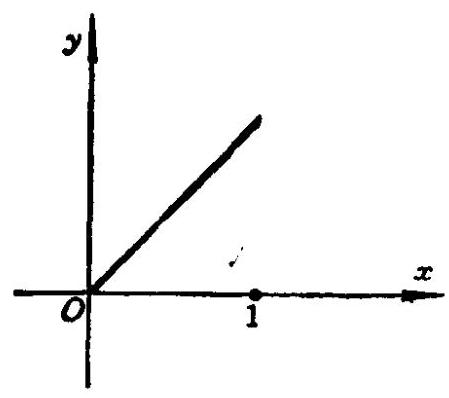
\includegraphics[max width=0.3\textwidth]{images/bo_d25ksc77aajc738obdgg_299_339_1662_449_398_0.jpg}
\end{center}
\hspace*{3em} 

图 6-5

\begin{center}
	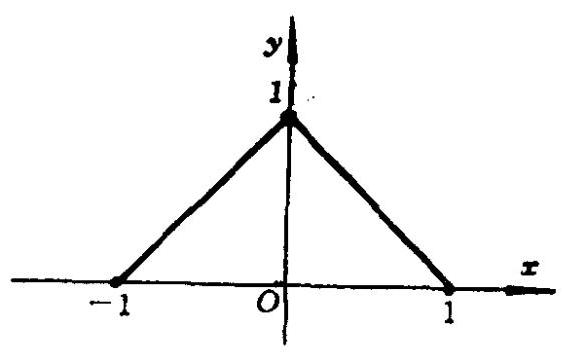
\includegraphics[max width=0.4\textwidth]{images/bo_d25ksc77aajc738obdgg_299_839_1680_562_354_0.jpg}
\end{center}
\hspace*{3em} 

图 6-6

例2 考虑函数
$$x \mapsto  f\left( x\right)  = \left\{  \begin{array}{ll} x + 1, &  - 1 \leq  x \leq  0; \\  1 - x, & 0 \leq  x \leq  1. \end{array}\right.$$

$f$ 在 $\left\lbrack  {-1,1}\right\rbrack$ 上连续, $f\left( {-1}\right)  = f\left( 1\right)  = 0$ ,但也不存在 $\xi  \in  \rbrack  - 1,1\lbrack$ 使得 ${f}^{\prime }\left( \xi \right)  = 0$ 。原因是 $f$ 在 $x = 0$ 处不可导.

例 3 考虑函数 $x \mapsto  f\left( x\right)  = x,x \in  \left\lbrack  {0,1}\right\rbrack$ .

$f$ 在 $\left\lbrack  {0,1}\right\rbrack$ 上连续, $f$ 在 $\rbrack 0,1\lbrack$ 上可导,但同样不存在 $\xi  \in  \rbrack 0,1\lbrack$ 使得 ${f}^{\prime }\left( \xi \right)  = 0$ ,这是因为 $f\left( 0\right)  = f\left( 1\right)$ .

当然也有这样的函数 $f : \left\lbrack  {a,b}\right\rbrack   \rightarrow  \mathbf{R}$ ,它不满足 Rolle 定理中的任一个条件, 但 Rolle 定理的结论仍然成立. 因此 Rolle 定理的条件是充分的而不是必要的.

例4 考虑函数
$$x \mapsto  f\left( x\right)  = \left\{  \begin{array}{ll} x, & 0 \leq  x \leq  1; \\  2, & 1 < x \leq  2. \end{array}\right.$$

\begin{center}
	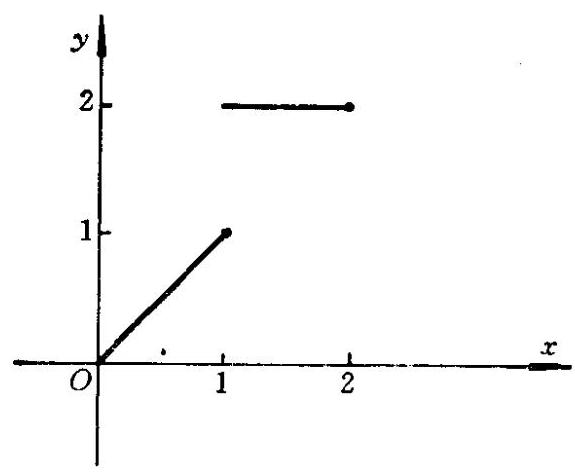
\includegraphics[max width=0.5\textwidth]{images/bo_d25ksc77aajc738obdgg_300_390_1388_575_474_0.jpg}
\end{center}
\hspace*{3em} 

图 6-7

$f$ 在 $x = 1$ 处不连续,当然 $f$ 在 $x = 1$ 处不可导,并且 $f\left( 0\right)  \neq  f\left( 2\right)$ . 然而 $\forall \xi  \in  \rbrack 1,2\left\lbrack  {,{f}^{\prime }\left( \xi \right)  = 0}\right.$ .

Rolle定理的几何意义十分明显. 如果连续函数 $f : \left\lbrack  {a,b}\right\rbrack   \rightarrow$ R在 $\rbrack a,b\lbrack$ 上可导,并且 $f\left( a\right)  = f\left( b\right)$ ,则在函数 $f$ 所表示的曲线 $\Gamma$ 上至少存在一点 ${M}_{0}\left( {\xi ,f\left( \xi \right) }\right) \left( {\xi  \in  \rbrack a,b\lbrack }\right)$ ,使得 $\Gamma$ 在点 ${M}_{0}$ 处的切线 $T$ 平行于 $x$ 轴.

\begin{center}
	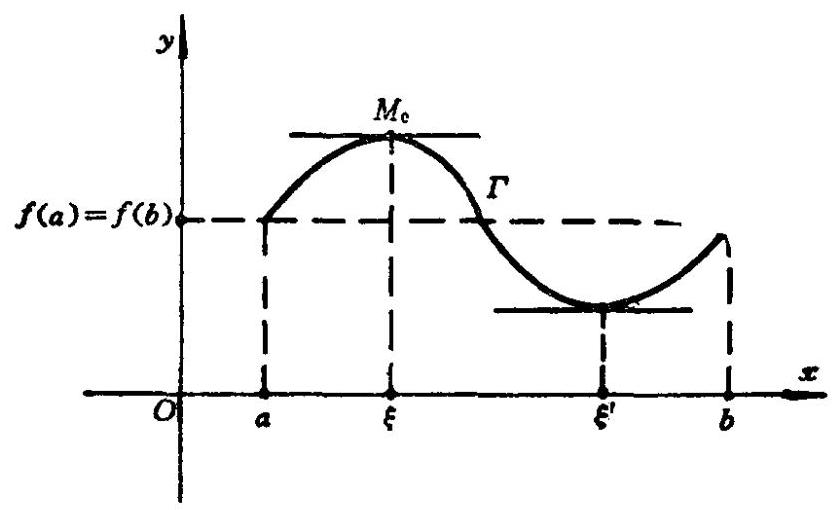
\includegraphics[max width=0.7\textwidth]{images/bo_d25ksc77aajc738obdgg_301_473_490_833_510_0.jpg}
\end{center}
\hspace*{3em} 

图 6-8

\section*{2. Lagrange 中值定理}

定理 $6 \cdot  3 \cdot  2$ (Lagrange中值定理) 设 $\left\lbrack  {a,b}\right\rbrack$ 是任一有限闭区间, $f : \left\lbrack  {a,b}\right\rbrack   \rightarrow  \mathbf{R}$ 是任一函数,满足下述条件:

1) $f$ 在 $\left\lbrack  {a,b}\right\rbrack$ 上连续,

$2)f$ 在 $\rbrack a,b\lbrack$ 上可导,

则存在一点 $\xi  \in  \rbrack a,b\lbrack$ 使得
$$f\left( b\right)  - f\left( a\right)  = {f}^{\prime }\left( \xi \right) \left( {b - a}\right) .$$

证明 考虑辅助函数 $F : \left\lbrack  {a,b}\right\rbrack   \rightarrow  \mathbf{R}$
$$F\left( x\right)  = f\left( x\right)  - \left\lbrack  {f\left( a\right)  + \frac{f\left( b\right)  - f\left( a\right) }{b - a}\left( {x - a}\right) }\right\rbrack  ,x \in  \left\lbrack  {a,b}\right\rbrack  .$$

显然 $F$ 在 $\left\lbrack  {a,b}\right\rbrack$ 上连续,在 $\rbrack a,b\lbrack$ 上可导,并且 $F\left( a\right)  = F\left( b\right)$ . 根据Rolle定理,存在一点 $\xi  \in  \rbrack a,b\lbrack$ 使得 ${F}^{\prime }\left( \xi \right)  = 0$ . 此即为
$${f}^{\prime }\left( \xi \right)  = \frac{f\left( b\right)  - f\left( a\right) }{b - a}\text{ 或 }f\left( b\right)  - f\left( a\right)  = {f}^{\prime }\left( \xi \right) \left( {b - a}\right) .$$

Lagrange中值定理的几何解释是: 如果 $\Gamma$ 是函数 $f$ 所表示的曲线,则在 $\Gamma$ 上存在一点 ${M}_{0}\left( {\xi ,f\left( \xi \right) }\right)$ ,它异于 $\Gamma$ 的两个端点 $A\left( {a,f\left( a\right) }\right) \text{ 、 }B\left( {b,f\left( b\right) }\right)$ ,使得 $\Gamma$ 在点 ${M}_{0}$ 处的切线平行于联结点 $A$ 与 $B$ 的直线.

\begin{center}
	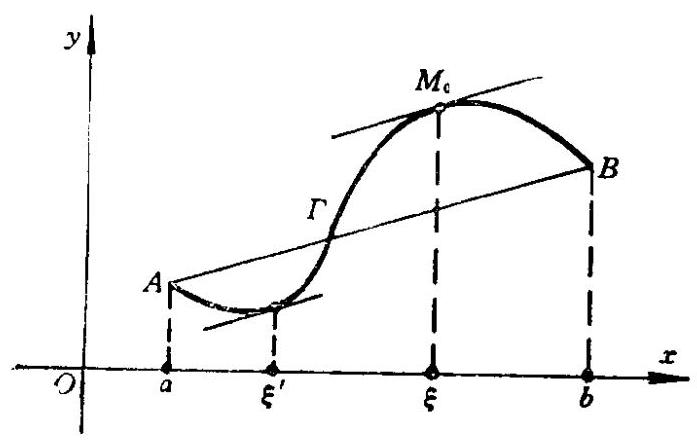
\includegraphics[max width=0.6\textwidth]{images/bo_d25ksc77aajc738obdgg_302_343_516_697_444_0.jpg}
\end{center}
\hspace*{3em} 

图 6-9

作为Lagrange 中值定理的一个应用, 我们来证明下述重要命题.

命题 假设 $I \subset  \mathbf{R}$ 是一区间,函数 $f : I \rightarrow  \mathbf{R}$ 在 $I$ 上可导. 则 $f$ 在 $I$ 上为常值函数的充分必要条件是:
$${f}^{\prime }\left( x\right)  = 0,\;\forall x \in  I.$$

证明 必要性 设 $f = c\left( {c \in  \mathbf{R}}\right)$ ,则显然有 ${f}^{\prime }\left( x\right)  = 0,\forall x \in$  $I$ .

充分性 设 ${f}^{\prime }\left( x\right)  = 0,\forall x \in  I$ 。我们证明 $f$ 在 $I$ 上为常值函数. 为此只需证明
$$\forall {x}_{1},{x}_{2} \in  I\text{ 且 }{x}_{1} \neq  {x}_{2},f\left( {x}_{1}\right)  = f\left( {x}_{2}\right) \text{ . }$$

事实上,不妨假设 ${x}_{1} < {x}_{2}$ ,由于 $f$ 在 $\left\lbrack  {{x}_{1},{x}_{2}}\right\rbrack$ 上可导,故由 Lagrange中值定理知,存在 $\xi  \in  \rbrack {x}_{1},{x}_{2}\lbrack$ 使得
$$f\left( {x}_{2}\right)  - f\left( {x}_{1}\right)  = {f}^{\prime }\left( \xi \right) \left( {{x}_{2} - {x}_{1}}\right) .$$

但 ${f}^{\prime }\left( \xi \right)  = 0$ ,因此 $f\left( {x}_{2}\right)  - f\left( {x}_{1}\right)  = 0$ ,即 $f\left( {x}_{1}\right)  = f\left( {x}_{2}\right)$ .

推论 $I$ 如上所述. $f : I \rightarrow  \mathbf{R}$ 与 $g : I \rightarrow  \mathbf{R}$ 是任意两个在 $I$ 上可导的函数, 并且满足
$${f}^{\prime }\left( x\right)  = {g}^{\prime }\left( x\right) ,\forall x \in  I.$$

则存在常数 $c$ 使得
$$f\left( x\right)  - g\left( x\right)  = c,\;\forall x \in  I.$$

证明 因为 ${f}^{\prime }\left( x\right)  = {g}^{\prime }\left( x\right) ,\forall x \in  I$ ,所以 ${\left\lbrack  f\left( x\right)  - g\left( x\right) \right\rbrack  }^{\prime } =$  $0,\forall x \in  I$ ,从而由上述命题知,存在常数 $c$ 使得
$$f\left( x\right)  - g\left( x\right)  = c,\;\forall x \in  I.$$

\section*{3. Cauchy 中值定理}

定理 $6 \cdot  3 \cdot  3$ (Cauchy中值定理) 设 $\left\lbrack  {a,b}\right\rbrack$ 是任一有限闭区间. $f,g : \left\lbrack  {a,b}\right\rbrack   \rightarrow  \mathbf{R}$ 是任意两个函数,满足下述条件:

1) $f,g$ 在 $\left\lbrack  {a,b}\right\rbrack$ 上连续,

2) $f,g$ 在 $\rbrack a,b\lbrack$ 上可导,

3) ${g}^{\prime }\left( x\right)  \neq  0,\forall x \in  \rbrack a,b\lbrack$ .

则存在一点 $\xi  \in  \rbrack a,b\lbrack$ 使得
$$\frac{f\left( b\right)  - f\left( a\right) }{g\left( b\right)  - g\left( a\right) } = \frac{{f}^{\prime }\left( \xi \right) }{{g}^{\prime }\left( \xi \right) }.$$

证明 首先我们注意到 $g\left( b\right)  - g\left( a\right)  \neq  0$ . 因为若 $g\left( b\right)$  $- g\left( a\right)  = 0$ ,则由 Rolle 定理知,存在 $\bar{x} \in  \rbrack a,b\lbrack$ ,使得 ${g}^{\prime }\left( \bar{x}\right)  =$ 0, 这与条件 3 ) 相矛盾.

现在作辅助函数 $F : \left\lbrack  {a,b}\right\rbrack   \rightarrow  \mathbf{R}$ :
\begin{align*}
	&F\left( x\right)  = f\left( x\right)  - \left\lbrack  {f\left( a\right)  + \frac{f\left( b\right)  - f\left( a\right) }{g\left( b\right)  - g\left( a\right) }\left( {g\left( x\right)  - g\left( a\right) }\right) }\right\rbrack  ,\\
	&\forall x \in  \left\lbrack  {a,b}\right\rbrack  \text{ . }
\end{align*}

则 $F$ 在 $\left\lbrack  {a,b}\right\rbrack$ 上连续, $F$ 在 $\rbrack a,b\lbrack$ 上可导,并且 $F\left( a\right)  = F\left( b\right)$ . 因此由Rolle定理知,存在一点 $\xi  \in  \rbrack a,b\lbrack$ 使得 ${F}^{\prime }\left( \xi \right)  = 0$ ,此即为

$0 = {f}^{\prime }\left( \xi \right)  - \frac{f\left( b\right)  - f\left( a\right) }{g\left( b\right)  - g\left( a\right) }{g}^{\prime }\left( \xi \right)$ 或 $\frac{f\left( b\right)  - f\left( a\right) }{g\left( b\right)  - g\left( a\right) } = \frac{{f}^{\prime }\left( \xi \right) }{{g}^{\prime }\left( \xi \right) }.$

关于 Cauchy 中值定理, 我们作以下几点说明.

附注 1 若 $g\left( x\right)  = x,\forall x \in  \left\lbrack  {a,b}\right\rbrack$ ,则 Cauchy 中值定理的结论化为
$$\frac{f\left( b\right)  - f\left( a\right) }{b - a} = {f}^{\prime }\left( \xi \right) ,\xi  \in  \rbrack a,b\lbrack .$$

这正是 Lagrange 中值定理的结论。因此 Cauchy 中值定理是 Lagrange中值定理的推广.

2) 若我们分别对函数 $f,g$ 应用Lagrange中值定理,则我们只能得到下述形式的等式:
$$\frac{f\left( b\right)  - f\left( a\right) }{g\left( b\right)  - g\left( a\right) } = \frac{{f}^{\prime }\left( {\xi }_{1}\right) \left( {b - a}\right) }{{g}^{\prime }\left( {\xi }_{2}\right) \left( {b - a}\right) } = \frac{{f}^{\prime }\left( {\xi }_{1}\right) }{{g}^{\prime }\left( {\xi }_{2}\right) },{\xi }_{1},{\xi }_{2} \in  \rbrack a,b\lbrack .$$

这里 ${\xi }_{1},{\xi }_{2}$ 不一定相等. 因此我们不能得到 Cauchy 中值定理中所要求的等式.

3) 若我们在 Cauchy 中值定理中删去条件 3 ), 则有下述对称形式的等式成立:
$$\left\lbrack  {f\left( b\right)  - f\left( a\right) }\right\rbrack  {g}^{\prime }\left( \xi \right)  = \left\lbrack  {g\left( b\right)  - g\left( a\right) }\right\rbrack  {f}^{\prime }\left( \xi \right) ,\xi  \in  \rbrack a,b\lbrack .$$

这是因为,若 $g\left( b\right)  - g\left( a\right)  = 0$ ,则由 Rolle 定理知存在一点 $\xi  \in  \rbrack a,b\lbrack$ ,使得 ${g}^{\prime }\left( \xi \right)  = 0$ ,从而
$$\left\lbrack  {f\left( b\right)  - f\left( a\right) }\right\rbrack  {g}^{\prime }\left( \xi \right)  = 0 = \left\lbrack  {g\left( b\right)  - g\left( a\right) }\right\rbrack  {f}^{\prime }\left( \xi \right) .$$

若 $g\left( b\right)  - g\left( a\right)  \neq  0$ ,则只需重复 Cauchy 中值定理的证明, 由 $0 = {f}^{\prime }\left( \xi \right)  - \frac{f\left( b\right)  - f\left( a\right) }{g\left( b\right)  - g\left( a\right) }{g}^{\prime }\left( \xi \right)$ 两边同乘以 $g\left( b\right)  - g\left( a\right)$ 即可.

\section*{4. Darboux定理}

定理 $6 \cdot  3 \cdot  4$ (Darboux定理) 设 $I \subset  \mathrm{R}$ 是任一区间, $f : I \rightarrow$  $\mathrm{R}$ 是任一在 $I$ 上可导的函数,则 ${f}^{\prime }\left( I\right)  \subset  \mathrm{R}$ 也是一区间.

证明 为了证明 ${f}^{\prime }\left( I\right)  \subset  \mathbf{R}$ 是区间,我们只需证明:
$$\forall y,z \in  {f}^{\prime }\left( I\right) \text{ 且 }y < z \Rightarrow  \rbrack y,z\lbrack  \subset  {f}^{\prime }\left( I\right) .$$

为此设 $a,b \in  I$ 使得 ${f}^{\prime }\left( a\right)  = y,{f}^{\prime }\left( b\right)  = z$ ,不妨假设 $a < b$ . 任取 $\omega  \in  \rbrack y,z\lbrack$ ,我们来证明至少存在一点 $\xi  \in  \rbrack a,b\lbrack$ 使得 ${f}^{\prime }\left( \xi \right)  =$ 0 .

为了书写简单起见,我们就记 $f$ 为 $f$ 在区间 $\left\lbrack  {a,b}\right\rbrack$ 上的限制 $f{|}_{\left\lbrack  a;b\right\rbrack  }$ . 考虑辅助函数
$$F : \left\lbrack  {a,b}\right\rbrack   \rightarrow  \mathbf{R},\forall x \in  \left\lbrack  {a,b}\right\rbrack  ,F\left( x\right)  = f\left( x\right)  - {\omega x}.$$

函数 $F$ 在 $\left\lbrack  {a,b}\right\rbrack$ 上连续,并且可导. 根据连续函数性质知, $F$ 在 $\left\lbrack  {a,b}\right\rbrack$ 上达到它的最小值.

显然 $F$ 不可能在 $a$ 与 $b$ 处取到其最小值. 否则
\begin{align*}
	&{F}^{\prime }\left( a\right)  = \mathop{\lim }\limits_{{x \rightarrow  {a}^{ + }}}\frac{F\left( x\right)  - F\left( a\right) }{x - a} \geq  0,{F}^{\prime }\left( b\right)  = \mathop{\lim }\limits_{{x \rightarrow  {b}^{ - }}}\frac{F\left( x\right)  - F\left( b\right) }{x - b}.\\
	&\leq  0,
\end{align*}

这与 ${F}^{\prime }\left( a\right)  = {f}^{\prime }\left( a\right)  - \omega  < 0,{F}^{\prime }\left( b\right)  = {f}^{\prime }\left( b\right)  - \omega  > 0$ ,相矛盾.

因此存在一内点 $\xi  \in  \rbrack a,b\lbrack$ 使得 $F\left( \xi \right)$ 为 $F$ 在 $\left\lbrack  {a,b}\right\rbrack$ 上的最小值. 于是
$${F}^{\prime }\left( \xi \right)  = \mathop{\lim }\limits_{{x \rightarrow  {\xi }^{ + }}}\frac{F\left( x\right)  - F\left( \xi \right) }{x - \xi } \geq  0,{F}^{\prime }\left( \xi \right)  = \mathop{\lim }\limits_{{x \rightarrow  {\xi }^{ - }}}\frac{F\left( x\right)  - F\left( \xi \right) }{x - \xi }$$

从而 ${F}^{\prime }\left( \xi \right)  = 0$ 即 ${f}^{\prime }\left( \xi \right)  = \omega$ 或 $\omega  \in  {f}^{\prime }\left( I\right)$ .

由 $\omega  \in  \rbrack y,z\lbrack$ 的任意性知, $\rbrack y,z\lbrack  \subset  {f}^{\prime }\left( I\right)$ . 因此 ${f}^{\prime }\left( I\right)  \subset  \mathbf{R}$ 是一区间.

推论 设 $I \subset  \mathbf{R}$ 是任一区间. 若函数 $f : I \rightarrow  \mathbf{R}$ 在 $I$ 上可导,并且 $\forall x \in  I,{f}^{\prime }\left( x\right)  \neq  0$ ,则
$$\forall x \in  I,{f}^{\prime }\left( x\right)  > 0\text{ 或 }\forall x \in  I,{f}^{\prime }\left( {x}^{\prime }\right)  < 0.$$

\section*{习 题}

1. 设函数 $f,g : \left\lbrack  {a,b}\right\rbrack   \rightarrow  R$ 满足下述条件:

1) $f,g$ 在 $\left\lbrack  {a,b}\right\rbrack$ 上连续.

2) $f,g$ 在 $\rbrack a,b\lbrack$ 上可导,并且 ${\left( {f}^{\prime }\right) }^{2} + {\left( {g}^{\prime }\right) }^{2} \neq  0$ .

3) $g\left( a\right)  \neq  g\left( b\right)$ .

证明: 存在 $\xi  \in  \rbrack a,b\lbrack$ 使得
$$\frac{f\left( b\right)  - f\left( a\right) }{g\left( b\right)  - g\left( a\right) } = \frac{{f}^{\prime }\left( \xi \right) }{{g}^{\prime }\left( \xi \right) }.$$

2. 设函数 $f,g : \left\lbrack  {a,b}\right\rbrack   \rightarrow  \mathrm{R}$ 满足下述条件:

1) $f,g$ 在 $\left\lbrack  {a,b}\right\rbrack$ 上连续.

2) $f,g$ 在 $\rbrack a,b\lbrack$ 上可导,并且 ${g}^{\prime } \neq  0$ .

证明: 存在 $\xi  \in  \rbrack a,b\lbrack$ 使得
$$\frac{f\left( \xi \right)  - f\left( a\right) }{g\left( b\right)  - g\left( \xi \right) } = \frac{{f}^{\prime }\left( \xi \right) }{{g}^{\prime }\left( \xi \right) }.$$

3. 设函数 $f,g,h : \left\lbrack  {a,b}\right\rbrack   \rightarrow  \mathrm{R}$ 满足下述条件:

1) $f,g,h$ 在 $\left\lbrack  {a,b}\right\rbrack$ 上连续.

2) $f,g,h$ 在 $\rbrack a,b\lbrack$ 上可导.

证明: 存在 $\xi  \in  \rbrack a,b\lbrack$ 使得
$$\left| \begin{array}{lll} f\left( a\right) & f\left( b\right) & {f}^{\prime }\left( \xi \right) \\  g\left( a\right) & g\left( b\right) & {g}^{\prime }\left( \xi \right) \\  h\left( a\right) & h\left( b\right) & {h}^{\prime }\left( \xi \right)  \end{array}\right|  = 0.$$

4. 证明: 在 ${e}^{x}\sin x = 1$ 的两个实根中至少存在 ${e}^{x}\cos x =  - 1$ 的一个实根.

5. 设 $f : \left\lbrack  {a,b}\right\rbrack   \rightarrow  \mathrm{R}$ 是任一函数. $\alpha  > 0$ . 我们称 $f$ 是 $\alpha$ 次Lipschitz函数, 如果存在 $k > 0$ 使得
$$\left| {f\left( x\right)  - f\left( y\right) }\right|  \leq  k{\left| x - y\right| }^{a},\;\forall x,y \in  \left\lbrack  {a,b}\right\rbrack  .$$

1) 证明: 若 $f$ 在 $\left\lbrack  {a,b}\right\rbrack$ 上是连续可导的,则 $f$ 是 1 次 Lipschitz函数。

2) 证明: 若 $f$ 在 $\left\lbrack  {a,b}\right\rbrack$ 上是可导的 1 次 Lipschitz函数,则 ${f}^{\prime }$ 在 $\left\lbrack  {a,b}\right\rbrack$ 上有界.

3) 证明: 若 $f$ 是 $\alpha  > 1$ 次 Lipschitz 函数,则 $f$ 在 $\left\lbrack  {a,b}\right\rbrack$ 上为常值函数.

6. 设 $f : R \rightarrow  R$ 是任一在 $R$ 上可导的函数,并且 $\mathop{\lim }\limits_{{x \rightarrow   + \infty }}f\left( x\right)  = \mathop{\lim }\limits_{{x \rightarrow   - \infty }}f\left( x\right)$ (有限或正负无穷大). 证明: 存在 $\xi  \in  \mathrm{R}$ 使得 ${f}^{\prime }\left( \xi \right)  = 0$ .

7. 设 $a \in  R,f : \lbrack a, + \infty \lbrack$ 是任一函数,满足条件:

1) $f$ 在 $\lbrack a, + \infty \lbrack$ 上连续,

2) $f$ 在 $\rbrack a, + \infty \lbrack$ 上可导,

3) $\mathop{\lim }\limits_{{x \rightarrow   + \infty }}f\left( x\right)  = f\left( a\right)$ .

证明: 存在 $\xi  \in  \rbrack a, + \infty \lbrack$ 使得 ${f}^{\prime }\left( \xi \right)  = 0$ .

8. 设 $\left\lbrack  {a,b}\right\rbrack   \subset  R,f : \left\lbrack  {a,b}\right\rbrack   \rightarrow  R$ 满足下述条件:

1) $f$ 在 $\left\lbrack  {a,b}\right\rbrack$ 上连续,

2) $f$ 在 $\rbrack a,b\lbrack$ 上可导,

3) $\mathop{\lim }\limits_{{x \rightarrow  {a}^{ + }}}f\left( x\right)  = \mathop{\lim }\limits_{{x \rightarrow  {b}^{ - }}}f\left( x\right)  =  + \infty$ .

证明: $\forall A \in  R$ ,存在 $\xi  \in  \rbrack a,b\lbrack$ 使得 ${f}^{\prime }\left( \xi \right)  = A$ .

9. 设 $a \in  R,h > 0$ ,函数 $f : \left\lbrack  {a,a + {2h}}\right\rbrack   \rightarrow  R$ 在 $\left\lbrack  {a,a + {2h}}\right\rbrack$ 上 2 次可导. 证明: 存在 $\theta  \in  \rbrack 0,1\lbrack$ 使得
$$f\left( a\right)  - {2f}\left( {a + h}\right)  + f\left( {a + {2h}}\right)  = {h}^{2}{f}^{\prime \prime }\left( {a + {2\theta h}}\right) .$$

10. 设 $a,b \in  \mathrm{R}\left\lbrack  {\left| {a < b,f : }\right| a,b}\right\rbrack   \rightarrow  \mathrm{R}$ 是任一在 $\rbrack a,b\lbrack$ 上可导的函数. 假设 $\mathop{\lim }\limits_{{x \rightarrow  {x}^{ - }}}f\left( x\right)  =  + \infty$ . 证明: 若 ${f}^{\prime }$ 在 $\rbrack a,b\lbrack$ 上单调上升,则 $\mathop{\lim }\limits_{{x \rightarrow  {b}^{ - }}}{f}^{\prime }\left( x\right)  =$  $+ \infty$ ; 若 ${f}^{\prime }$ 不是单调上升的,则 $\mathop{\lim }\limits_{{x \rightarrow  {b}^{ - }}}{f}^{\prime }\left( x\right)  =  + \infty$ 可以不成立.

11. 设函数 $f : \left\lbrack  {a,b}\right\rbrack   \rightarrow  R$ 在 $\left\lbrack  {a,b}\right\rbrack$ 上可导. 证明: 存在一点 $\xi  \in  \rbrack a,b\lbrack$ 使得
$$f\left( \xi \right)  - \xi {f}^{\prime }\left( \xi \right)  = \frac{1}{a - b}\left| \begin{array}{ll} a & b \\  f\left( a\right) & f\left( b\right)  \end{array}\right| .$$

12. 设函数 $f : \left\lbrack  {-a,a}\right\rbrack   \rightarrow  R$ 在 $\rbrack  - a,a\lbrack$ 上 $n$ 次可导,并且 ${f}^{\left( k\right) }\left( 0\right)  = 0$  $\left( {k = 0,1,\cdots ,n - 1}\right)$ . 证明: $\forall x \in  \rbrack  - a,a\lbrack$ 且 $x \neq  0$ ,存在 $0 < \theta  < 1$ 使得
$$\frac{f\left( x\right) }{{x}^{n}} = \frac{{f}^{\left( n\right) }\left( {\theta x}\right) }{n!}$$

13. 设函数 $f : \left\lbrack  {a,b}\right\rbrack   \rightarrow  \mathrm{R}$ 在 $\rbrack a,b\lbrack$ 上 $n + 1$ 次可导,并且 ${f}^{\left( k\right) }\left( a\right)  =$  ${f}^{\left( k\right) }\left( b\right)  = 0\left( {k = 0,1,\cdots ,n}\right)$ 。证明: 存在 $\xi  \in  \rbrack a,b\lbrack$ 使得 ${f}^{\left( n + 1\right) }\left( \xi \right)  =$  $f\left( \xi \right)$ .

14. 设 $f : \rbrack a,b\lbrack  \rightarrow  R$ 是任一在 $\rbrack a,b\lbrack$ 上可导的函数. 并且 $f$ 的零点集至少有一个聚点 $\left. {{a}_{0} \in  }\right\rbrack  a,b\lbrack$ .

1) 证明: ${f}^{\prime }\left( {a}_{0}\right)  = 0$ ,并且 ${f}^{\prime }$ 的零点集也有聚点 ${a}_{0}$ .

2) 若 $f$ 在 $\rbrack a,b\lbrack$ 上 $p$ 次可导 $\left( {p \geq  1}\right)$ ,证明: $f$ 的各阶导函数 ${f}^{\left( k\right) }(k =$  $1,2,\cdots ,p)$ 都以 ${a}_{0}$ 为其零点.

3) 证明: 不存在任何的多项式函数使得它与函数 $x \mapsto  {e}^{x}$ 在 $R$ 的任何无限点集 $A$ 上取相同的值.

15. 设 $- \infty  < {a}_{1} < {a}_{2} < \cdots  < {a}_{n} <  + \infty ,f : \left\lbrack  {{a}_{1},{a}_{n}}\right\rbrack   \rightarrow  R$ 在 $\left\lbrack  {{a}_{1},{a}_{n}}\right\rbrack$ 上是 ${C}^{n - 1}$ 类的 $\left( {n \geq  2}\right)$ . 在 $\rbrack {a}_{1},{a}_{n}\lbrack$ 上有 $n$ 阶导数,并且 $f\left( {a}_{i}\right)  = 0,i = 1,2$ , $\cdots ,n$ . 证明:
\begin{align*}
	&\left( {\forall x \in  \left\lbrack  {{a}_{1},{a}_{n}}\right\rbrack  }\right) \left( {\exists \xi  \in  \rbrack {a}_{1},{a}_{n}\lbrack }\right) \text{ 使得 }\\
	&f\left( x\right)  = \frac{\left( {x - {a}_{1}}\right) \left( {x - {a}_{2}}\right) \cdots \left( {x - {a}_{n}}\right) }{n!}{f}^{\left( n\right) }\left( \xi \right) .
\end{align*}

16. 设 $f : \left\lbrack  {a,b}\right\rbrack   \rightarrow  \mathrm{R}$ 在 $\left\lbrack  {a,b}\right\rbrack$ 上可导, ${f}^{\prime } : \left\lbrack  {a,b}\right\rbrack   \rightarrow  \mathrm{R}$ 在 $\left\lbrack  {a,b}\right\rbrack$ 上可积, 令
$${\delta }_{n} = {\int }_{a}^{b}f\left( x\right) {dx} - \mathop{\sum }\limits_{{k = 1}}^{n}\frac{b - a}{n}f\left( {a + k\frac{b - a}{n}}\right) ,$$

试计算极限 $\mathop{\lim }\limits_{{n \rightarrow   + \infty }}{\delta }_{n}$ .

\section{导数的应用}

函数导数的应用是多方面的, 下面我们介绍它的三个方面的应用.

\section*{1. 函数单调性的研究}

定理 $6 \cdot  4 \cdot  1$ 设 $I \subset  \mathbf{R}$ 是任一区间. $f : I \rightarrow  \mathbf{R}$ 是任一在 $I$ 上可导的函数, 则下述结论成立:

1) $f$ 在 $I$ 上单调上升 (下降) $\Leftrightarrow  \forall x \in  I,{f}^{\prime }\left( x\right)  \geq  0\left( { \leq  0}\right)$ .

2) $f$ 在 $I$ 上严格单调上升 (下降),若 $\forall x \in  I,{f}^{\prime }\left( x\right)  > 0$  $\left( { < 0}\right)$ .

证明 我们只对上升情形进行证明. 下降情形的证明完全类似.

设 ${x}_{1},{x}_{2} \in  I$ 且 ${x}_{1} < {x}_{2}$ . 由 Lagrange 中值定理,我们有

$f\left( {x}_{2}\right)  - f\left( {x}_{1}\right)  = {f}^{\prime }\left( \xi \right) \left( {{x}_{2} - {x}_{1}}\right) ,\xi  \in  \rbrack {x}_{1},{x}_{2}\lbrack .$(水)

1) 若 $f$ 在 $I$ 上单调上升,则 $f\left( {x}_{2}\right)  \geq  f\left( {x}_{1}\right)$ . 于是
$${f}^{\prime }\left( {x}_{1}\right)  = \mathop{\lim }\limits_{{{x}_{2} \rightarrow  {x}_{1}^{ + }}}\frac{f\left( {x}_{2}\right)  - f\left( {x}_{1}\right) }{{x}_{2} - {x}_{1}} \geq  0.$$

由 ${x}_{1} \in  I$ 的任意性知, $\forall x \in  I,{f}^{\prime }\left( x\right)  \geq  0$ .

反之若 $\forall x \in  I,{f}^{\prime }\left( x\right)  \geq  0$ ,则由 $\left( *\right)$ 知, $f\left( {x}_{2}\right)  \geq  f\left( {x}_{1}\right)$ ,从而 $f$ 在 $I$ 上单调上升.

2) 若 $\forall x \in  I,{f}^{\prime }\left( x\right)  > 0$ ,则由 (*) 式推出 $f\left( {x}_{2}\right)  > f\left( {x}_{1}\right)$ . 因此 $f$ 在 $I$ 上严格单调上升.

注意 即使 $f : I \rightarrow  \mathbf{R}$ 在 $I$ 上是严格单调上升的可导函数,也不一定有: $\forall x \in  I,{f}^{\prime }\left( x\right)  > 0$ .

为此,考虑函数 $x \mapsto  f\left( x\right)  = {x}^{3},x \in  \mathbf{R}$ .

因为 ${f}^{\prime }\left( x\right)  = 3{x}^{2} > 0,\forall x \in  \mathbf{R} - \{ 0\}$ . 所以 $f$ 在 $\rbrack  - \infty ,0\lbrack$ 与 ] $0, + \infty \lbrack$ 上是严格单调上升的. 并且
$${y}^{3} < 0 < {x}^{3},\;\forall x \in  \rbrack 0, + \infty \left\lbrack  {,\;\forall y \in  }\right\rbrack   - \infty ,0\lbrack .$$

故此函数 $f$ 在 $\mathbf{R}$ 上是严格单调上升的. 然而, ${f}^{\prime }\left( 0\right)  = 0$ . 下面我们举几个应用定理 $6 \cdot  4 \cdot  1$ 的例子. 例1 证明下述两个不等式成立: 1) $x < \operatorname{tg}x,\;\forall x \in  \rbrack 0,\frac{\pi }{2}\lbrack$ 2) $\frac{2}{\pi }x < \sin x < x,\;\forall x \in  \rbrack 0,\frac{\pi }{2}\lbrack$ . 为此我们定义
\begin{align*}
	&f\left( x\right)  = \operatorname{tg}x - x,\;\forall x \in  \left\lbrack  {0,\frac{\pi }{2}\lbrack ;}\right.\\
	&g\left( x\right)  = x - \sin x,\;\forall x \in  \left\lbrack  {0,\frac{\pi }{2}}\right\rbrack  ,\\
	&h\left( x\right)  = \left\{  \begin{array}{ll} \frac{\sin x}{x} - \frac{2}{\pi }, & \forall x \in  \rbrack 0,\frac{\pi }{2}\rbrack , \\  1 - \frac{2}{\pi }, & x = 0. \end{array}\right.
\end{align*}

显然我们只需证明: $f\left( x\right)  > 0,g\left( x\right)  > 0,h\left( x\right)  > 0,\forall x \in  \rbrack 0,\frac{\pi }{2}\lbrack$ . 对于 $f$ : 由于
$$\left. {{f}^{\prime }\left( x\right)  = \frac{1}{{\cos }^{2}x} - 1 = \frac{1 - {\cos }^{2}x}{{\cos }^{2}x} > 0,\forall x \in  }\right\rbrack  0,\frac{\pi }{2}\lbrack .$$

故 $\left. {f\text{ 在 }}\right\rbrack  0,\frac{\pi }{2}\lbrack$ 上是严格单调上升的. 而 $f\left( 0\right)  = 0$ ,因此 $f\left( x\right)  > 0$ .

$\left. {\forall x \in  }\right\rbrack  0,\frac{\pi }{2}\left\lbrack  {\text{ ,此即表示 }x < \operatorname{tg}x,\forall x \in  }\right\rbrack  0,\frac{\pi }{2}\lbrack$ .

对于 $g$ : 由于 ${g}^{\prime }\left( x\right)  = 1 - \cos x > 0,\forall x \in  \rbrack 0,\frac{\pi }{2}\lbrack$ ,故 $g$ 在 $\rbrack 0,\frac{\pi }{2}\lbrack$ 上是严格单调上升的,而 $g\left( 0\right)  = 0$ ,因此 $g\left( x\right)  > 0,\forall x \in$ ] $0,\frac{\pi }{2}\left\lbrack  {\text{ ,即 }\sin x < x,\forall x \in  }\right\rbrack  0,\frac{\pi }{2}\lbrack .$

对于 $h$ : 由于
$${h}^{\prime }\left( x\right)  = {\left( \frac{\sin x}{x}\right) }^{\prime } = \frac{\cos x\left( {x - \operatorname{tg}x}\right) }{{x}^{2}} < 0,\;\forall x \in  \rbrack 0,\frac{\pi }{2}\lbrack ,$$

故 $h$ 在 $\rbrack 0,\frac{\pi }{2}\lbrack$ 上是严格单调下降的,而 $h\left( \frac{\pi }{2}\right)  = 0$ ,因此 $h\left( x\right)  > 0$ , $\forall x \in  \rbrack 0,\frac{\pi }{2}\lbrack$ ,即
$$\left. {\frac{\sin x}{x} - \frac{2}{\pi } > 0\text{ 或 }\frac{2}{\pi }x < \sin x,\;\forall x \in  }\right\rbrack  0,\frac{\pi }{2}\lbrack .$$

结合对 $g$ 与 $h$ 的讨论,即证得
$$\left. {\frac{2}{\pi }x < \sin x < x,\;\forall x \in  }\right\rbrack  0,\frac{\pi }{2}\lbrack .$$

例 2 设函数 $f : \left\lbrack  {a, + \infty \left\lbrack  { \rightarrow  \mathbf{R}\left( {a \in  \mathbf{R}}\right) }\right. }\right.$ 满足条件:

1) $f$ 在 $\lbrack a, + \infty \lbrack$ 上可导且 $f\left( a\right)  < 0$ ,

2) 存在常数 $k > 0$ 使得 ${f}^{\prime }\left( x\right)  > k,\forall x \in  \rbrack a, + \infty \lbrack$ . 则方程 $\left. {f\left( x\right)  = 0\text{ 在开区间 }}\right\rbrack  a,a - \frac{f\left( a\right) }{k}\lbrack$ 上存在唯一的一个实根.

事实上,由 ${f}^{\prime }\left( x\right)  > 0,\forall x \in  \rbrack a, + \infty \left\lbrack  {\text{ ,故 }f}\right.$ 在 $\rbrack a, + \infty \lbrack$ 上是严格单调上升的. 由于 $f\left( a\right)  < 0$ ,若我们能证明 $\left. {f\left( {a - \frac{f\left( a\right) }{k}}\right)  > 0\text{ ,则由连续函数性质知,存在 唯一的 }\xi  \in  }\right\rbrack  a$ ,

$a - \frac{f\left( a\right) }{k}\left\lbrack  {\;\text{ 使得 }f\left( \xi \right)  = 0.}\right.$

为此我们注意到 $f$ 在 $\rbrack a, + \infty \lbrack$ 上可导,故由 Lagrange 中值定理得到
\begin{align*}
	&f\left( {a - \frac{f\left( a\right) }{k}}\right)  - f\left( a\right)  = {f}^{\prime }\left( \xi \right) \left\lbrack  {a - \frac{f\left( a\right) }{k} - a}\right\rbrack\\
	&= {f}^{\prime }\left( \xi \right)  \cdot  \left( {-\frac{f\left( a\right) }{k}}\right)\\
	&> k \cdot  \left( \frac{-f\left( a\right) }{k}\right)  =  - f\left( a\right) ,
\end{align*}

因此 $f\left( {a - \frac{f\left( a\right) }{k}}\right)  > 0$ .

例3 设函数 $f : \left\lbrack  {0,1}\right\rbrack   \rightarrow  \mathbf{R}$ 在 $\left\lbrack  {0,1}\right\rbrack$ 上连续,并且 $\left| {f\left( x\right) }\right|  <$ 1, $\forall x \in  \left\lbrack  {0,1}\right\rbrack$ . 证明: 方程 ${2x} - {\int }_{0}^{x}f\left( t\right) {dt} = 1$ 在 $\left\lbrack  {0,1}\right\rbrack$ 上存在唯一的解.

令 $F\left( x\right)  = {2x} - {\int }_{0}^{x}f\left( t\right) {dt} - 1,\forall x \in  \left\lbrack  {0,1}\right\rbrack$ . 则函数 $F : \left\lbrack  {0,1}\right\rbrack$  $\rightarrow  \mathrm{R}$ 在 $\left\lbrack  {0,1}\right\rbrack$ 上连续可导,并且
$${F}^{\prime }\left( x\right)  = 2 - f\left( x\right)  > 0,\;\forall x \in  \left\lbrack  {0,1}\right\rbrack  .$$

因此函数 $F$ 在 $\left\lbrack  {0,1}\right\rbrack$ 上严格单调上升. 由于
$$F\left( 0\right)  =  - 1 < 0,F\left( 1\right)  = 2 - {\int }_{0}^{1}f\left( t\right) {dt} - 1 > 0,$$

故存在唯一的 $\xi  \in  \rbrack 0$ , $1\lbrack$ 使得 $F\left( \xi \right)  = 0$ 。此即表明方程 ${2x} - {\int }_{0}^{x}f\left( t\right) {dt} = 1$ 在 $\left\lbrack  {0,1}\right\rbrack$ 上存在唯一的解.

\section*{2. 函数的凸凹性研究}

定义 设 $E \subset  {\mathbf{R}}^{2}$ 是任一非空集合. 我们称 $E$ 是凸的,若 $A$ 、

$E \in  E$ ,则连续 $A\text{ 、 }E$ 两点的线段 $\overline{AB} \subset  E$ .

现在我们设 $A = \left( {{x}_{1},{y}_{1}}\right) ,B = \left( {{x}_{2},{y}_{2}}\right)$ . 并规定:
\begin{align*}
	&\forall \alpha ,\beta  \in  \mathbf{R},{\alpha A} + {\beta B}\overset{ \bigtriangleup  }{ = }\alpha \left( {{x}_{1},{y}_{1}}\right)  + \beta \left( {{x}_{2},{y}_{2}}\right)\\
	&= \left( {\alpha {x}_{1} + \beta {x}_{2},\alpha {y}_{1} + \beta {y}_{2}}\right) ,
\end{align*}

则连结 $A$ 、 $B$ 两点的线段
\begin{align*}
	&\overline{AB} = \{ {\alpha A} + {\beta B} \mid  \alpha ,\beta  \in  \left\lbrack  {0,1}\right\rbrack  ,\alpha  + \beta  = 1\}\\
	&= \{ \left( {1 - t}\right) A + {tB} \mid  t \in  \left\lbrack  {0,1}\right\rbrack  \} .
\end{align*}

因此
\begin{align*}
	&E\text{ 是凸的 } \Leftrightarrow  \forall A\text{ 、 }B \in  E,\forall \alpha \text{ 、 }\beta  \in  \left\lbrack  {0,1}\right\rbrack  ,\alpha  + \beta  = 1\text{ , }\\
	&{\alpha A} + {\beta B} \in  E\\
	&\Leftrightarrow  \forall A\text{ 、 }B \in  E,\;\forall t \in  \left\lbrack  {0,1}\right\rbrack  ,\left( {1 - t}\right) A + {tB} \in  E.
\end{align*}

例4 平面上的三角形、长方形、圆盘、椭圆盘都是平面凸集, 而平面上的五角星不是平面凸集 (图 6-10).

\begin{center}
	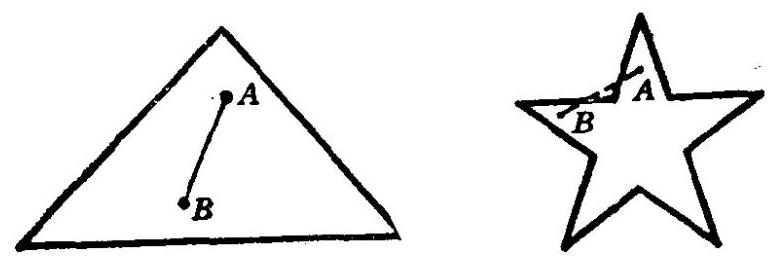
\includegraphics[max width=0.6\textwidth]{images/bo_d25ksc77aajc738obdgg_312_315_1171_774_265_0.jpg}
\end{center}
\hspace*{3em} 

图 6-10

\begin{center}
	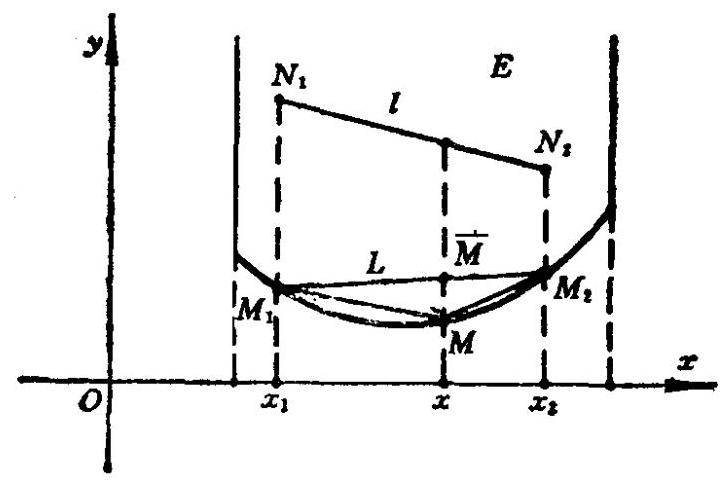
\includegraphics[max width=0.6\textwidth]{images/bo_d25ksc77aajc738obdgg_312_338_1561_726_483_0.jpg}
\end{center}
\hspace*{3em} 

图 6-11

设 $I \subset  \mathbf{R}$ 是任一区间, $f : I \rightarrow  \mathbf{R}$ 是任一函数. 我们定义下述集合
$$E = \left\{  {\left( {x,y}\right)  \in  {\mathbf{R}}^{2} \mid  x \in  I,y \geq  f\left( x\right) }\right\}  .$$

首先我们证明下述引理.

引理 设 $I \subset  \mathrm{R}$ 是任一区间, $f : I \rightarrow  \mathrm{R}$ 是任一函数,集 $E$ 如上所定义. 则下述三个结论互相等价:

1) $E$ 是凸集.

2) $\forall {x}_{1},{x}_{2} \in  I,\forall {\alpha }_{1},{\alpha }_{2} \in  \left\lbrack  {0,1}\right\rbrack$ 且 ${\alpha }_{1} + {\alpha }_{2} = 1$ ,
$$f\left( {{a}_{1}{x}_{1} + {a}_{2}{x}_{2}}\right)  \leq  {\alpha }_{1}f\left( {x}_{1}\right)  + {\alpha }_{2}f\left( {x}_{2}\right) .$$

3) $\forall {x}_{1},{x}_{2},x \in  I$ 且 ${x}_{1} < x < {x}_{2}$ ,
$$\frac{f\left( x\right)  - f\left( {x}_{1}\right) }{x - {x}_{1}} \leq  \frac{f\left( {x}_{2}\right)  - f\left( {x}_{1}\right) }{{x}_{2} - {x}_{1}} \leq  \frac{f\left( {x}_{2}\right)  - f\left( x\right) }{{x}_{2} - x}.$$

证明 $1) \Rightarrow  2$ ) 设 $E$ 是凸集. ${x}_{1},{x}_{2} \in  I,{x}_{1} \leq  {x}_{2},{\alpha }_{1}$ , ${\alpha }_{2} \in  \left\lbrack  {0,1}\right\rbrack$ 且 ${\alpha }_{1} + {\alpha }_{2} = 1$ . 那末 ${x}_{1} \leq  {\alpha }_{1}{x}_{1} + {\alpha }_{2}{x}_{2} \leq  {x}_{2}$ .

令 ${M}_{1} = \left( {{x}_{1},f\left( {x}_{1}\right) }\right) ,{M}_{2} = \left( {{x}_{2},f\left( {x}_{2}\right) }\right)$ ,则 ${M}_{1},{M}_{2}$ 是函数 $f$ 所表示的曲线 $\Gamma$ 上的两点. 因此 ${M}_{1},{M}_{2} \in  E$ .

连结 ${M}_{1}$ 与 ${M}_{2}$ 的直线段 $L$ 的方程为
$$y = f\left( {x}_{1}\right)  + \frac{f\left( {x}_{2}\right)  - f\left( {x}_{1}\right) }{{x}_{2} - {x}_{1}}\left( {x - {x}_{1}}\right) ,x \in  \left\lbrack  {{x}_{1},{x}_{2}}\right\rbrack  .$$

直接计算可知, $L$ 上对应于 $x = {\alpha }_{1}{x}_{1} + {\alpha }_{2}{x}_{2}$ 的点 $\bar{M}$ 为
\begin{align*}
	&\bar{M} = \left( {{\alpha }_{1}{x}_{1} + {\alpha }_{2}{x}_{2},{\alpha }_{1}f\left( {x}_{1}\right)  + {\alpha }_{2}f\left( {x}_{2}\right) }\right)\\
	&= {\alpha }_{1}\left( {{x}_{1},f\left( {x}_{1}\right) }\right)  + {\alpha }_{2}\left( {{x}_{2},f\left( {x}_{2}\right) }\right)\\
	&= {\alpha }_{1}{M}_{1} + {\alpha }_{2}{M}_{2},
\end{align*}

由于 $E$ 是凸的,故 $\bar{M} \in  E$ ,此即表明
$$f\left( {{\alpha }_{1}{x}_{1} + {\alpha }_{2}{x}_{2}}\right)  \leq  {\alpha }_{1}f\left( {x}_{1}\right)  + {\alpha }_{2}f\left( {x}_{2}\right) .$$

$2) \Rightarrow  3)$ 假设 2 )成立,并且 ${x}_{1},{x}_{2},x \in  I,{x}_{1} < x <$  ${x}_{2}$ . 于是存在 $t \in  \rbrack 0,1\lbrack$ 使得 $x = \left( {1 - t}\right) {x}_{1} + t{x}_{2}$ . 由此得到 $t =$  $\frac{x - {x}_{1}}{{x}_{2} - {x}_{1}}$ . 根据假设,我们有
\begin{align*}
	&f\left( x\right)  = f\left( {\left( {1 - t}\right) {x}_{1} + t{x}_{2}}\right)  \leq  \left( {1 - i}\right) f\left( {x}_{1}\right)  + {tf}\left( {x}_{2}\right)\\
	&= \frac{{x}_{2} - x}{{x}_{2} - {x}_{1}}f\left( {x}_{1}\right)  + \frac{x - {x}_{1}}{{x}_{2} - {x}_{1}}f\left( {x}_{2}\right) ,
\end{align*}

因此
\begin{align*}
	&f\left( x\right)  - f\left( {x}_{1}\right)  \leq  \left( {\frac{{x}_{2} - x}{{x}_{2} - {x}_{1}} - 1}\right) f\left( {x}_{1}\right)  + \frac{x - {x}_{1}}{{x}_{2} - {x}_{1}}f\left( {x}_{2}\right)\\
	&= \frac{x - {x}_{1}}{{x}_{2} - {x}_{1}}\left\lbrack  {f\left( {x}_{2}\right)  - f\left( {x}_{1}\right) }\right\rbrack  ,\\
	&f\left( {x}_{2}\right)  - f\left( x\right)  \geq  f\left( {x}_{2}\right)  - \frac{{x}_{2} - x}{{x}_{2} - {x}_{1}}f\left( {x}_{1}\right)  - \frac{x - {x}_{1}}{{x}_{2} - {x}_{1}}f\left( {x}_{2}\right)\\
	&=  - \frac{{x}_{2} - x}{{x}_{2} - {x}_{1}}f\left( {x}_{1}\right)  + \left( {1 - \frac{x - {x}_{1}}{{x}_{2} - {x}_{1}}}\right) f\left( {x}_{2}\right)\\
	&= \frac{{x}_{2} - x}{{x}_{2} - {x}_{1}}\left\lbrack  {f\left( {x}_{2}\right)  - f\left( {x}_{1}\right) }\right\rbrack  .
\end{align*}

由这两个不等式立即推得
$$\frac{f\left( x\right)  - f\left( {x}_{1}\right) }{x - {x}_{1}} \leq  \frac{f\left( {x}_{2}\right)  - f\left( {x}_{1}\right) }{{x}_{2} - {x}_{1}} \leq  \frac{f\left( {x}_{2}\right)  - f\left( x\right) }{{x}_{2} - x}.$$

$3) \Rightarrow  1)$ 设 ${N}_{1} = \left( {{x}_{1},{y}_{1}}\right) ,{N}_{2} = \left( {{x}_{2},{y}_{2}}\right)  \in  E$ 。我们证明: 连结 ${N}_{1}\text{ 、 }{N}_{2}$ 两点的直线段 $l$ 位于 $E$ 内.

由 $E$ 的定义知, ${y}_{1} \geq  f\left( {x}_{1}\right) ,{y}_{2} \geq  f\left( {x}_{2}\right)$ . 因此连结点 ${M}_{1} = \left( {x}_{1}\right.$ , $\left. {f\left( {x}_{1}\right) }\right)$ 与点 ${M}_{2} = \left( {{x}_{2},f\left( {x}_{2}\right) }\right)$ 的直线段 $L$ 位于直线段 $l$ 的下方 (如图 6-11 所示). 为了证明 $l$ 位于 $E$ 内,我们只需证明 $L$ 位于 $E$ 内即可.

事实上,由假设对 ${x}_{1},{x}_{2},x \in  I$ 且 ${x}_{1} < x < {x}_{2}$ 成立不等式
$$\frac{f\left( x\right)  - f\left( {x}_{1}\right) }{x - {x}_{1}} \leq  \frac{f\left( {x}_{2}\right)  - f\left( {x}_{1}\right) }{{x}_{2} - {x}_{1}} \leq  \frac{f\left( {x}_{2}\right)  - f\left( x\right) }{{x}_{2} - x},$$

故由左边不等式得到
$$f\left( {x}_{1}\right)  + \frac{f\left( {x}_{2}\right)  - f\left( {x}_{1}\right) }{{x}_{2} - {x}_{1}}\left( {x - {x}_{1}}\right)  \geq  f\left( x\right) ,$$

此即表明点 $\left( {x,f\left( {x}_{1}\right)  + \frac{f\left( {x}_{2}\right)  - f\left( {x}_{1}\right) }{{x}_{2} - {x}_{1}}\left( {x - {x}_{1}}\right) }\right)  \in  E$ ,而这一点正好是直线段 $L$ 上的点,由 $x \in  \rbrack {x}_{1},{x}_{2}\lbrack$ 的任意性知, $L$ 整个地位于 $E$ 内。因此 $E$ 是凸集. 图

根据上述引理, 现在我们可以给出关于凸函数的下述定义.

定义 设 $I \subset  \mathbf{R}$ 是任一区间, $f : I \rightarrow  \mathbf{R}$ 是任一函数.

1)我们称 $f$ 是凸的,如果
\begin{align*}
	&\forall {x}_{1},{x}_{2} \in  I,\forall {a}_{1},{\alpha }_{2} \in  \left\lbrack  {0,1}\right\rbrack  \text{ 且 }{\alpha }_{1} + {\alpha }_{2} = 1\\
	&\Rightarrow  f\left( {{a}_{1}{x}_{1} + {a}_{2}{x}_{2}}\right)  \leq  {a}_{1}f\left( {x}_{1}\right)  + {a}_{2}f\left( {x}_{2}\right) .
\end{align*}

2) 我们称 $f$ 是凹的,如果函数 $- f$ 是凸的.

例 5 函数 $x \mapsto  {x}^{2},x \in  \mathrm{R}$ 是凸的.

事实上,设 ${x}_{1},{x}_{2} \in  \mathbf{R},{\alpha }_{1},{\alpha }_{2} \in  \left\lbrack  {0,1}\right\rbrack$ 且 ${\alpha }_{1} + {\alpha }_{2} = 1$ ,则
\begin{align*}
	&{\left( {\alpha }_{1}{x}_{1} + {\alpha }_{2}{x}_{2}\right) }^{2} = {\alpha }_{1}^{2}{x}_{1}^{2} + {\alpha }_{2}^{2}{x}_{2}^{2} + 2{\alpha }_{1}{\alpha }_{2}{x}_{1}{x}_{2}\\
	&\leq  {\alpha }_{1}^{2}{x}_{1}^{2} + {\alpha }_{2}^{2}{x}_{2}^{2} + {\alpha }_{1}{\alpha }_{2}\left( {{x}_{1}^{2} + {x}_{2}^{2}}\right)\\
	&= \left( {{\alpha }_{1}^{2} + {\alpha }_{1}{\alpha }_{2}}\right) {x}_{1}^{2} + \left( {{\alpha }_{2}^{2} + {\alpha }_{1}{\alpha }_{2}}\right) {x}_{2}^{2}\\
	&= {\alpha }_{1}\left( {{\alpha }_{1} + {\alpha }_{2}}\right) {x}_{1}^{2} + {\alpha }_{2}\left( {{\alpha }_{1} + {\alpha }_{2}}\right) {x}_{2}^{2}\\
	&= {\alpha }_{1}{x}_{1}^{2} + {\alpha }_{2}{x}_{2}^{2}.
\end{align*}

因此函数 $x \mapsto  {x}^{2},x \in  \mathbf{R}$ 是凸的.

下面我们给出凸函数的另一个等价定义即Jensen不等式, 它本身也有其重要的应用价值.

定理 $6 \cdot  4 \cdot  2$ (Jensen不等式) 函数 $f : I \rightarrow  \mathrm{R}$ 是凸的,当且仅当: $\forall {x}_{i} \in  I,\forall {\alpha }_{i} \in  \left\lbrack  {0,1}\right\rbrack  \left( {i = 1,2,\cdots ,n}\right)$ 且 $\mathop{\sum }\limits_{{i = 1}}^{n}{\alpha }_{i} = 1$ 有
\begin{align*}
	&f\left( {{\alpha }_{1}{x}_{1} + {\alpha }_{2}{x}_{2} + \cdots  + {\alpha }_{n}{x}_{n}}\right)  \leq  {\alpha }_{1}f\left( {x}_{1}\right)  + {\alpha }_{2}f\left( {x}_{2}\right)  + \cdots\\
	&+ {\alpha }_{n}f\left( {x}_{n}\right) \text{ . }
\end{align*}
(*)

证明 若不等式 $\left( *\right)$ 成立,则取 $n = 2$ 时表明 $f$ 是凸的.

反之,设 $f$ 是凸的. 我们对 $n$ 用数学归纳法证明.

当 $n = 2$ 时,不等式 (*) 即为凸函数的定义.

现在假设 $n = k$ 时不等式 (*) 成立. 我们来证明不等式 (*) 对 $n = k + 1$ 也成立.

设 ${x}_{1},{x}_{2},\cdots ,{x}_{k},{x}_{k + 1} \in  I,{\alpha }_{1},{\alpha }_{2},\cdots ,{\alpha }_{k},{\alpha }_{k + 1} \in  \lbrack 0$ ,

1]并且 ${\alpha }_{1} + {\alpha }_{2} + \cdots  + {\alpha }_{k} + {\alpha }_{k + 1} = 1$ . 不失一般性,可以假设
$${\alpha }_{1} + {\alpha }_{2} + \cdots  + {\alpha }_{k} = 0。$$

于是由归纳法假设我们有
\begin{align*}
	&f\left( {\frac{{\alpha }_{1}}{{\alpha }_{1} + \cdots  + {\alpha }_{k}}{x}_{1} + \cdots  + \frac{{\alpha }_{k}}{{\alpha }_{1} + \cdots  + {\alpha }_{k}}{x}_{k}}\right)\\
	&\leq  \mathop{\sum }\limits_{{i = 1}}^{k}\frac{{\alpha }_{i}}{{\alpha }_{1} + \cdots  + {\alpha }_{k}}f\left( {x}_{i}\right) ,
\end{align*}

因此
\begin{align*}
	&f\left( {{\alpha }_{1}{x}_{1} + \cdots  + {\alpha }_{k}{x}_{k} + {\alpha }_{k + 1}{x}_{k + 1}}\right)\\
	&= f\left\lbrack  {\left( {{\alpha }_{1} + \cdots  + {\alpha }_{k}}\right) \left( {\frac{{\alpha }_{1}}{{\alpha }_{1} + \cdots  + {\alpha }_{k}}{x}_{1} + \cdots }\right. }\right.\\
	&\left. {\left. {+\frac{{\alpha }_{k}}{{\alpha }_{1} + \cdots  + {\alpha }_{k}}{x}_{k}}\right)  + {\alpha }_{k + 1}{x}_{k + 1}}\right\rbrack\\
	&\leq  \left( {{\alpha }_{1} + \cdots  + {\alpha }_{k}}\right) f\left( {\frac{{\alpha }_{1}}{{\alpha }_{1} + \cdots  + {\alpha }_{k}}{x}_{1} + \cdots }\right.\\
	&\left. {+\frac{{\alpha }_{k}}{{\alpha }_{1} + \cdots  + {\alpha }_{k}}{x}_{k}}\right)  + {\alpha }_{k + 1}f\left( {x}_{k + 1}\right)\\
	&\leq  \left( {{\alpha }_{1} + \cdots  + {\alpha }_{k}}\right) \left\lbrack  {\frac{{\alpha }_{1}}{{\alpha }_{1} + \cdots  + {\alpha }_{k}}f\left( {x}_{1}\right)  + \cdots }\right.\\
	&\left. {+\frac{{\alpha }_{k}}{{\alpha }_{1} + \cdots  + {\alpha }_{k}}f\left( {x}_{k}\right) }\right\rbrack   + {\alpha }_{k + 1}f\left( {x}_{k + 1}\right)\\
	&= {\alpha }_{1}f\left( {x}_{1}\right)  + \cdots  + {\alpha }_{k}f\left( {x}_{k}\right)  + {\alpha }_{k + 1}f\left( {x}_{k + 1}\right) .
\end{align*}

此即表明不等式 (*) 对 $n = k + 1$ 成立. 因此由数学归纳 法知不等式 $\left( *\right)$ 对任意的 $n \in  \mathbf{N}$ 都成立. 目

作为Jensen 不等式的应用, 我们来证明下面几个重要不等式.

重要不等式 设 ${a}_{1},{a}_{2},\cdots ,{a}_{n},{b}_{1},{b}_{2},\cdots ,{b}_{n}$ 是任意 ${2n}$ 个非零实数, $p > 0,q > 0$ .

1) 若 ${a}_{i} > 0\left( {i = 1,2,\cdots ,n}\right)$ ,则
$$\frac{n}{\frac{1}{{a}_{1}} + \frac{1}{{a}_{2}} + \cdots  + \frac{1}{{a}_{n}}} \leq  \sqrt[n]{{a}_{1}{a}_{2}\cdots {a}_{n}} \leq  \frac{{a}_{1} + {a}_{2} + \cdots  + {a}_{n}}{n};$$

2) 若 $\frac{1}{p} + \frac{1}{q} = 1$ ,则下述Hölder不等式成立:
$$\mathop{\sum }\limits_{{i = 1}}^{n}\left| {{a}_{i}{b}_{i}}\right|  \leq  {\left( \mathop{\sum }\limits_{{i = 1}}^{n}{\left| {a}_{i}\right| }^{p}\right) }^{\frac{1}{p}}{\left( \mathop{\sum }\limits_{{i = 1}}^{n}{\left| {b}_{i}\right| }^{q}\right) }^{\frac{1}{q}},$$

3) 若 $p > 1$ ,则下述 Minkowski 不等式成立:
$${\left( \mathop{\sum }\limits_{{i = 1}}^{n}{\left| {a}_{i} + {b}_{i}\right| }^{p}\right) }^{\frac{1}{p}} \leq  {\left( \mathop{\sum }\limits_{{i = 1}}^{n}{\left| {a}_{i}\right| }^{p}\right) }^{\frac{1}{p}} + {\left( \mathop{\sum }\limits_{{i = 1}}^{n}{\left| {b}_{i}\right| }^{p}\right) }^{\frac{1}{p}}.$$

证明 1) 因为自然对数函数 $x \mapsto  \log x,x \in  {\mathbf{R}}_{ * }^{ + }$ 是 凹的 (*), 故 $\forall {a}_{i} > 0,{\alpha }_{i} \geq  0\left( {i = 1,2,\cdots ,n}\right)$ 且 ${\alpha }_{1} + {\alpha }_{2} + \cdots  + {\alpha }_{n} = 1$ ,由 Jensen不等式我们有
\begin{align*}
	&{\alpha }_{1}\log {a}_{1} + {\alpha }_{2}\log {a}_{2} + \cdots  + {\alpha }_{n}\log {a}_{n} \leq  \log \left( {{\alpha }_{1}{a}_{1} + {\alpha }_{2}{a}_{2} + \cdots }\right.\\
	&\left. {+{\alpha }_{n}{a}_{n}}\right) \text{ . }
\end{align*}

此即为
$${a}_{1}{a}_{1}{a}_{2}{a}_{2}\cdots {a}_{n}{a}_{n} \leq  {a}_{1}{a}_{1} + {a}_{2}{a}_{2} + \cdots  + {a}_{n}{a}_{n}.$$

若特别取 ${\alpha }_{1} = {\alpha }_{2} = \cdots  = {\alpha }_{n} = \frac{1}{n}$ ,则上述不等式就是
$$\sqrt[n]{{a}_{1}{a}_{2}\cdots {a}_{n}} \leq  \frac{{a}_{1} + {a}_{2} + \cdots  + {a}_{n}}{n}.$$

利用此不等式我们得到
$$\frac{n}{\frac{1}{{a}_{1}} + \frac{1}{{a}_{2}} + \cdots  + \frac{1}{{a}_{n}}} = \frac{1}{\frac{1}{{a}_{1}} + \frac{1}{{a}_{2}} + \cdots  + \frac{1}{{a}_{n}}} \leq  \frac{1}{\sqrt[n]{\frac{1}{{a}_{1}}\frac{1}{{a}_{2}}\cdots \frac{1}{{a}_{n}}}} = \sqrt[n]{{a}_{1}{a}_{2}\cdots {a}_{n}}$$

因此
$$\frac{n}{\frac{1}{{a}_{1}} + \frac{1}{{a}_{2}} + \cdots  + \frac{1}{{a}_{n}}} \leq  \sqrt[n]{{a}_{1}{a}_{2}\cdots {a}_{n}} \leq  \frac{{a}_{1} + {a}_{2} + \cdots  + {a}_{n}}{n}.$$

\footnote{
	
	① 这里我们可以先从它们的几何图形看出它们的凸凹性, 严格证明见例6.
	
}

2) 因为 $p > 0,q > 0$ 且 $\frac{1}{p} + \frac{1}{q} = 1$ ,所以 $p > 1$ . 由于幂函数 $x \mapsto  {x}^{p},x \in  {\mathbf{R}}_{ * }^{ + }$ 是凸函数 ①,故 $\forall {x}_{i} > 0,{a}_{i} \geq  0\left( {i = 1,2,\cdots ,n}\right)$ 且 ${\alpha }_{1} + {\alpha }_{2} + \cdots  + {\alpha }_{n} = 1$ ,由Jensen不等式有
$${\left( \mathop{\sum }\limits_{{i = 1}}^{n}\alpha  \cdot  {x}_{i}\right) }^{p} \leq  \mathop{\sum }\limits_{{i = 1}}^{n}{\alpha }_{i}{x}_{i}^{p}.$$

现在根据假设 $\forall i = 1,2,\cdots ,n,{a}_{i} \neq  0,{b}_{i} \neq  0$ 。我们可取
\begin{align*}
	&{x}_{i} = \frac{\left| {a}_{i}\right| \left( {{\left| {b}_{1}\right| }^{q} + {\left| {b}_{2}\right| }^{q} + \cdots  + {\left| {b}_{n}\right| }^{q}}\right) }{{\left| {b}_{i}\right| }^{\frac{1}{p - 1}}},\\
	&{\alpha }_{i} = \frac{{\left| {b}_{i}\right| }^{q}}{{\left| {b}_{1}\right| }^{q} + {\left| {b}_{2}\right| }^{q} + \cdots  + {\left| {b}_{n}\right| }^{q}},\\
	&\left( {i = 1,2,\cdots n}\right)
\end{align*}

由于 $q = \frac{p}{p - 1}$ ,故我们得到
\begin{align*}
	&{\left( \mathop{\sum }\limits_{{i = 1}}^{n}\left| {a}_{i}{b}_{i}\right| \right) }^{p} \leq  \mathop{\sum }\limits_{{i = 1}}^{n}{\left| {b}_{i}\right| }^{q - \frac{p}{p - 1}} \cdot  {\left| {a}_{i}\right| }^{p} \cdot  {\left( \mathop{\sum }\limits_{{i = 1}}^{n}{\left| {b}_{i}\right| }^{q}\right) }^{p - 1}\\
	&= \left( {\mathop{\sum }\limits_{{i = 1}}^{n}{\left| {a}_{i}\right| }^{p}}\right)  \cdot  {\left( \mathop{\sum }\limits_{{i = 1}}^{n}{\left| {b}_{i}\right| }^{q}\right) }^{p - 1},
\end{align*}

或
$$\mathop{\sum }\limits_{{i = 1}}^{n}\left| {{a}_{i}{b}_{i}}\right|  \leq  {\left( \mathop{\sum }\limits_{{i = 1}}^{n}{\left| {a}_{i}\right| }^{p}\right) }^{\frac{1}{p}} \cdot  {\left( \mathop{\sum }\limits_{{i = 1}}^{n}{\left| {b}_{i}\right| }^{q}\right) }^{\frac{1}{q}}.$$

3)首先我们有恒等式
\begin{align*}
	&\mathop{\sum }\limits_{{i = 1}}^{n}{\left( \left| {a}_{i}\right|  + \left| {b}_{i}\right| \right) }^{p} = \mathop{\sum }\limits_{{i = 1}}^{n}\left| {a}_{i}\right| {\left( \left| {a}_{i}\right|  + \left| {b}_{i}\right| \right) }^{p - 1}\\
	&+ \mathop{\sum }\limits_{{i = 1}}^{n}\left| {b}_{i}\right| {\left( \left| {a}_{i}\right|  + \left| {b}_{i}\right| \right) }^{p - i}
\end{align*}

\footnote{
	
	① 这里我们可以先从它们的几何图形看出它们的凸凹性:严格证明见例6.
	
}

对右边两项分别应用Hölder 不等式得到
\begin{align*}
	&\mathop{\sum }\limits_{{i = 1}}^{n}\left| {a}_{i}\right| {\left( \left| {a}_{i}\right|  + \left| {b}_{i}\right| \right) }^{p - 1} \leq  {\left( \mathop{\sum }\limits_{{i = 1}}^{n}{\left| {a}_{i}\right| }^{p}\right) }^{\frac{1}{p}}\\
	&\times  {\left( \mathop{\sum }\limits_{{i = 1}}^{n}{\left( \left| {a}_{i}\right|  + \left| {b}_{i}\right| \right) }^{q \cdot  p - 1}\right) }^{\frac{1}{q}},\\
	&\mathop{\sum }\limits_{{i = 1}}^{n}\left| {b}_{i}\right| {\left( \left| {a}_{i}\right|  + \left| {b}_{i}\right| \right) }^{p - 1} \leq  {\left( \mathop{\sum }\limits_{{i = 1}}^{n}{\left| {b}_{i}\right| }^{p}\right) }^{\frac{1}{p}}\\
	&\times  {\left( \mathop{\sum }\limits_{{i = 1}}^{n}{\left( \left| {a}_{i}\right|  + \left| {b}_{i}\right| \right) }^{q\left( {p - 1}\right) }\right) }^{\frac{1}{q}}.
\end{align*}

将它们代入上述恒等式的右边得
\begin{align*}
	&\mathop{\sum }\limits_{{i = 1}}^{n}{\left( \left| {a}_{i}\right|  + \left| {b}_{i}\right| \right) }^{p} \leq  \left\lbrack  {\left( \mathop{\sum }\limits_{{i = 1}}^{n}{\left| {a}_{i}\right| }^{p}\right) }^{\frac{1}{p}}\right.\\
	&\left. {+{\left( \mathop{\sum }\limits_{{i = 1}}^{n}{\left| {b}_{i}\right| }^{p}\right) }^{\frac{1}{p}}}\right\rbrack  {\left( \mathop{\sum }\limits_{{i = 1}}^{n}{\left( \left| {a}_{i}\right|  + \left| {b}_{i}\right| \right) }^{p}\right) }^{\frac{1}{q}}.
\end{align*}

两边再除去 ${\left( \mathop{\sum }\limits_{{i = 1}}^{n}{\left( \left| {a}_{i}\right|  + \left| {b}_{i}\right| \right) }^{p}\right) }^{\frac{1}{q}}$ 即得到
$${\left( \mathop{\sum }\limits_{{i = 1}}^{n}{\left( \left| {a}_{i}\right|  + \left| {b}_{i}\right| \right) }^{p}\right) }^{\frac{1}{p}} \leq  {\left( \mathop{\sum }\limits_{{i = 1}}^{n}{\left| {a}_{i}\right| }^{p}\right) }^{\frac{1}{p}} + {\left( \mathop{\sum }\limits_{{i = 1}}^{n}{\left| {b}_{i}\right| }^{p}\right) }^{\frac{1}{p}}.$$

最后由于 $\left| {{a}_{i} + {b}_{i}}\right|  \leq  \left| {a}_{i}\right|  + \left| {b}_{i}\right|$ ,故我们有
$${\left( \mathop{\sum }\limits_{{i = 1}}^{n}{\left| {a}_{i} + {b}_{i}\right| }^{p}\right) }^{\frac{1}{p}} \leq  {\left( \mathop{\sum }\limits_{{i = 1}}^{n}{\left| {a}_{i}\right| }^{p}\right) }^{\frac{1}{p}} + {\left( \mathop{\sum }\limits_{{i = 1}}^{n}{\left| {b}_{i}\right| }^{p}\right) }^{\frac{1}{p}}.$$

对于一个给定的函数 $f$ ,要从定义去判别它的凸凹性是比较困难的, 下面我们给出几个用起来比较方便的判别法则.

\section*{函数凸凹性判别法则}

首先我们介绍用导数判断函数凸凹性的定理.

定理 $6 \cdot  4 \cdot  3$ 设函数 $f : I \rightarrow  \mathbf{R}$ 在 $I$ 可导,则 $f$ 是凸 (凹) 的,当且仅当 $f$ 的导函数 ${f}^{\prime } : I \rightarrow  \mathrm{R}$ 在 $I$ 上是单调上升 (下降) 的.

证明 根据凹函数定义, 我们只需对凸函数进行证明.

设 $f$ 是凸的, ${x}_{1},{x}_{2} \in  I$ 且 ${x}_{1} < {x}_{2}$ . 根据上述引理, $\forall x \in$ ] ${x}_{1},{x}_{2}\lbrack$ ,有
$$\frac{f\left( x\right)  - f\left( {x}_{1}\right) }{x - {x}_{1}} \leq  \frac{f\left( {x}_{2}\right)  - f\left( {x}_{1}\right) }{{x}_{2} - {x}_{1}} \leq  \frac{f\left( {x}_{2}\right)  - f\left( x\right) }{{x}_{2} - x}.$$

由于 ${f}^{\prime }\left( {x}_{1}\right)$ 与 ${f}^{\prime }\left( {x}_{2}\right)$ 存在,故在上述不等式左端与右端先后令 $x \rightarrow  {x}_{1}^{ + }$ 与 $x \rightarrow  {x}_{2}^{ - }$ 得到
\begin{align*}
	&{f}^{\prime }\left( {x}_{1}\right)  = \mathop{\lim }\limits_{{x \rightarrow  {x}_{1}^{ + }}}\frac{f\left( x\right)  - f\left( {x}_{1}\right) }{x - {x}_{1}} \leq  \frac{f\left( {x}_{2}\right)  - f\left( {x}_{1}\right) }{{x}_{2} - {x}_{1}}\\
	&\leq  \mathop{\lim }\limits_{{x \rightarrow  {x}_{2}^{ - }}}\frac{f\left( {x}_{2}\right)  - f\left( x\right) }{{x}_{2} - x} = {f}^{\prime }\left( {x}_{2}\right) ,
\end{align*}

即
$${f}^{\prime }\left( {x}_{1}\right)  \leq  f\left( {x}_{2}^{\prime }\right) ,$$

因此 ${f}^{\prime }$ 在 $I$ 上单调上升.

反之设 ${f}^{\prime }$ 在 $I$ 上单调上升. ${x}_{1},{x}_{2} \in  I,{a}_{1},{a}_{2} \in  \left\lbrack  {0,1}\right\rbrack$ 且 ${a}_{1} +$  ${\alpha }_{2} = 1$ 。我们来证明
$$f\left( {{\alpha }_{1}{x}_{1} + {\alpha }_{2}{x}_{2}}\right)  \leq  {\alpha }_{1}f\left( {x}_{1}\right)  + {\alpha }_{2}f\left( {x}_{2}\right) .$$

不妨设 ${x}_{1} \leq  {x}_{2}$ . 由于 ${x}_{1} \leq  {\alpha }_{1}{x}_{1} + {\alpha }_{2}{x}_{2} \leq  {x}_{2}$ ,故由Lagrange中值定理有
\begin{align*}
	&f\left( {{\alpha }_{1}{x}_{1} + {\alpha }_{2}{x}_{2}}\right)  - f\left( {x}_{1}\right)  = {f}^{\prime }\left( \xi \right) \left( {{\alpha }_{1}{x}_{1} + {\alpha }_{2}{x}_{2} - {x}_{1}}\right)\\
	&= {\alpha }_{2}{f}^{\prime }\left( \xi \right) \left( {{x}_{2} - {x}_{1}}\right) ,\\
	&f\left( {x}_{2}\right)  - f\left( {{a}_{1}{x}_{1} + {a}_{2}{x}_{2}}\right)  = {f}^{\prime }\left( \eta \right) \left( {{x}_{2} - {a}_{1}{x}_{1} - {a}_{2}{x}_{2}}\right)\\
	&= {\alpha }_{1}{f}^{\prime }\left( \eta \right) \left( {{x}_{2} - {x}_{1}}\right) ,
\end{align*}

这里 ${x}_{1} \leq  \xi  \leq  {\alpha }_{1}{x}_{1} + {\alpha }_{2}{x}_{2} \leq  \eta  \leq  {x}_{2}$ . 由 ${f}^{\prime }$ 的单调上升性,有 ${f}^{\prime }\left( \xi \right)  \leq$  ${f}^{\prime }\left( \eta \right)$ ,从而
$${\alpha }_{1}\left\lbrack  {f\left( {{\alpha }_{1}{x}_{1} + {\alpha }_{2}{x}_{2}}\right)  - f\left( {x}_{1}\right) }\right\rbrack   - {\alpha }_{2}\left\lbrack  {f\left( {x}_{2}\right)  - f\left( {{\alpha }_{1}{x}_{1} + {\alpha }_{2}{x}_{2}}\right) }\right\rbrack   \leq  0,$$

或
$$f\left( {{\alpha }_{1}{x}_{1} + {\alpha }_{2}{x}_{2}}\right)  \leq  {\alpha }_{1}f\left( {x}_{1}\right)  + {\alpha }_{2}f\left( {x}_{2}\right) .$$

此即表明 $f$ 是凸的.

推论 若函数 $f : I \rightarrow  R$ 在 $I$ 上 2 次可导,则 $f$ 是凸 (四)的, 当且仅当 ${f}^{\prime \prime } \geq  0\left( { \leq  0}\right)$ .

例 6 证明: 自然对数函数 $x \mapsto  \log x,x \in  {\mathbf{R}}_{ * }^{ + }$ 是凹的,而 $\forall \alpha  > 1$ ,幂函数 $x \mapsto  {x}^{\alpha },x \in  {\mathbf{R}}_{ * }^{ + }$ 是凸的.

事实上,
$${\left( \log x\right) }^{\prime \prime } =  - \frac{1}{{x}^{2}} < 0,{\left( {x}^{a}\right) }^{\prime \prime } = \alpha \left( {\alpha  - 1}\right) {x}^{a - 2} > 0,\forall x \in  {\mathbf{R}}_{ * }^{ + }.$$

下面介绍用曲线的切线判断函数凸凹性的定理.

定理 $6 \cdot  4 \cdot  4$ 设函数 $f : I \rightarrow  \mathbf{R}$ 在 $I$ 上可导,则 $f$ 是凸 (凹)的,当且仅当函数 $f$ 的曲线 $\Gamma$ 不位于 $\Gamma$ 上任意一点 $M$ 的切线的下 (上) 方.

证明 我们只对凸性进行证明.

必要性 设 $f$ 是凸的. ${M}_{0} = \left( {{x}_{0},f\left( {x}_{0}\right) }\right)$ 是 $\Gamma$ 上任意固定一点. $\Gamma$ 在 ${M}_{0}$ 处的切线 $T$ 的方程为
$$y = y\left( x\right)  = f\left( {x}_{0}\right)  + {f}^{\prime }\left( {x}_{0}\right) \left( {x - {x}_{0}}\right) .$$

\begin{center}
	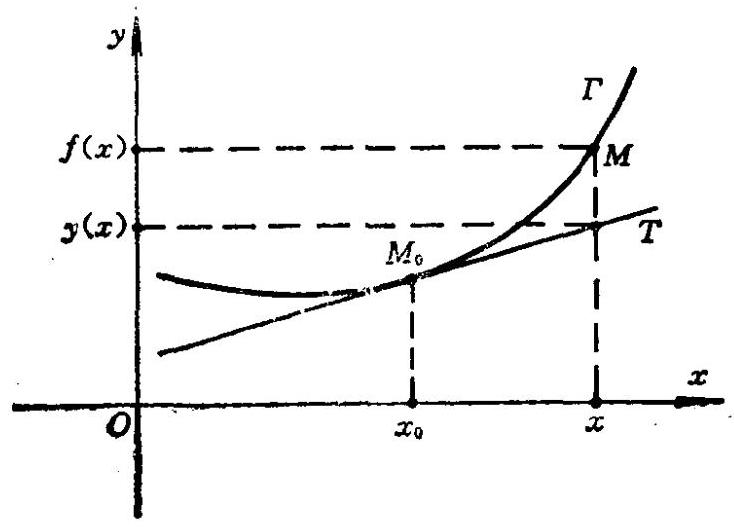
\includegraphics[max width=0.6\textwidth]{images/bo_d25ksc77aajc738obdgg_321_425_1246_734_528_0.jpg}
\end{center}
\hspace*{3em} 

图 6-12

为了证明 $\Gamma$ 上的任一点 $M = \left( {x,f\left( x\right) }\right)$ 不位于 $T$ 的下方,我们只需证明
$$f\left( x\right)  - y\left( x\right)  \geq  0,\;\forall x \in  I.$$

事实上, 由 Lagrange 中值定理, 我们有
\begin{align*}
	&f\left( x\right)  - y\left( x\right)  = f\left( x\right)  - f\left( {x}_{0}\right)  - {f}^{\prime }\left( {x}_{0}\right) \left( {x - {x}_{0}}\right)\\
	&= \left\lbrack  {{f}^{\prime }\left( \xi \right)  - {f}^{\prime }\left( {x}_{0}\right) }\right\rbrack  \left( {x - {x}_{0}}\right) ,
\end{align*}

这里 $\xi$ 介于 ${x}_{0}$ 与 $x$ 之间. 由于 $f$ 是凸的,根据定理 $6 \cdot  4 \cdot  3$ 知 ${f}^{\prime }$ 在 $I$ 上单调上升, 因此
$${f}^{\prime }\left( \xi \right)  - {f}^{\prime }\left( {x}_{0}\right) \left\{  \begin{array}{ll}  \geq  0, & \text{ 若 }x > {x}_{0}; \\   \leq  0, & \text{ 若 }x < {x}_{0}. \end{array}\right.$$

从而 $f\left( x\right)  - y\left( x\right)  \geq  0,\forall x \in  I$ .

充分性 假设定理的条件成立. 设 ${x}_{1},{x}_{2} \in  I,{\alpha }_{1},{\alpha }_{2} \in  \left\lbrack  {0,1}\right\rbrack$ 且 ${\alpha }_{1} + {\alpha }_{2} = 1$ . 不妨令 ${x}_{1} \leq  {x}_{2}$ . 于是 ${x}_{1} \leq  {\alpha }_{1}{x}_{1} + {\alpha }_{2}{x}_{2} \leq  {x}_{2}$ . 并且曲线 $\Gamma$ 不位于 $\Gamma$ 过点 $M = \left( {{\alpha }_{1}{x}_{1} + {\alpha }_{2}{x}_{2},f\left( {{\alpha }_{1}{x}_{1} + {\alpha }_{2}{x}_{2}}\right) }\right)$ 的切线 $T$ 的下方, 因此我们有
\begin{align*}
	&f\left( {x}_{1}\right)  - y\left( {x}_{1}\right)  = f\left( {x}_{1}\right)  - \left\lbrack  {f\left( {{\alpha }_{1}{x}_{1} + {\alpha }_{2}{x}_{2}}\right) }\right.\\
	&\left. {+{f}^{\prime }\left( {{a}_{1}{x}_{1} + {a}_{2}{x}_{2}}\right) \left( {{x}_{1} - {a}_{1}{x}_{1} - {a}_{2}{x}_{2}}\right) }\right\rbrack   \geq  0,\\
	&f\left( {x}_{2}\right)  - y\left( {x}_{2}\right)  = f\left( {x}_{2}\right)  - \left\lbrack  {f\left( {{a}_{1}{x}_{1} + {a}_{2}{x}_{2}}\right) }\right.\\
	&\left. {+{f}^{\prime }\left( {{\alpha }_{1}{x}_{1} + {\alpha }_{2}{x}_{2}}\right) \left( {{x}_{2} - {\alpha }_{1}{x}_{1} - {\alpha }_{2}{x}_{2}}\right) }\right\rbrack   \geq  0.
\end{align*}

由此得到
\begin{align*}
	&f\left( {x}_{1}\right)  - f\left( {{\alpha }_{1}{x}_{1} + {\alpha }_{2}{x}_{2}}\right)  \geq  {\alpha }_{2}{f}^{\prime }\left( {{\alpha }_{1}{x}_{1} + {\alpha }_{2}{x}_{2}}\right) \left( {{x}_{1} - {x}_{2}}\right) ,\\
	&f\left( {x}_{2}\right)  - f\left( {{\alpha }_{1}{x}_{1} + {\alpha }_{2}{x}_{2}}\right)  \geq  {\alpha }_{1}{f}^{\prime }\left( {{\alpha }_{1}{x}_{1} + {\alpha }_{2}{x}_{2}}\right) \left( {{x}_{2} - {x}_{1}}\right) .
\end{align*}

将第一个不等式乘以 ${\alpha }_{1}$ ,第二个不等式乘以 ${\alpha }_{2}$ 然后相加即得到
$$f\left( {{\alpha }_{1}{x}_{1} + {\alpha }_{2}{x}_{2}}\right)  \leq  {\alpha }_{1}f\left( {x}_{1}\right)  + {\alpha }_{2}f\left( {x}_{2}\right) .$$

因此 $f$ 是凸的.

例 7 考虑函数 $x \mapsto  f\left( x\right)  - {x}^{3},x \in  {\mathrm{R}}^{3}$ .

从图形上可以看出 $\forall x > 0$ ,函数 $f$ 的曲线 ${\Gamma }_{1}$ 位于过点 $M(x$ , $f\left( x\right) )$ 的切线 ${T}_{1}$ 的上方,而 $\forall x < 0$ ,函数 $f$ 的曲线 ${\Gamma }_{2}$ 位于过点 $M\left( {x,f\left( x\right) }\right)$ 的切线 ${T}_{2}$ 的下方. 因此 $f$ 在 $\rbrack 0, + \infty \lbrack$ 上是凸的,而 $f$ 在 $\rbrack  - \infty ,0\lbrack$ 上是凹的.

在原点(0,0)处函数 $f$ 的切线为 $x$ 轴. 因此 $f$ 的曲线 $\Gamma$ 穿过原

\begin{center}
	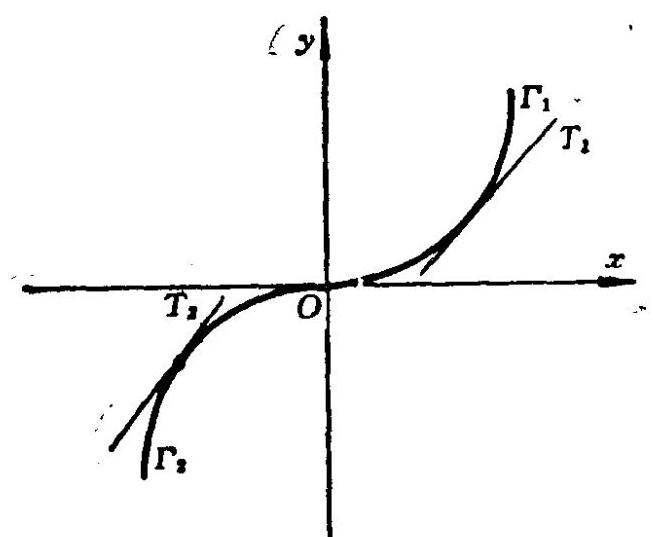
\includegraphics[max width=0.5\textwidth]{images/bo_d25ksc77aajc738obdgg_323_598_277_654_537_0.jpg}
\end{center}
\hspace*{3em} 

图 6-13

点时, $f$ 由凹变为凸. 函数 $f$ 的这种点值得我们注意,这就是下面介绍的拐点.

\section*{曲线的拐点}

定义 设 $I \subset  \mathbf{R}$ 是任一非空区间, $f : I \rightarrow  \mathbf{R}$ 是任一函数, $a \in  I$ 是一内点. 我们称 $a$ 是 $f$ 的拐点,如果存在 $\delta  > 0$ ,使得

1) $f$ 在 $\rbrack a - \delta ,a\lbrack$ 上的限制是凸 (凹)的,

2) $f$ 在 $\rbrack a,a + \delta \lbrack$ 上的限制是凹 (凸) 的.

通常我们称 $\left( {a,f\left( a\right) }\right)$ 是函数 $f$ 的曲线 $\Gamma$ 的拐点.

根据此定义知,函数 $x \mapsto  f\left( x\right)  = {x}^{3},x \in  \mathbf{R}$ 有唯一的拐点 0 .

\begin{center}
	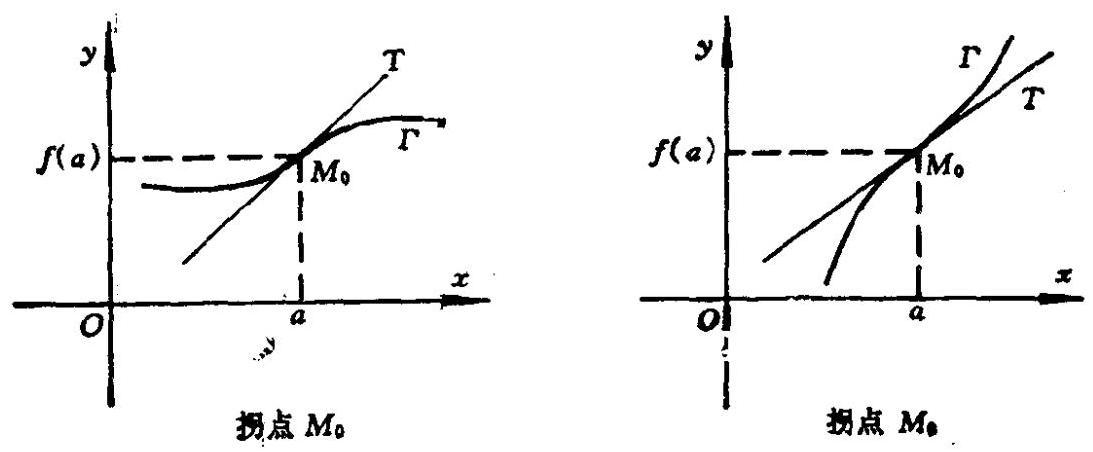
\includegraphics[max width=0.9\textwidth]{images/bo_d25ksc77aajc738obdgg_323_215_1535_1093_452_0.jpg}
\end{center}
\hspace*{3em} 

图 6-14

附注 从图 6-14 所示的在拐点 ${M}_{0}$ 的邻域内函数 $f$ 的图形 百出, $f$ 的曲线 $\Gamma$ 从拐点 ${M}_{0}$ 的切线的一侧穿到另一侧. 但必须注意, 曲线从某点的切线一侧穿到另一侧并不是拐点的充分条件. 我们可以构造出这样的函数 $f$ ,虽然 $f$ 的图形分别位于某点 ${M}_{0}$ 的切线的两侧,但在两侧 $f$ 并不保持确定的凸凹性.

例 8 考虑函数 $f : \mathbf{R} \rightarrow  \mathbf{R}$ ,它定义为
$$f\left( x\right)  = \left\{  \begin{matrix} {x}^{2}\left| {\sin \frac{\pi }{x}}\right| & , & x > 0; \\  0 & , & x = 0; \\   - {x}^{2}\left| {\sin \frac{\pi }{x}}\right| & , & x < 0. \end{matrix}\right.$$

它的图形如下图所示:

\begin{center}
	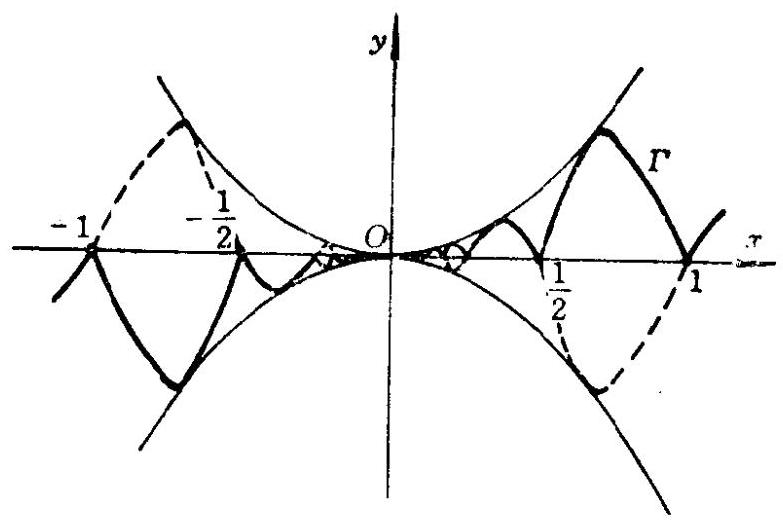
\includegraphics[max width=0.6\textwidth]{images/bo_d25ksc77aajc738obdgg_324_321_1026_783_521_0.jpg}
\end{center}
\hspace*{3em} 

图 6-15

此函数的曲线 $\Gamma$ 位于过原点的切线 (即 $x$ 轴) 的两侧,但原点并不是 $\Gamma$ 的拐点. 因为 $f$ 在 $x = 0$ 的任意右侧邻域与左侧邻域内都不保持凸凹性不变.

关于函数拐点的判别, 我们有下面的定理.

定理 $6 \cdot  4 \cdot  5$ 设 $f : I \rightarrow  R$ 是任一函数, $a \in  I$ 是一内点。

1) 若 $a$ 是 $f$ 的拐点,并且 ${f}^{\prime \prime }\left( a\right)$ 存在,则 ${f}^{\prime \prime }\left( a\right)  = 0$ .

2) 若存在 $\delta  > 0$ ,使得 $f$ 在 $\overset{ \circ  }{B}\left( {a,\delta }\right)$ 上 2 次可导,且
\begin{align*}
	&{f}^{\prime \prime }\left( x\right) \left\{  \begin{array}{ll}  > 0, & \forall x \in  {\overset{ \circ  }{B}}_{ + }\left( {a,\delta }\right) , \\   < 0, & \forall x \in  {\overset{ \circ  }{B}}_{ - }\left( {a,\delta }\right) ; \end{array}\right.\\
	&\text{ 或 }{f}^{\prime \prime }\left( x\right) \left\{  \begin{array}{ll}  < 0, & \forall x \in  \overset{ \circ  }{{B}_{ + }}\left( {a,\delta }\right) , \\   > 0, & \forall x \in  \overset{ \circ  }{{B}_{ - }}\left( {a,\delta }\right) . \end{array}\right.
\end{align*}

则 $a$ 是 $f$ 的拐点.

证明 1) 因为 ${f}^{\prime \prime }\left( a\right)$ 存在,所以存在 $\delta  > 0$ ,使得 ${f}^{\prime }$ 在 $\rbrack a -$  $\delta ,a + \delta \lbrack$ 上存在.

另一方面,由于 $a$ 是 $f$ 的拐点,故由定义知,只要 $\delta  > 0$ 充分小. $f$ 在 $\rbrack a - \delta ,a\lbrack$ 上是凸 (凹) 的,而在 $\rbrack a,a + \delta \lbrack$ 上 $f$ 是凹 (凸) 的,不妨设 $f$ 在 $\rbrack a - \delta ,a\lbrack$ 上是凸的,而 $f$ 在 $\rbrack a,a + \delta \lbrack$ 上是凹的,于是根据定理 $6 \cdot  4 \cdot  3,{f}^{\prime }$ 在 $\rbrack a - \delta ,a\lbrack$ 上单调上升,在 $\rbrack a,a + \delta \lbrack$ 上 ${f}^{\prime }$ 单调下降, 从而
\begin{align*}
	&\forall x \in  \rbrack a - \delta ,a\left\lbrack  {,{f}^{\prime }\left( x\right)  \leq  {f}^{\prime }\left( a\right) ,}\right.\\
	&\forall x \in  \rbrack a,a + \delta \left\lbrack  {,{f}^{\prime }\left( x\right)  \leq  {f}^{\prime }\left( a\right) .}\right.
\end{align*}

由此推得
\begin{align*}
	&{f}^{\prime \prime }\left( a\right)  = {f}^{\prime \prime }\left( {a}^{ - }\right)  = \mathop{\lim }\limits_{{x \rightarrow  {a}^{ - }}}\frac{{f}^{\prime }\left( x\right)  - {f}^{\prime }\left( a\right) }{x - a} \geq  0,\\
	&{f}^{\prime \prime }\left( a\right)  = {f}^{\prime \prime }\left( {a}^{ + }\right)  = \mathop{\lim }\limits_{{x \rightarrow  {a}^{ + }}}\frac{{f}^{\prime }\left( x\right)  - {f}^{\prime }\left( a\right) }{x - a} \leq  0.
\end{align*}

因此 ${f}^{\prime \prime }\left( a\right)  = 0$ .

2) 设 $f$ 在 $\overset{ \circ  }{B}\left( {a,\delta }\right)$ 上 2 次可导,并且假设 $\forall x \in  {\overset{ \circ  }{B}}_{ - }\left( {a,\delta }\right)$ , ${f}^{\prime \prime }\left( x\right)  < 0;\;\forall x \in  {B}_{ + }\left( {a,\delta }\right) ,{f}^{\prime \prime }\left( x\right)  > 0.$

根据定理 $6 \cdot  4 \cdot  3$ 的推论知, $f$ 在 $\rbrack a - \delta ,a\lbrack$ 上是凹的,而在 $\rbrack a,a + \delta \lbrack$ 上 $f$ 是凸的,因此 $a$ 是 $f$ 的拐点.
$$\text{ 对 }{f}^{\prime \prime }\left( x\right)  > 0,\forall x \in  {\overset{ \circ  }{B}}_{ - }\left( {a,\delta }\right) ;{f}^{\prime \prime }\left( x\right)  < 0,\forall x \in  {\overset{ \circ  }{B}}_{ + }\left( {a,\delta }\right)$$

的情形证明完全类似. 定理证毕.

这个定理表明,若 $f : I \rightarrow  \mathbf{R}$ 在 $I$ 上 2 次可导,则 $f$ 的拐 点 只 可能存在于 ${f}^{\prime \prime }$ 的零点之中.

例 9 证明: 正弦函数 $x \rightarrow  \sin x,x \in  \mathbf{R}$ 的对点为 $x = {nx}$  $\left( {n \in  \mathbf{Z}}\right)$ .

因为正弦函数 $x \mapsto  \sin x,x \in  R$ 在 $R$ 上是 2 次可导的,并且 $\sin {"x} =  - \sin x\left( {\forall x \in  \mathbf{R}}\right)$ ,所以
$${\sin }^{\prime \prime }x = 0 \Leftrightarrow  \sin x = 0 \Leftrightarrow  x = n - \left( {n \in  \mathbf{N}}\right) .$$

另一方面, 由于
\begin{align*}
	&{f}^{\prime \prime }\left( x\right)  =  - \sin x\left\{  \begin{array}{lll}  < 0, & \forall x \in  \rbrack {2k\pi }, & {2k\pi } + \frac{\pi }{2}\lbrack , \\   > 0, & \forall x \in  \rbrack {2k\pi } - \frac{\pi }{2}, & {2k\pi }\lbrack , \end{array}\right.\\
	&\left( {k \in  \mathbf{Z}}\right)\\
	&{f}^{\prime \prime }\left( x\right)  =  - \sin x\left\{  \begin{array}{lll}  > 0, & \forall x \in  \rbrack \left( {{2k} + 1}\right) \pi , & \left( {{2k} + 1}\right) \pi  + \frac{\pi }{2}\lbrack , \\   < 0, & \forall x \in  \rbrack \left( {{2k} + 1}\right) \pi  - \frac{\pi }{2}, & \left( {{2k} + 1}\right) \pi \lbrack . \end{array}\right.\\
	&\left( {k \in  \mathbf{Z}}\right)
\end{align*}

故由定理 $6 \cdot  4 \cdot  5$ 知, $x = {n\pi }\left( {n \in  \mathbf{Z}}\right)$ 就是正弦函数 $x \mapsto  \sin x$ , $x \in  \mathbf{R}$ 的全部拐点.

\begin{center}
	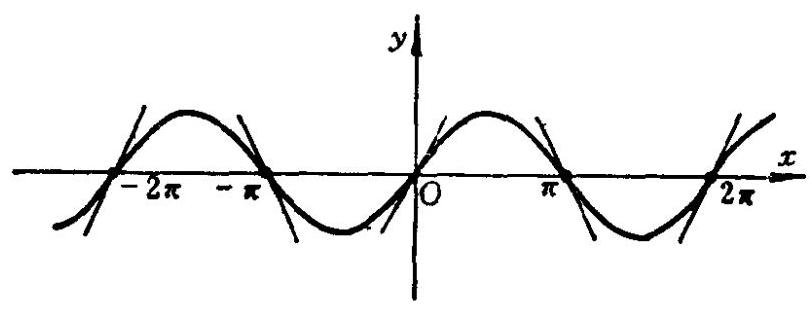
\includegraphics[max width=0.7\textwidth]{images/bo_d25ksc77aajc738obdgg_326_359_1322_811_309_0.jpg}
\end{center}
\hspace*{3em} 

图 6-16

\section*{3。函数不定型极限的计算}

导数的一个重要应用就是可用计算导数的方法求很大一类函数不定型极限,即下面的 $\mathrm{{L}^{\prime }{Hospital}}$ 法则.

定理 $6 \cdot  4 \cdot  6\left( {{\mathrm{\;L}}^{\prime }\text{ Hospital法则) 设] }a,b\lbrack }\right.$ 是任一开区间 $\left( {-\infty  \leq  a < b \leq   + \infty }\right) ,f,\mathrm{\;g} : \rbrack a,b\lbrack  \rightarrow  \mathbf{R}$ 是任意两个函数,满足下述条件:

1) $f,g$ 在 $\rbrack a,b\left\lbrack  {\text{ 上可导, }{g}^{\prime }\left( x\right)  \neq  0,\forall x \in  }\right\rbrack  a,b\lbrack$ ；

2) $\mathop{\lim }\limits_{{x \rightarrow  {a}^{ + }}}f\left( x\right)  = \mathop{\lim }\limits_{{x \rightarrow  {a}^{ + }}}g\left( x\right)  = 0$ 或 $\pm  \infty$ ;

3) $\mathop{\lim }\limits_{{r \rightarrow  {a}^{ + }}}\frac{{f}^{\prime }\left( x\right) }{{g}^{\prime }\left( x\right) } = A \in  \overline{\mathbf{R}}$ .

则我们也有
$$\mathop{\lim }\limits_{{x \rightarrow  {a}^{ + }}}\frac{f\left( x\right) }{g\left( x\right) } = A$$

当 $x \rightarrow  {b}^{ - }$ 时也有类似的结论.

证明 首先我们证明: 存在 $c \in  \rbrack a,b\lbrack$ 使得
$$g\left( x\right)  \neq  0,\;\forall x \in  \rbrack a,c\lbrack .$$

事实上,由假设 ${g}^{\prime }\left( x\right)  \neq  0,\forall x \in  \rbrack a,b\lbrack$ ,故由 Darboux 定理 (定理 $6 \cdot  3 \cdot  4$ ) 的 推 论知 ${g}^{\prime }\left( x\right)  > 0,\forall n \in  \rbrack a,b\left\lbrack  \right.$ ,或 ${g}^{\prime }\left( x\right)  < 0,\forall$  $x \in  \rbrack a,b\left\lbrack  {\text{ . 从而 }g\text{ 在 }}\right\rbrack  a,b\lbrack$ 上是严格单调的,故不论 $\mathop{\lim }\limits_{{x \rightarrow  {a}^{ + }}}g\left( x\right)  = 0$ 或 $\mathop{\lim }\limits_{{x \rightarrow  {a}^{ + }}}g\left( x\right)  =  \pm  \infty$ ,我们总可以找到一个 $c \in  \rbrack a,b\lbrack$ ,使得 $g\left( x\right)  \neq  0$ , $\forall x \in  \rbrack a,c\lbrack$ .

下面我们对 $A$ 分三种情况来讨论:

1) $A <  + \infty$ : 任取 $p,q \in  \mathbf{R}$ ,使得 $A < p < q$ .

由于 $\mathop{\lim }\limits_{{x \rightarrow  {a}^{ + }}}\frac{{f}^{\prime }\left( x\right) }{{g}^{\prime }\left( x\right) } = A$ ,故存在 ${c}_{1} \in  \rbrack a,c\lbrack$ 使得
$$\frac{{f}^{\prime }\left( x\right) }{{g}^{\prime }\left( x\right) } < p < q,\;\forall x \in  \rbrack a,{c}_{1}\lbrack .$$

于是 $\forall x,y \in  \rbrack a,{c}_{1}\lbrack$ 且 $x \neq  y$ ,由 Cauchy 中值定理有
$$\frac{f\left( x\right)  - f\left( y\right) }{g\left( x\right)  - g\left( y\right) } = \frac{{f}^{\prime }\left( \xi \right) }{{g}^{\prime }\left( \xi \right) }\;\text{ ( }\xi \text{ 介于 }x\text{ 与 }y\text{ 之间). }$$

由此得到
$$\frac{f\left( x\right)  - f\left( y\right) }{g\left( x\right)  - g\left( y\right) } < p < q,\;\forall x,y \in  \rbrack a,{c}_{1}\lbrack .$$
(*)

若 $\mathop{\lim }\limits_{{x \rightarrow  {a}^{ + }}}f\left( x\right)  = \mathop{\lim }\limits_{{x \rightarrow  {a}^{ + }}}g\left( x\right)  = 0$ ,则在 $\left( *\right)$ 中固定 $x \in  \rbrack a,{c}_{1}\lbrack$ ,并

令 $y \rightarrow  {a}^{ + }$ 得到
$$\frac{f\left( x\right) }{g\left( x\right) } < q,\;\forall x \in  \rbrack a,{c}_{1}\lbrack .$$

若 $\mathop{\lim }\limits_{{x \rightarrow  {a}^{ + }}}f\left( x\right)  = \mathop{\lim }\limits_{{x \rightarrow  {a}^{ + }}}g\left( x\right)  =  \pm  \infty$ ,则由于 $\mathop{\lim }\limits_{{x \rightarrow  {a}^{ + }}}\frac{1 - f\left( y\right) /f\left( x\right) }{1 - g\left( y\right) /g\left( x\right) }$

$= 1$ . (这里固定 $y \in  \rbrack a,{c}_{1}\left\lbrack  \right\rbrack$ . 故有 $\frac{1 - f\left( y\right) /f\left( x\right) }{1 - g\left( y\right) /g\left( x\right) } = 1 + o\left( 1\right)$  $\left( {x \rightarrow  {a}^{ + }}\right)$ . 从而由 $\left( *\right)$ 式得到
$$\frac{f\left( x\right) \left\lbrack  {1 - f\left( y\right) /f\left( x\right) }\right\rbrack  }{g\left( x\right) \left\lbrack  {1 - g\left( y\right) /g\left( x\right) }\right\rbrack  } = \frac{f\left( x\right) }{g\left( x\right) }\left\lbrack  {1 + o\left( 1\right) }\right\rbrack   < p$$

或 $\frac{f\left( x\right) }{g\left( x\right) } < \frac{p}{1 + 0\left( 1\right) }\left( {x \rightarrow  {a}^{ + }}\right)$ .

于是存在 ${c}_{2} \in  \rbrack a,{c}_{1}\left\lbrack  \right.$ 使得 $\frac{p}{1 + o\left( 1\right) } < q$ ,或
$$\frac{f\left( x\right) }{g\left( x\right) } < q,\;\forall x \in  \rbrack a,{c}_{2}\lbrack .$$

总之不论 $\mathop{\lim }\limits_{{x \rightarrow  {a}^{ + }}}f\left( x\right)  = \mathop{\lim }\limits_{{x \rightarrow  {a}^{ + }}}g\left( x\right)  = 0$ 或 $\pm  \infty$ ,我们证明了下述结论:
$$\left( {\forall q > A}\right) \left( {\exists {c}_{q} > a}\right) \left( {\forall x \in  \rbrack a,{c}_{q}\lbrack }\right)  \Rightarrow  \frac{f\left( x\right) }{g\left( x\right) } < q.\;\left( {* * }\right)$$

因此当 $A =  - \infty$ 时, $\forall M > 0$ ,若取 $q =  - M$ ,则 $\left( {* * }\right)$ 式表明
$$\mathop{\lim }\limits_{{x \rightarrow  {a}^{ + }}}\frac{f\left( x\right) }{g\left( x\right) } = A =  - \infty .$$

2) $A >  - \infty$ : 任取 $\bar{p},\bar{q} \in  \mathbf{R}$ 使得 $\bar{q} < \bar{p} < A$ .

这时我们可类似证明下述结论成立:

$\left( {\forall \bar{q} < A}\right) \left( {\exists {c}_{\bar{q}} > a}\right) \left( {\forall x \in  \rbrack a,{c}_{\bar{q}}\lbrack }\right)  \Rightarrow  \frac{f\left( x\right) }{g\left( x\right) } > \overline{{q}_{ * }}\left( {* *  * }\right)$

因此当 $A =  + \infty$ 时, $\forall M > 0$ ,若取 $\bar{q} = M$ ,则上述 $\left( {* *  * }\right)$

式表明
$$\mathop{\lim }\limits_{{x \rightarrow  a}}\frac{f\left( x\right) }{g\left( x\right) } = A =  + \infty .$$

3) $- \infty  < A <  + \infty$ ; 这时 $\forall \varepsilon  > 0$ ,若取 $q = A + \bar{\varepsilon },\bar{q} = A - \bar{\varepsilon }$ 则存在 $d = \min \left( {{c}_{q},{c}_{\bar{q}}}\right)$ 使得
$$\forall x \in  \rbrack a,d\lbrack  \Rightarrow  A - \bar{\varepsilon } < \frac{f\left( x\right) }{g\left( x\right) } < A + \bar{\varepsilon }.$$

此即表明
$$\mathop{\lim }\limits_{{x \rightarrow  a}}\frac{f\left( x\right) }{g\left( x\right) } = A$$

对 $x \rightarrow  {b}^{ - }$ 的情形可类似证明.

附注 上述 ${\mathrm{L}}^{\prime }$ Hospital法则解决了函数的 $\frac{0}{0}$ 与 $\frac{\infty }{\infty }$ 不定型的极限计算问题. $0 \cdot  \infty$ 与 $\infty  - \infty$ 不定型我们在第 4 章 $§3$ 中已经证明了通过适当处理都可以化为 $\frac{0}{0}$ 或 $\frac{\infty }{\infty }$ 不定型,至于函数的 ${1}^{\infty },{0}^{0},{\infty }^{0}$ 不定型,通过先取自然对数的方法也可以把它们化为 $0 \cdot  \infty$ 不定型. 例如设 $u{\left( x\right) }^{n + x}$ 是 ${0}^{ \circ  }$ 不定型,
$$\log u{\left( x\right) }^{v\left( x\right) } = v\left( x\right) \log u\left( x\right)$$

就是 $0 \cdot  \infty$ 不定型.

因此我们可以说, ${\mathrm{L}}^{\prime }$ Hospital法则原则上完全解决了函数的所有不定型极限的计算问题.

下面举几个例子说明 ${\mathrm{L}}^{\prime }$ Hospital法则的应用.

例 10 计算 $\mathop{\lim }\limits_{{x \rightarrow  0}}\frac{{e}^{x} - {e}^{-x}}{\sin x}$ .

这是 $\frac{0}{0}$ 不定型. 它满足 ${\mathrm{L}}^{\prime }$ Hospital法则的全部条件,并且
$$\mathop{\lim }\limits_{{x \rightarrow  0}}\frac{{\left( {e}^{x} - {e}^{-x}\right) }^{\prime }}{{\left( \sin x\right) }^{\prime }} = \mathop{\lim }\limits_{{x \rightarrow  0}}\frac{{e}^{x} + {e}^{-x}}{\cos x} = 2.$$

因此
$$\mathop{\lim }\limits_{{x \rightarrow  0}}\frac{{e}^{x} - {e}^{-x}}{\sin x} = 2.$$

例11 计算 $\mathop{\lim }\limits_{{x \rightarrow  1}}\frac{{x}^{x} - x}{\log x - x + 1}$ .

这是 $\frac{0}{0}$ 不定型. 计算这个极限时,我们必须重复应用 ${\mathrm{L}}^{\prime }\mathrm{{Ho}}$ - spital法则.
\begin{align*}
	&\mathop{\lim }\limits_{{x \rightarrow  1}}\frac{{x}^{x} - x}{\log x - x + 1} = \mathop{\lim }\limits_{{x \rightarrow  1}}\frac{{x}^{x}\left( {1 + \log x}\right)  - 1}{\frac{1}{x} - 1}\\
	&= \mathop{\lim }\limits_{{x \rightarrow  1}}\frac{{x}^{x + 1}\left( {1 + \log x}\right)  - x}{1 - x}\\
	&= \mathop{\lim }\limits_{{x \rightarrow  1}}x \cdot  \mathop{\lim }\limits_{{x \rightarrow  1}}\frac{{x}^{x}\left( {1 + \log x}\right)  - 1}{1 - x}\\
	&= \mathop{\lim }\limits_{{x \rightarrow  1}}\frac{{x}^{x}\left\lbrack  {{\left( 1 + \log x\right) }^{2} + \frac{1}{x}}\right\rbrack  }{-1}\\
	&=  - 2\text{ . }
\end{align*}

例 12 计算 $\mathop{\lim }\limits_{{x \rightarrow   + \infty }}\frac{\log x}{{x}^{a}},\mathop{\lim }\limits_{{x \rightarrow   + \infty }}\frac{{x}^{a}}{{a}^{x}}\;\left( {\alpha  > 0,a > 1}\right)$ .

它们都是 $\frac{\infty }{\infty }$ 不定型. 由 ${\mathrm{L}}^{\prime }$ Hospital法则得到
$$\mathop{\lim }\limits_{{x \rightarrow   + \infty }}\frac{\log x}{{x}^{a}} = \mathop{\lim }\limits_{{x \rightarrow   + \infty }}\frac{\frac{1}{x}}{\alpha {x}^{a - 1}} = \mathop{\lim }\limits_{{x \rightarrow   + \infty }}\frac{1}{\alpha {x}^{a}} = 0.$$

对于 $\frac{{x}^{a}}{{a}^{x}}$ ,由于 $\alpha  > 0$ 是一定数,故存在 $n \in  \mathbf{N}$ 使得 $\alpha  - n \leq  0$ . 因此对 $\frac{x}{{a}^{x}}$ 应用 $n$ 次 ${\mathrm{L}}^{\prime }$ Hospital法则得到
\begin{align*}
	&\mathop{\lim }\limits_{{x \rightarrow   + \infty }}{x}^{a} = \mathop{\lim }\limits_{{x \rightarrow   + \infty }}\frac{a{x}^{a - 1}}{{a}^{x}\log a} = \mathop{\lim }\limits_{{x \rightarrow   + \infty }}\frac{\alpha \left( {\alpha  - 1}\right) {x}^{a - 2}}{{a}^{x}{\left( \log a\right) }^{2}} = \cdots\\
	&= \mathop{\lim }\limits_{{x \rightarrow   + \infty }}\frac{a\left( {a - 1}\right) \cdots \left( {a - n + 1}\right) {x}^{a - n}}{{a}^{x}{\left( \log a\right) }^{n}}\\
	&= 0\text{ . }
\end{align*}

例 13 设 $\alpha  > 0$ ,计算 $\mathop{\lim }\limits_{{x \rightarrow  {0}^{ + }}}{x}^{\alpha }\log x$ .

这是 $0 \cdot  \infty$ 不定型. 我们把它化为 $\frac{\infty }{\infty }$ 不定型.
\begin{align*}
	&\mathop{\lim }\limits_{{x \rightarrow  {0}^{ + }}}{x}^{a}\log x = \mathop{\lim }\limits_{{x \rightarrow  {0}^{ + }}}\frac{\log x}{{x}^{-a}} = \mathop{\lim }\limits_{{x \rightarrow  {0}^{ + }}}\frac{\frac{1}{x}}{\left( {-a}\right) {x}^{-a - 1}}\\
	&= \mathop{\lim }\limits_{{x \rightarrow  0}}\frac{{x}^{a}}{-a} = 0.
\end{align*}

例 14 计算 $\mathop{\lim }\limits_{{x \rightarrow  {0}^{ + }}}{x}^{\frac{1}{1 + \log x}}$ .

这是 ${0}^{ \circ  }$ 不定型. 由 $\log {x}^{\frac{1}{1 + {\log }^{x}}} = \frac{\log x}{1 + \log x}$ 得到
$$\mathop{\lim }\limits_{{x \rightarrow  {0}^{ + }}}\log {x}^{\frac{1}{1 + \log x}} = \mathop{\lim }\limits_{{x \rightarrow  {0}^{ + }}}\frac{\log x}{1 + \log x} = \mathop{\lim }\limits_{{x \rightarrow  {0}^{ + }}}\frac{\frac{1}{x}}{\frac{1}{x}} = 1.$$

从而
\begin{align*}
	&\mathop{\lim }\limits_{{x \rightarrow  {0}^{ + }}}{x}^{\frac{1}{1 + \log x}} = \mathop{\lim }\limits_{{x \rightarrow  {0}^{ + }}}{e}^{\log {x}^{\frac{1}{1 + \log x}}}\\
	&= e\text{ . }
\end{align*}

\section*{习 题}

1. 证明下述各不等式:

1) $x < \arcsin x < \frac{x}{\sqrt{1 - {x}^{2}}}\left( {0 < x < 1}\right)$ .

2) $\log \left( {1 + x}\right)  > \frac{\operatorname{arctg}x}{1 + x}\;\left( {x > 0}\right)$ .

3) ${\int }_{a}^{b}\frac{1}{\log x}{dx} < \frac{2b}{\log b}\;\left( {{e}^{2} < a < b}\right)$ .

4) ${e}^{x} < \frac{1}{1 - x}\left( {x < 1}\right)$ .

5) ${\left( {x}^{a} + {y}^{a}\right) }^{\frac{1}{\alpha }} < {\left( {x}^{\beta } + {y}^{\beta }\right) }^{\frac{1}{\beta }}\left( {x > 0,y > 0,\beta  > a > 0}\right)$ .

2. 证明下述恒等式:
$$\forall x \in  R,{\int }_{0}^{{\sin }^{2}x}\arcsin \sqrt{t}{dt} + {\int }_{0}^{{\cos }^{2}x}\arccos \sqrt{t}{dt} = \frac{\pi }{4}.$$

3. 设函数 $f : \left\lbrack  {a,b}\right\rbrack   \rightarrow  R$ 在点 $c \in  \rbrack a,b\lbrack$ 的邻域 $B\left( {c,\delta }\right)$ 上可导,并且 ${f}^{\prime }$ 在 $c$ 处连续, ${f}^{\prime }\left( c\right)  \neq  0$ . 证明:存在 $0 < \eta  \leq  \delta$ ,使得 $f$ 在 $B\left( {c,\eta }\right)$ 上是单调的。 若 ${f}^{\prime }$ 在 $c$ 处不连续,则上述结论可以不成立. 试研究函数
$$x \mapsto  f\left( x\right)  = \left\{  \begin{array}{ll} \frac{x}{2} + {x}^{2}\sin \frac{1}{x}, & x < 0; \\  0, & x = 0. \end{array}\right.$$

1) 证明: 函数
$$x \mapsto  g\left( x\right)  = \left\{  \begin{array}{ll} {x}^{2}\sin \frac{1}{x}, & x \geq  0; \\  0, & x = 0 \end{array}\right.$$

在 $x = 0$ 的任意邻域内既有 ${g}^{\prime }\left( x\right)  = 1$ 的 $x$ 又有 ${g}^{\prime }\left( x\right)  =  - 1$ 的 $x$ .

2) 证明: 在 $x = 0$ 的任意邻域内既有 ${f}^{\prime }\left( x\right)  > 0$ 的 $x$ 又有 ${f}^{\prime }\left( x\right)  < 0$ 的 $x$ .

3) 由此推出 $f$ 在 $x = 0$ 的任意邻域内都不是单调的.

4. 设 $\left\lbrack  {a,b}\right\rbrack   = R,f : \left\lbrack  {a,b}\right\rbrack   \rightarrow  R$ 是任一函数,满足下述条件:

1) $f$ 在 $\left\lbrack  {a,b}\right\rbrack$ 上连续;

2) $\forall x \in  \rbrack a,b\left\lbrack  \right. ,{f}^{\prime }\left( {x}^{ * }\right)$ 与 $f\left( {x}^{ * }\right)$ 中至少有一个存在,并且非负 (可以为 $+ \infty )$ .

证明: $f$ 在 $\left\lbrack  {a,b}\right\rbrack$ 上是单调上升函数. 为此,

1) 假设存在 $\alpha ,\beta  \in  \left\lbrack  {a,b}\right\rbrack  ,\alpha  < \beta$ 使得 $f\left( \alpha \right)  > f\left( \beta \right)$ . 考虑直线 ${y}_{k}\left( x\right)  =$  $- k\left( {x - \alpha }\right)  + f\left( \alpha \right)$ ,证明存在 ${k}_{0} > 0$ 使得 ${y}_{{k}_{0}}\left( \beta \right)  > f\left( \beta \right)$ .

2) 令 $E = \left\{  {x \in  \left\lbrack  {\alpha ,\beta }\right\rbrack   \mid  f\left( x\right)  \geq  {x}_{{k}_{0}}\left( x\right) }\right\}  ,\xi  = \sup E$ . 证明: ${f}^{\prime }\left( {\xi }^{ + }\right)  <$  $0,{f}^{\prime }\left( {\xi }^{ - }\right)  < 0$ .

3) 由此推出 $f$ 在 $\left\lbrack  {a,b}\right\rbrack$ 上单调上升.

5. 设函数 ${f}_{3}\left\lbrack  {a,b}\right\rbrack   \rightarrow  R$ 在 $\left\lbrack  {a,b}\right\rbrack$ 上连续. 并且 $\forall x \in  \rbrack a,b\left\lbrack  {,{f}^{\prime }\left( {x}^{ * }\right) }\right.$ 与

${f}^{\prime }\left( {x}^{ - }\right)$ 中有一个存在,记它为 ${f}^{\prime }\left( {x}^{\varepsilon }\right) \left( {\varepsilon  =  \pm  }\right)$ 试利用第 3 题的结论证明
$$\mathop{\inf }\limits_{{x \in  \{ a;b\} }}{f}^{\prime }\left( {x}^{2}\right)  \leq  \frac{f\left( b\right)  - f\left( a\right) }{b - a} \leq  \mathop{\sup }\limits_{{x \in  \{ a;b\} }}{f}^{\prime }\left( {x}^{2}\right) .$$

6. 证明: 函数 $x \mapsto  \log \left( \frac{x}{\sin x}\right) ,0 < x < \frac{\pi }{2}$ 是凸的.

7. 证明: 函数
$$x \mapsto  \left\{  \begin{array}{ll} {\left( x - 2\right) }^{2}, & x \in  \lbrack 0, + \infty \lbrack , \\  {\left( x + 2\right) }^{2}, & x \in  \rbrack  - \infty ,0\rbrack  \end{array}\right.$$

在 $\rbrack  - \infty ,0\rbrack$ 与 $\lbrack 0, + \infty \lbrack$ 是凸的,但 $f$ 在 $R$ 上不是凸的.

8. 设函数 $f : I \rightarrow  J$ 与 $g : J \rightarrow  \mathrm{R}$ 是凸函数,并且 $g$ 是单调上升的,证明: $g \circ  f : I \rightarrow  R$ 也是凸函数.

${9}_{n}$ 设函数 $f : I \rightarrow  R$ 满足条件 ( $I$ 为一区间):
$$f\left( \frac{x + y}{2}\right)  \leq  \frac{1}{2}\left\lbrack  {f\left( x\right)  + f\left( y\right) }\right\rbrack  ,\forall x,y \in  I.$$

1) 证明: $\forall k = \frac{m}{{2}^{n}} \in  \left\lbrack  {0,1}\right\rbrack  ,f\left( {{kx} + \left( {1 - k}\right) y}\right)  \leq  {kf}\left( x\right)  + \left( {1 - k}\right) f\left( y\right)$ .

2) 证明: 若 $f$ 在 $I$ 上连续,则 $f$ 是凸的.

10. 设 $f : I \rightarrow  R$ 是任一 $I$ . 函数 ( $I$ 是一有限闭区间).

1) 证明: $\forall \alpha ,\beta  \in  \mathrm{R},\alpha  < \beta$ ,并且 $\left\lbrack  {\alpha ,\beta }\right\rbrack   \subset  \overset{ \circ  }{I},f$ 在 $\left\lbrack  {\alpha ,\beta }\right\rbrack$ 上是 Lipschitz函数.

2) 证明: $f$ 在 $I$ 上连续.

3) 举例说明凸函数 $f : I \rightarrow  R$ 在 $I$ 上不一定连续.

1]. 设 $f : I \rightarrow  R$ 是任一凸函数.

1) 证明: $\forall x \in  I,{f}^{\prime }\left( {x}^{ + }\right)$ 与 ${f}^{\prime }\left( {x}^{ - }\right)$ 存在并且 ${f}^{\prime }\left( {x}^{ - }\right)  \leq  {f}^{\prime }\left( {x}^{ + }\right)$ .

2) 证明: 函数 $x \mapsto  {f}^{\prime }\left( {x}^{ - }\right)$ 与 $x \mapsto  {f}^{\prime }\left( {x}^{ + }\right) ,x \in  \overset{ \circ  }{I}$ 是单调上升的. 并且
$$\forall a,b \in  \overset{ \circ  }{I},{f}^{\prime }\left( {a}^{ + }\right)  \leq  \frac{f\left( b\right)  - f\left( a\right) }{b - a} \leq  {f}^{\prime }\left( {b}^{ - }\right) .$$

12. 设 $I$ 是任一非空开区间, $f : I \rightarrow  R$ 是任一函数。证明: $f$ 是凸的充分必要条件是 $f$ 在 $I$ 上连续并且在 $I$ 上有单调上升的左、右导函数存在.

13. 设 $I$ 是任一开区间, $f : I \rightarrow  R$ 是任一函数.

1) 设 $a \in  I,f$ 是凸的. 证明: $f$ 的图形 $\Gamma$ 位于方程为 $y = f\left( a\right)  + m\left( {x - a}\right)$ 的直线的上方,当且仅当 ${f}^{\prime }\left( {a}^{ - }\right)  \leq  m \leq  {f}^{\prime }\left( {a}^{ + }\right)$ .

2) 设 $f$ 在 $I$ 上连续,右 (或左) 可导,且满足下述不等式:
\begin{align*}
	&\forall a,x \in  I,f\left( x\right)  \geq  f\left( a\right)  + {f}^{\prime }\left( {a}^{ + }\right) \left( {x - a}\right)\\
	&\left( {f\left( x\right)  \geq  f\left( a\right)  + {f}^{\prime }\left( {a}^{ - }\right) \left( {x - a}\right) }\right) .
\end{align*}

证明: $f$ 是凸的.

14. 设 $f : \rbrack a,b\lbrack  \rightarrow  R$ 是 ${C}^{1}$ 类的,并且是严格凸的 (即 $\forall {x}_{1},{x}_{2} \in  \rbrack a,b\lbrack$ , $\forall {\alpha }_{1},{\alpha }_{2} \in  \left\lbrack  {0,1}\right\rbrack$ 且 ${\alpha }_{1} + {\alpha }_{2} = 1$ 满足:
$$\left. {f\left( {{\alpha }_{1}{x}_{1} + {\alpha }_{2}{x}_{2}}\right)  < {\alpha }_{1}f\left( {x}_{1}\right)  + {\alpha }_{2}f\left( {x}_{2}\right) }\right) .$$

1) 证明: $f$ 的图形 $\Gamma$ 上的每一点的切线的斜率所组成的实数集合是一开区间 $J$ 。 2) 证明: ${f}^{\prime } : \rbrack a,b\lbrack  \rightarrow  J$ 是可逆的. 记 $k : J \rightarrow  \rbrack a,b\lbrack$ 为 ${f}^{\prime }$ 的反函数.

3) $\forall \lambda  \in  J$ ,定义函数 $\left. {{h}_{\lambda } : }\right\rbrack  a,b\lbrack  \rightarrow  R$ 如下:
$${h}_{\lambda }\left( x\right)  = {\lambda x} - f\left( x\right) ,\forall x \in  \rbrack a,b\lbrack .$$

证明: ${h}_{\lambda }$ 在 $\rbrack a,b\lbrack$ 上有唯一的极大值点,记它为 ${x}_{\lambda }$ .

4) 定义函数 $g : J \rightarrow  R$ 如下:
$$g\left( \lambda \right)  = {h}_{\lambda }\left( {x}_{\lambda }\right)  = \mathop{\sup }\limits_{{x \in  {D}_{\lambda }}}\left( {{\lambda x} - f\left( x\right) }\right) ,\forall \lambda  \in  J.$$

试找出函数 $f,k,g$ 所满足的关系式.

5) 证明: $g$ 在 $J$ 上连续.

6) 证明: $g$ 在 $J$ 上是凸函数.

15. 设函数 $f : \left\lbrack  {a\text{ 、 }b}\right\rbrack   \rightarrow  R$ 在 $\left\lbrack  {a\text{ 、 }b}\right\rbrack$ 上 2 次可导,证明: $\forall x \in  \rbrack a,b\lbrack$ ,
$${f}^{\prime \prime }\left( x\right)  = \mathop{\lim }\limits_{{h \rightarrow  0}}\frac{f\left( {x + h}\right)  + f\left( {x - h}\right)  - {2f}\left( x\right) }{{h}^{2}}.$$

16. 计算下列各极限值:

1) $\mathop{\lim }\limits_{{x \rightarrow  0}}\frac{x - \operatorname{tg}x}{{x}^{3}}$ ,

2) $\mathop{\lim }\limits_{{x \rightarrow  0}}\frac{x{e}^{x} - \log \left( {1 + x}\right) }{{x}^{2}}$ ,

3) $\mathop{\lim }\limits_{{x \rightarrow  0}}\sin x\log x$ ,

4) $\mathop{\lim }\limits_{{x \rightarrow  1}}\left( {\frac{1}{\log x} - \frac{1}{x - 1}}\right)$ ,

5) $\mathop{\lim }\limits_{{x \rightarrow  0}}\left\lbrack  {\frac{1}{\log \left( {x + \sqrt{1 + {x}^{2}}}\right) } - \frac{1}{\log \left( {1 + x}\right) }}\right\rbrack$ ,

6) $\mathop{\lim }\limits_{{x \rightarrow  {1}^{ - }}}{\left( 1 - {x}^{2}\right) }^{\frac{1}{\log \left( {1 - x}\right) }}$ ,

7) $\mathop{\lim }\limits_{{x \rightarrow  0}}{\left( \frac{\operatorname{tg}x}{x}\right) }^{\frac{1}{{x}^{2}}}$ ,

8) $\mathop{\lim }\limits_{{x \rightarrow  0}}{\left( \frac{\cos x}{\operatorname{ch}x}\right) }^{\frac{1}{2}}$ ,

9) $\lim {\left( \operatorname{ctg}x\right) }^{\ln x}$ 10) $\lim {\left( \sin x\right) }^{1 + x}$ .
$$\text{ 乙方法 }$$

$x \rightarrow  \frac{\pi }{3}$ For every

